% !Mode:: "TeX:UTF-8"
% !TEX program  = xelatex

\documentclass[bwprint]{gmcmthesis}
% \documentclass[bwprint,fontset=fandol]{gmcmthesis} % Overleaf 等在线平台需要用这一行。
\usepackage[framemethod=TikZ]{mdframed}
\usepackage{amssymb}
\usepackage{bm}
\usepackage{dsfont}
\newcommand{\E}{\mathbb{E}}

\usepackage{subfig}
\usepackage{colortbl}
\usepackage{threeparttable}
\usepackage{booktabs}
\usepackage{xltabular}

\newcommand{\clip}[1]{\operatorname{clip}\left(#1\right)}
\definecolor{color2}{rgb}{0.36,0.62,0.84}
% \definecolor{color3}{rgb}{0.8235,0.8706,0.9373}
\definecolor{color3}{rgb}{0.88,0.92,0.96}
\definecolor{color4}{rgb}{0.96,0.97,0.98}   % {0.9176,0.9373,0.9686}

% 算法
\usepackage[noend]{algpseudocode}
\usepackage{algorithmicx,algorithm}
\floatname{algorithm}{算法}
\renewcommand{\algorithmicrequire}{\textbf{输入:}}
\renewcommand{\algorithmicensure}{\textbf{输出:}}
\numberwithin{equation}{section}
\numberwithin{figure}{section}
\numberwithin{table}{section}
\newcommand{\red}[1]{\textcolor{red}{#1}}
\newcommand{\blue}[1]{\textcolor{blue}{#1}}


\title{算力约束下提升大语言模型能力的资源配置建模}   % 标题
\baominghao{26102860508}   % 参赛队号
\schoolname{东南大学}   % 学校名称(跨校加角标$^1$标注对应关系)
\membera{杨嘉诚}   % 队员A(跨校加角标$^1$标注对应关系)
\memberb{李邵恺}   % 队员B(跨校加角标$^1$标注对应关系)
\memberc{许圣炜}   % 队员C(跨校加角标$^1$标注对应关系)
\begin{document}

% 生成标题
\maketitle


\begin{abstract}    % 摘要
    大语言模型的训练依赖大规模算力 $C$，其能力提升受参数量 $N$、训练数据量 $D$、数据质量 $Q$ 及领域配比 $\textit{\textbf{p}}$ 等因素共同影响。在算力增长放缓的背景下，如何协调各类资源投入并提高训练效率，已成为亟需解决的重要问题。本文分别从质量与配比评价、广义标度律模型、算力约束资源优化及综合能力演进方面，研究有限算力条件下的资源配置和能力提升策略。
    
    针对问题一：质量指标的含义与方向存在差异，部分指标相互冲突，领域配比还受到总份额约束。本文采用受限 \textbf{CRITIC 赋权}与 \textbf{Huber 鲁棒估计}，对 22 项质量指标进行综合评价，通过分歧度与稳健极差识别冲突，并利用 \textbf{ILR 变换}和\textbf{二次多输出岭回归}建立 $\textit{\textbf{p}}$—Loss 关系。结果表明，抽样集与扩展集的平均质量评价基本一致，指标冲突主要涉及文本长度、重复特征和数字比例；配比模型在同规模检验中的\textbf{决定系数}约为 0.86。
    
    针对问题二：规模、质量与配比数据来自不同实验体系，需要统一其作用关系并避免重复计入质量贡献。本文在经典双幂律中引入\textbf{配比相对响应}与\textbf{额外质量修正}，采用分阶段稳健估计建立\textbf{广义标度律}，并推导各因素的边际收益、弹性及质量与参数规模的等效替代条件。结果表明，加入质量项后，半合成质量数据的分组验证 \textbf{RMSE} 降低约 58\%；在选定参考情景下，质量提高 0.1 所带来的预测改善，约等效于参数规模增加三分之一。
    
    针对问题三：基础训练、质量提升和长上下文计算共同占用有限预算，不同成本机制会改变资源分配策略。本文以广义标度律预测 Loss 最小为目标，建立统一算力约束下的优化模型，通过解析消去数据量 D 实现\textbf{降维}，\textbf{$(\log_{10}N, Q)$ 网格}上搜索，\textbf{SLSQP 算法}在同一可行域内细化求解，并比较三类质量成本机制与不同上下文情景。结果表明，低预算下的质量投入对成本形式较为敏感；由题设成本代理式得到，上下文长度约为 3 万 tokens 时，注意力开销与基础训练开销相当；在选定的固定预算情景下，经验候选配方较参考配方的预测损失降低约 2\%。
    
    针对问题四：训练损失与任务能力的评价口径不同，历史能力变化还受到规模以外因素的共同影响。本文建立单调的 Loss—Benchmark 映射，结合\textbf{模型族}与\textbf{类型控制}、非规模\textbf{时间动力学模型}和 \textbf{Shapley 分解}，分析能力变化的条件贡献，并利用算力情景与\textbf{分层 Bootstrap} 预测能力前沿及其不确定性。在指数型质量成本、固定上下文且非规模趋势保留一半的示例情景下，算力年增 10\% 时，聊天／微调模型在附件截止日后一年和两年的前沿得分分别约为 44 分和 47 分。

    \keywords{Huber鲁棒估计；ILR变换；广义标度律；SLSQP算法；分层Bootstrap}    % 关键字
\end{abstract}

\pagestyle{plain}

\tableofcontents    % 目录
\clearpage


\section{问题重述}  % 1
近年来，大语言模型在自然语言理解、知识推理、代码生成和复杂任务规划等方面取得了快速进展。模型能力的提升通常与参数规模、训练数据量和训练算力的增长密切相关。除参数量和数据量外，训练数据的质量与领域配比同样会影响模型性能。QuRating 表明，可以从多个质量侧面对预训练文本进行评价和筛选\textsuperscript{\cite{wettig2024qurating}}。网页、书籍、代码、论文和问答社区等数据源在教育价值、流畅度、专业性、重复程度和噪声水平上存在明显差异，不同质量指标还可能对同一文本给出相互冲突的判断。而训练语料的领域份额之和为 1，提高某一领域占比必然压缩其他领域的份额。RegMix 和数据混合规律研究进一步说明，可以利用性能代理模型预测不同训练配方的表现，并据此讨论数据混合方案\textsuperscript{\cite{liu2025regmix,ye2025mixing}}。

同时，提高数据质量需要额外的清洗、筛选和生成成本，扩大上下文长度也会增加注意力计算开销。在给定总算力预算下，对某一资源增加投入意味着压缩其他资源的可用预算。由此，需要比较不同质量成本机制和上下文长度下的最优参数量、数据量与质量水平，并分析预算增长过程中资源投入结构的阶段性变化。还注意到，真实大语言模型的能力演化不仅来自规模扩张，还可能受到网络架构、优化算法等非规模因素影响。观察型标度律研究表明，在公共模型数据中分析能力变化时，需要考虑模型族、规模指标和观测口径之间的差异\textsuperscript{\cite{ruan2024observational}}。

基于上述背景，本题围绕数据价值评估、广义标度律、算力约束下的资源优化以及模型能力演化展开递进研究，为有限算力条件下提升大语言模型能力提供可解释、可验证的量化依据。

\textbf{问题一：}
附件 A1--A3 中质量信号数据的每条文本包含 22 个质量指标，要求使用 A1 抽样集以及 A2、A3 扩展集的全部记录，建立样本级和领域级质量评分 $Q$，并检验扩展集与抽样集是否具有一致结论。当不同指标对同一文本给出显著不一致的判断时，还需定义冲突、分析来源并提出消解方法。A4--A15 的 RegMix 配方实验数据。每个配方由 17 个 The Pile 子领域的份额构成，份额非负且和为 1；对应结果为 13 个验证领域的交叉熵 Loss。需要利用 A4/A5 建模，在 A6--A11 的 1M、60M、1B 检验集上验证，并利用 A12--A15 讨论 10B 和 70B 外推结论的稳健性。若将 $Q$ 引入配比模型，必须说明映射和不确定性。

\textbf{问题二：}
在问题一得到的质量评分与领域配比模型基础上，建立能够同时描述 $N$、$D$、$Q$ 与 $\bm p$ 影响的广义标度律，并结合 附件 B1，B6（或B7，B8） 计算广义标度律的相关参数。模型在特定条件下能够退化为经典标度律，同时进一步求解参数量、数据量和质量的边际收益，给出质量提高与参数扩容达到同等性能时的替代条件，并分析领域配比的局部互补或替代关系。其他附件 B 中的数据用做广义标度律的验证和外推。

\textbf{问题三：}
在问题二广义标度律的基础上，把参数量、训练数据量、数据质量、领域配比和上下文长度纳入统一的算力预算，C7 定义了上下文长度的取值。要求针对不同总算力与三类质量提升成本函数，求解使预测 Loss 最小的资源配置，并分析新增预算如何在基础训练、质量提升和长上下文注意力之间转移。由于领域配比的跨规模迁移证据有限，需要额外考虑经验候选配比的敏感性结果。

\textbf{问题四：}
通过附件 C5 或 C6，计算 Loss--Benchmark 桥接关系，并建立模型综合能力。同时结合附件 C1--C4，刻画大语言模型能力随时间的演化。在控制参考规模效应后，将历史改善分解为规模项与非规模时间项，并在算力增长放缓的外生情景下调用问题三求解器，预测未来 12 个月和 24 个月的条件能力前沿，同时报告桥接误差、时间留出误差、Bootstrap 区间及外推边界。

\begin{figure}[H]
    \centering
    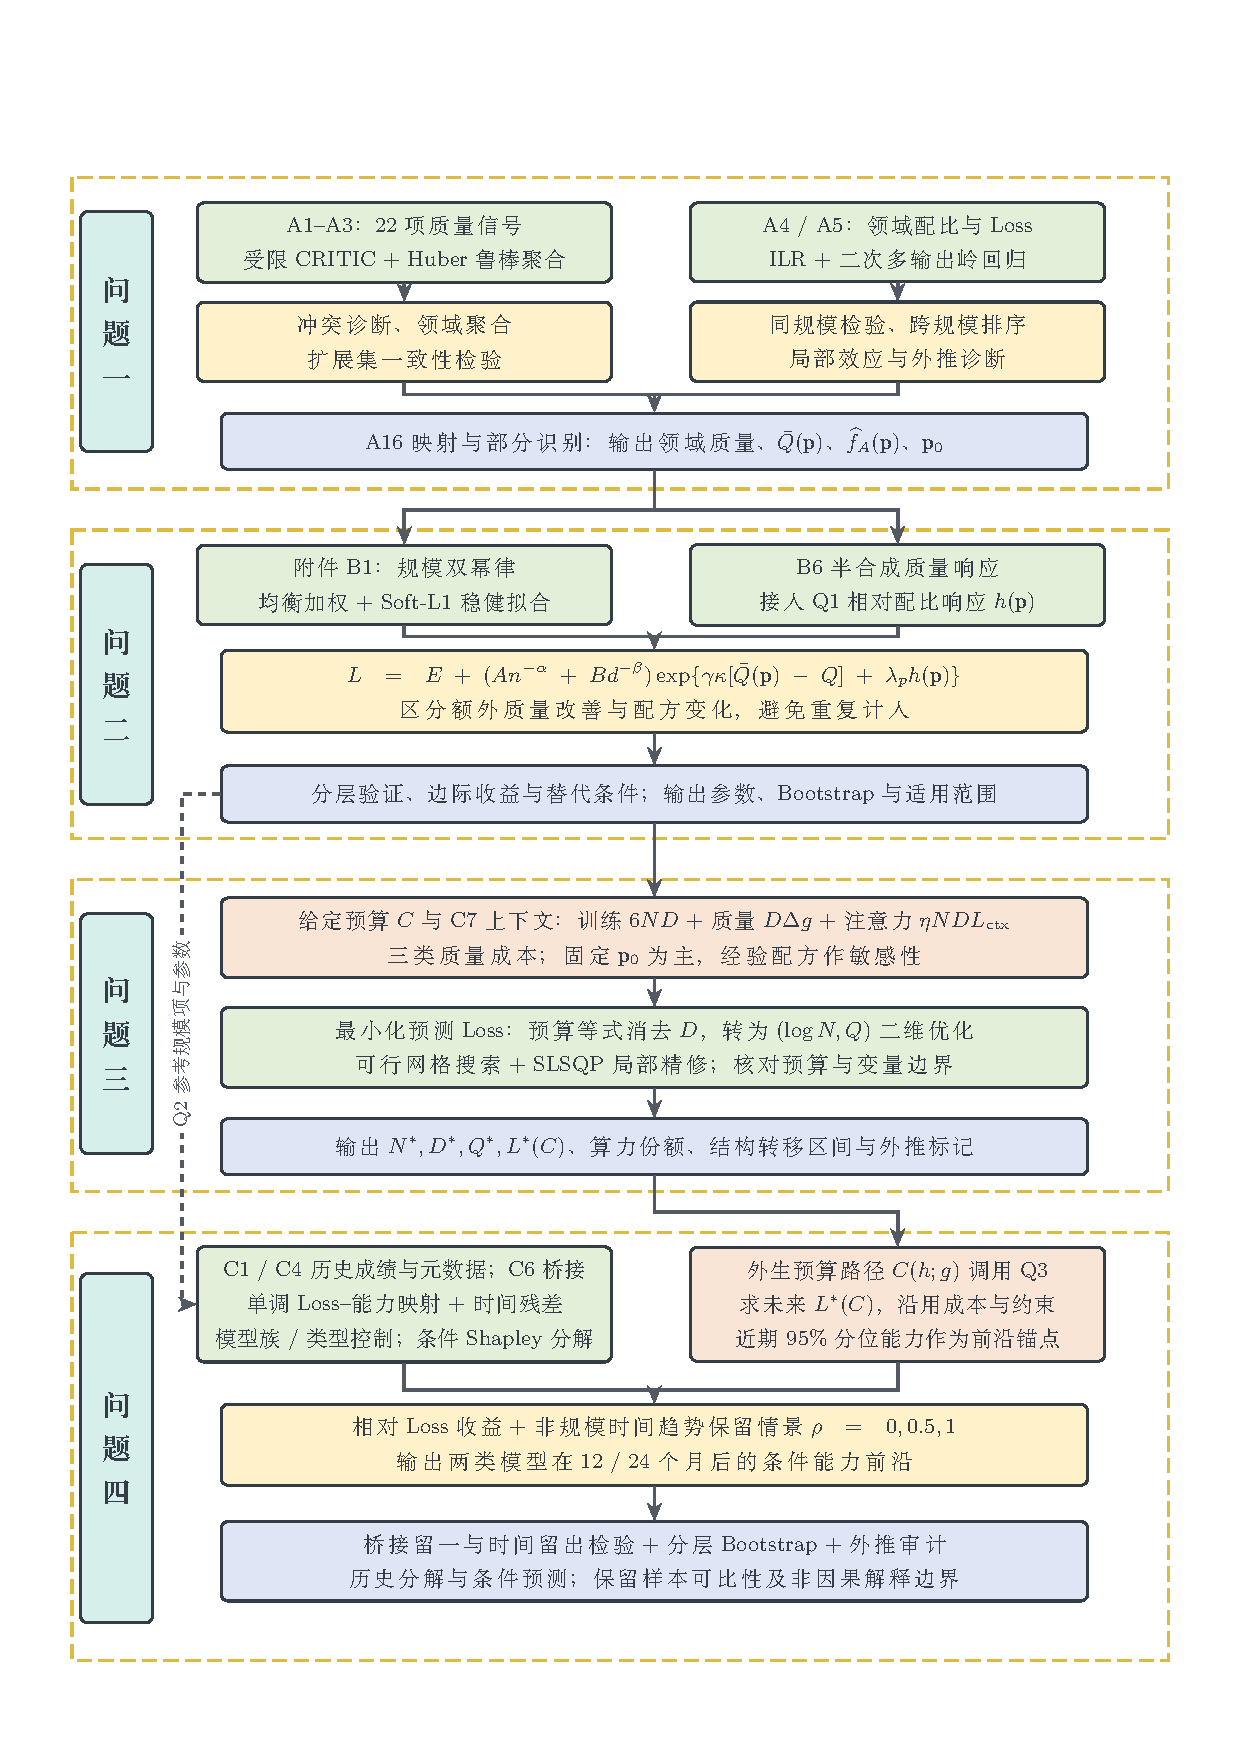
\includegraphics[width=0.81\textwidth]{figures/flowchart.pdf}
    \caption{技术路线图}
    \label{fig:qualitydomain}
\end{figure}

\section{模型假设}  % 2
\begin{enumerate}[label=\textbf{H\arabic*.},leftmargin=2.5em]
    \item 不同来源质量改善与领域配比的相对效应具有有限可迁移性。
    \item 参考条件下广义标度律退化为经典双幂律。
    \item 可比评测条件下，训练损失与任务能力具有单调关联。
    \item 能力演化规律在给定情景下具有短期延续性。
    
\end{enumerate}


% \section{定义与符号说明}   % 3
% \begin{table}[H]    % table 3.1
%     \centering
%     \caption{主要符号}
%     \label{tab:symbols}
%     \begin{tabularx}{0.92\textwidth}{cX}
%         \toprule
%         符号 & 含义 \\
%         \midrule
%         $i,j,d,k,r,s$ & 文本、质量指标、质量领域、配方领域、Loss 验证域、模型规模的下标 \\
%         $x_{ij}$ & 列表压缩后的原始质量指标 \\
%         $S_{ij}$ & 方向统一后的质量得分，取值在 $[0,1]$ \\
%         $w_j$ & 第 $j$ 个质量指标的受限 CRITIC 权重 \\
%         $Q_i,Q_d$ & 文本级综合质量与领域级质量 \\
%         $D_i,R_i$ & 文本的加权分歧度与 90\%--10\% 稳健极差 \\
%         $Conf_i$ & 文本质量评分置信度 \\
%         $\bm p_i$ & 17 维领域配比，满足非负且和为 1 \\
%         $\bm z_i$ & 配比的 16 维 ILR 坐标 \\
%         $L_{ir},\widehat L_{ir}$ & 观测和预测的第 $r$ 个验证域 Loss \\
%         $ME_k,INT_{jk}$ & 领域边际效应和两领域二阶组合效应 \\

%         $N,D$ & 模型参数个数与训练 token 数 \\
%         $n,d$ & 归一化规模，$n=N/10^9$、$d=D/10^{11}$ \\
%         $Q,\bar Q(\bm p)$ & 当前语料质量与配方的常规质量基准 \\
%         $\bm p_0,Q_0$ & 参考配比与参考质量，$Q_0=\bar Q(\bm p_0)$ \\
%         $f_A(\bm p),h(\bm p)$ & 问题一对13个验证领域的平均预测 Loss 及其对数相对响应 \\
%         $E,A,B,\alpha,\beta$ & 渐近 Loss、规模项幅度及衰减指数 \\
%         $\gamma,\kappa$ & 质量响应系数与质量量尺换算系数 \\
%         $\lambda_p$ & 配比迁移强度，与问题一岭惩罚 $\lambda$ 区分 \\
%         $G(Q,\bm p)$ & 质量和配比的乘性修正因子 \\
%         $X,Y$ & 参数受限项 $An^{-\alpha}$ 与数据受限项 $Bd^{-\beta}$ \\
%         $\omega_i$ & 问题二拟合记录的均衡权重 \\
%         $U_n,U_d,U_Q$ & 单位规模、数据量及质量的边际降损收益 \\
%         $c_n,c_Q$ & 单位归一化参数量及质量的边际成本 \\
%         $N_{\mathrm{eq}},\Delta Q$ & 等效参数量与质量的绝对提高量 \\
%         $I_{jk},\varepsilon_p$ & 参考点领域混合导数与份额差分步长 \\
%         $C,C_{train},C_{qual},C_{attn}$ & 总算力预算及基础训练、质量提升、注意力开销 \\
%         $g_c(Q),L_{ctx},\eta$ & 质量成本函数、上下文长度与注意力成本系数 \\
%         $Q_b,Q^*$ & 当前配比的基线质量与优化后的质量 \\
%         $S_i,z(S_i)$ & 六任务综合能力分数及其截断 logit 变换 \\
%         $H(L),G(L)$ & Loss 到综合能力分数及其 logit 的桥接函数 \\
%         $r_i,\tau$ & 扣除参考规模项后的残差与年时间趋势 \\
%         $\Delta_{scale},\Delta_{time}$ & 条件 Shapley 规模贡献与非规模时间贡献 \\
        
%         \bottomrule
%     \end{tabularx}
% \end{table}

\section{定义与符号说明}   % 3
% 去掉原来的 \begin{table}[H] ... \end{table}，xltabular本身不是浮动体
\begin{xltabular}{0.92\textwidth}{cX}
    \caption{主要符号}
    \label{tab:symbols}\\
    \toprule
    符号 & 含义 \\
    \midrule
    \endfirsthead  % 第一页表头结束

    % ===== 后续页面重复表头（续表）=====
    \multicolumn{2}{l}{\textit{续表\ref{tab:symbols}}}\\
    \toprule
    符号 & 含义 \\
    \midrule
    \endhead

    % 每一页底部（非最后一页）显示“接下页”
    \midrule
    \multicolumn{2}{r}{\small 接下页}
    \endfoot

    % 最后一页底部
    \bottomrule
    \endlastfoot

    $i,j,d,k,r,s$ & 文本、质量指标、质量领域、配方领域、Loss 验证域、模型规模的下标 \\
    $x_{ij}$ & 列表压缩后的原始质量指标 \\
    $S_{ij}$ & 方向统一后的质量得分，取值在 $[0,1]$ \\
    $w_j$ & 第 $j$ 个质量指标的受限 CRITIC 权重 \\
    $Q_i,Q_d$ & 文本级综合质量与领域级质量 \\
    $D_i,R_i$ & 文本的加权分歧度与 90\%--10\% 稳健极差 \\
    $Conf_i$ & 文本质量评分置信度 \\
    $\bm p_i$ & 17 维领域配比，满足非负且和为 1 \\
    $\bm z_i$ & 配比的 16 维 ILR 坐标 \\
    $L_{ir},\widehat L_{ir}$ & 观测和预测的第 $r$ 个验证域 Loss \\
    $ME_k,INT_{jk}$ & 领域边际效应和两领域二阶组合效应 \\
    $N,D$ & 模型参数个数与训练 token 数 \\
    $n,d$ & 归一化规模，$n=N/10^9$、$d=D/10^{11}$ \\
    $Q,\bar Q(\bm p)$ & 当前语料质量与配方的常规质量基准 \\
    $\bm p_0,Q_0$ & 参考配比与参考质量，$Q_0=\bar Q(\bm p_0)$ \\
    $f_A(\bm p),h(\bm p)$ & 问题一对13个验证领域的平均预测 Loss 及其对数相对响应 \\
    $E,A,B,\alpha,\beta$ & 渐近 Loss、规模项幅度及衰减指数 \\
    $\gamma,\kappa$ & 质量响应系数与质量量尺换算系数 \\
    $\lambda_p$ & 配比迁移强度，与问题一岭惩罚 $\lambda$ 区分 \\
    $G(Q,\bm p)$ & 质量和配比的乘性修正因子 \\
    $X,Y$ & 参数受限项 $An^{-\alpha}$ 与数据受限项 $Bd^{-\beta}$ \\
    $\omega_i$ & 问题二拟合记录的均衡权重 \\
    $U_n,U_d,U_Q$ & 单位规模、数据量及质量的边际降损收益 \\
    $c_n,c_Q$ & 单位归一化参数量及质量的边际成本 \\
    $N_{\mathrm{eq}},\Delta Q$ & 等效参数量与质量的绝对提高量 \\
    $I_{jk},\varepsilon_p$ & 参考点领域混合导数与份额差分步长 \\
    $C,C_{train},C_{qual},C_{attn}$ & 总算力预算及基础训练、质量提升、注意力开销 \\
    $g_c(Q),L_{ctx},\eta$ & 质量成本函数、上下文长度与注意力成本系数 \\
    $Q_b,Q^*$ & 当前配比的基线质量与优化后的质量 \\
    $S_i,z(S_i)$ & 六任务综合能力分数及其截断 logit 变换 \\
    $H(L),G(L)$ & Loss 到综合能力分数及其 logit 的桥接函数 \\
    $r_i,\tau$ & 扣除参考规模项后的残差与年时间趋势 \\
    $\Delta_{scale},\Delta_{time}$ & 条件 Shapley 规模贡献与非规模时间贡献 \\
\end{xltabular}



\section{问题一}   % 4
    \subsection{问题分析}   % 4.1
    质量信号的主要困难不是简单加权，而是输出结构和语义不同。二分类模型输出 logits，有序分类器输出 6 维 logits，Qurater 给出多个并列质量侧面\textsuperscript{\cite{wettig2024qurating}}，而 RedPajama 统计量为连续标量。若直接对列表取均值，会混淆概率、等级和不同侧面的含义。其次，``词数越多越好''或``数字比例越低越好''并不适用于所有领域，必须将这类指标视为目标型而非强行设定单调方向。最后，扩展集中 arxiv 和 github 的记录数远大于其他领域，若直接用全体数据估计权重，会让领域规模影响指标权重。因此本文只用覆盖 7 个领域的 A1 估计归一化参数和权重，再把同一变换应用到 A2/A3。

    质量指标的分歧可能来自真实的多面性，也可能来自分类器误差、文本格式或极端长度。仅用最大值减最小值会被单项异常放大，仅用方差又可能把多个指标的系统性对立平均掉。本文联合使用加权分歧度和 90\%--10\% 稳健极差，并以 A1 分歧度的高分位数确定阈值。综合评分借鉴 Huber 鲁棒估计\textsuperscript{\cite{huber1964robust}}，使冲突记录中的离群指标自动降权，而不是删除整条文本。

    17 个领域份额属于成分数据。在含截距的回归中同时纳入全部原始份额会产生完全共线性，成分数据分析强调以分量间的相对比例刻画其变化\textsuperscript{\cite{aitchison1982compositional}}。同时，13 个验证域的 Loss 相关但不完全相同，需要多输出建模。RegMix 将数据配比优化转化为性能回归预测，并检验小模型配方排序向较大模型迁移的效果\textsuperscript{\cite{liu2025regmix}}。本题 RegMix 的训练表只有 512 个配方，若使用高复杂度黑箱模型，不利于效应解释且容易过拟合。本文采用 ILR 坐标上的二次岭回归：ILR 将配比映射到正交的对数比坐标\textsuperscript{\cite{egozcue2003ilr}}，二次项表达组合关系，岭惩罚用于降低共线性带来的估计不稳定性\textsuperscript{\cite{hoerl1970ridge}}。

    % \begin{figure}[H]
    %   \centering
    %   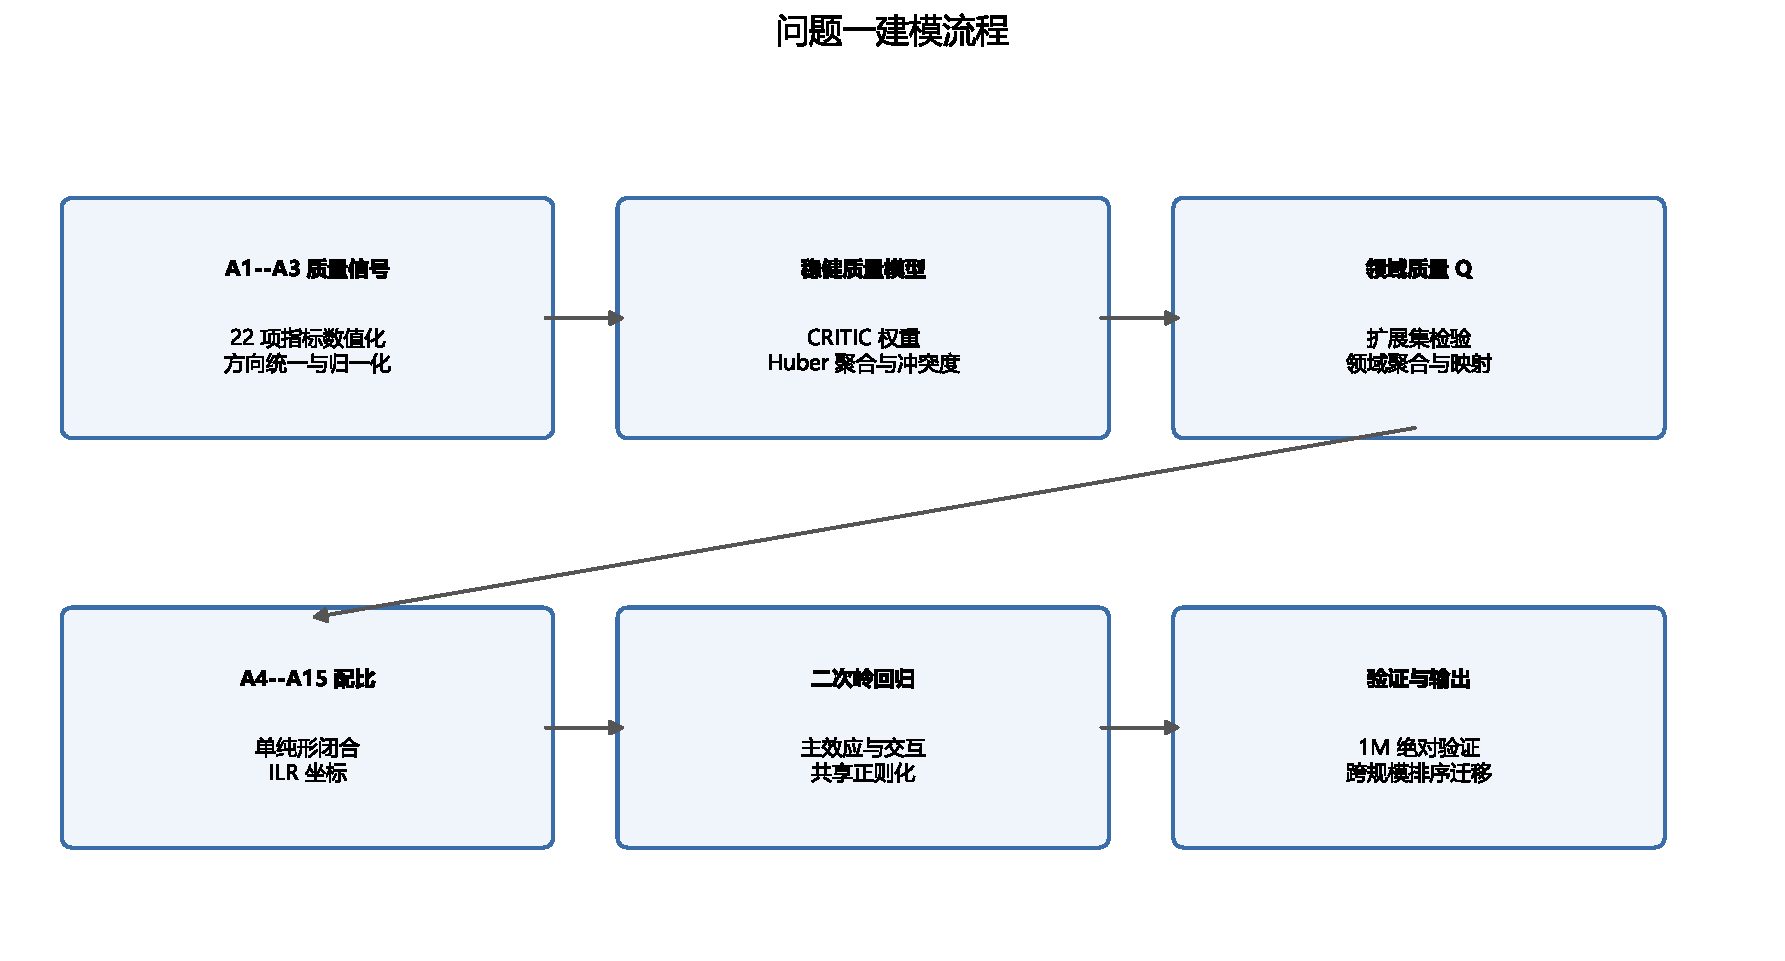
\includegraphics[width=0.96\textwidth]{figures/q1_fig01_modeling_workflow.pdf}
    %   \caption{问题一建模流程 (待更新)}
    %   \label{fig:workflow}
    % \end{figure}
    
    \subsection{模型建立}   % 4.2
        \subsubsection{列表型质量信号标量化}  % 4.2.1 
        设文本 $i$ 的指标 $j$ 原始输出为 $x_{ij}$。标量字段直接保留；8 个列表型字段按输出含义处理。

        对 `fluency\_en' 和 `ad\_en' 的二分类 logits $(a_0,a_1)$，取正类概率：
        \begin{equation}
        x_{ij}=\frac{\exp(a_1)}{\exp(a_0)+\exp(a_1)}.
        \label{eq:binary}
        \end{equation}
        
        对四个 `modernbert\_*' 的 6 级有序 logits，取归一化期望等级：
        \begin{equation}
        x_{ij}=\sum_{c=0}^{5}\frac{c}{5}
        \frac{\exp(a_c)}{\sum_{h=0}^{5}\exp(a_h)}.
        \label{eq:ordinal}
        \end{equation}
        
        `qurater' 的四个分量对应 QuRating 的并列质量侧面\textsuperscript{\cite{wettig2024qurating}}。本文在此基础上进行标量化，分别经逻辑函数后求平均：
        \begin{equation}
        x_{ij}=\frac{1}{4}\sum_{c=1}^{4}\frac{1}{1+\exp(-a_c)}.
        \label{eq:qurater}
        \end{equation}
        
        `fineweb\_edu' 的列表仅含一个元素，直接取其值。这样避免了对 logits 直接平均造成的量纲错误。


        \subsubsection{方向统一与缺失处理}   % 4.2.2 
        以 A1 为参考样本，计算指标 $j$ 的 1\%、50\%、99\% 分位数 $q_{.01,j},q_{.50,j},q_{.99,j}$，并将极端值缩尾到该区间。效益型指标转换为
        \begin{equation}
        S_{ij}=\frac{\clip(x_{ij})-q_{.01,j}}{q_{.99,j}-q_{.01,j}},
        \label{eq:benefit}
        \end{equation}
        成本型指标转换为
        \begin{equation}
        S_{ij}=1-\frac{\clip(x_{ij})-q_{.01,j}}{q_{.99,j}-q_{.01,j}}.
        \label{eq:cost}
        \end{equation}
        
        词数、句数、数字比例和平均词长设为目标型指标：
        \begin{equation}
        S_{ij}=\begin{cases}
        1-\dfrac{q_{.50,j}-x_{ij}}{q_{.50,j}-q_{.01,j}},&x_{ij}\le q_{.50,j},\\[6pt]
        1-\dfrac{x_{ij}-q_{.50,j}}{q_{.99,j}-q_{.50,j}},&x_{ij}>q_{.50,j}.
        \end{cases}
        \label{eq:target}
        \end{equation}
        所有结果截断到 $[0,1]$，从而统一为越高越好。缺失值先用同领域中位数填补，再用 A1 全局中位数兜底；另保留原始覆盖率，防止填补后的记录被误认为信息完整。
        
        
        \subsubsection{受限 CRITIC 权重}    % 4.2.3
        在方向统一后的 A1 得分上计算标准差 $\sigma_j$ 和相关系数 $\rho_{jh}$。经典 CRITIC 方法综合指标的变异性与冲突性确定客观权重\textsuperscript{\cite{diakoulaki1995critic}}。本文借鉴其赋权思想，将相关系数替换为绝对相关系数，以衡量正负相关所体现的信息冗余，定义改进信息量与权重为
        \begin{equation}
        C_j=\sigma_j\sum_{h=1}^{22}(1-|\rho_{jh}|),\qquad
        w_j^{(c)}=\frac{C_j}{\sum_hC_h}.
        \label{eq:critic}
        \end{equation}
        
        为避免噪声造成权重过度集中，将 CRITIC 权重与等权重各占一半，并限制单项范围：
        \begin{equation}
        \widetilde w_j=\frac12\frac1{22}+\frac12w_j^{(c)},\qquad
        w_j=\frac{\clip(\widetilde w_j,0.5/22,2/22)}
        {\sum_h\clip(\widetilde w_h,0.5/22,2/22)}.
        \label{eq:weight}
        \end{equation}
        
        全量运行中，数字字符比例、专业性、句数、词数和流畅度权重较高，分别为 0.0609、0.0548、0.0538、0.0527 和 0.0526；全部指标仍保留正权重。

        
        \subsubsection{Huber 鲁棒综合质量分}   % 4.2.4
        若直接取加权均值，单个严重偏离的指标仍可能拉动结果。本文借鉴 Huber 鲁棒位置估计\textsuperscript{\cite{huber1964robust}}，构造加权质量聚合目标：
        \begin{equation}
        Q_i=\arg\min_{q\in[0,1]}\sum_{j=1}^{22}w_j
        \rho_{1.345}\!\left(\frac{S_{ij}-q}{\widehat\sigma_i}\right),
        \label{eq:huberq}
        \end{equation}
        其中
        \begin{equation}
        \widehat\sigma_i=1.4826\operatorname{median}_{j}|S_{ij}-q|,
        \qquad
        \rho_c(u)=\begin{cases}
        \tfrac12u^2,&|u|\le c,\\
        c|u|-\tfrac12c^2,&|u|>c.
        \end{cases}
        \label{eq:huber}
        \end{equation}
        通过迭代重加权求解式式~\eqref{eq:huberq}。在指标一致时，该估计接近加权均值；出现少数异常指标时，其边际权重随残差增大而下降。

        
        \subsubsection{冲突定义、置信度与成因贡献}   % 4.2.5
        定义加权分歧度和稳健极差为
        \begin{equation}
        D_i=\sqrt{\sum_jw_j(S_{ij}-Q_i)^2},\qquad
        R_i=P_{90}(S_{i\cdot})-P_{10}(S_{i\cdot}).
        \label{eq:disagreement}
        \end{equation}
        
        以 A1 的 $D_i$ 的 95\% 分位数为 $\tau_D$，显著冲突定义为
        \begin{equation}
        I_i=\mathds{1}(D_i>\tau_D\ \land\ R_i>0.60).
        \label{eq:conflict}
        \end{equation}
        全量计算得到 $\tau_D=0.38725$。联合条件既要求总体分歧较大，也要求指标两端存在实质距离。
        
        评分置信度定义为
        \begin{equation}
        Conf_i=Coverage_i\left(1-\min\left\{\frac{D_i}{0.50},1\right\}\right).
        \label{eq:confidence}
        \end{equation}
        
        指标 $j$ 对全部冲突的归一化贡献为
        \begin{equation}
        A_j=
        \frac{\E_{i:I_i=1}[w_j|S_{ij}-Q_i|]}
        {\sum_h\E_{i:I_i=1}[w_h|S_{ih}-Q_i|]}.
        \label{eq:attribution}
        \end{equation}
        该贡献只用于定位分歧来源，不把某一指标直接判定为错误。

        
        \subsubsection{领域聚合与扩展集检验}  % 4.2.6
        领域质量取领域内文本质量均值：
        \begin{equation}
        Q_d=\frac1{n_d}\sum_{i:g(i)=d}Q_i.
        \label{eq:domainq}
        \end{equation}
        同时报告均值标准误区间、冲突率和平均置信度。arxiv、github 分别比较 A1 与扩展集的均值差、Cohen's $d$ 和两样本 KS 统计量。最终领域评分中，这两个领域使用扩展集估计；其余领域使用 A1，避免 A1 与扩展集可能重合的记录被重复计数。
        
        
        \subsubsection{ILR 坐标}  % 4.2.7
        配比向量属于 16 维单纯形：
        \begin{equation}
        \bm p_i\in\mathcal S^{16}=\left\{\bm p:p_k\ge0,\ \sum_{k=1}^{17}p_k=1\right\}.
        \label{eq:simplex}
        \end{equation}
        
        对零分量加入 $\epsilon=10^{-4}$ 后重新闭合：
        \begin{equation}
        \widetilde p_{ik}=\frac{p_{ik}+\epsilon}{\sum_h(p_{ih}+\epsilon)}.
        \label{eq:closure}
        \end{equation}
        
        令 $H\in\mathbb R^{16\times17}$ 为 Helmert 正交对比矩阵，则 ILR 坐标为
        \begin{equation}
        \bm z_i=H\left(\log\widetilde{\bm p}_i-
        \frac1{17}\bm 1\bm 1^{\mathsf T}\log\widetilde{\bm p}_i\right).
        \label{eq:ilr}
        \end{equation}
        该变换保留 Aitchison 几何距离，将配比表示为正交对数比坐标\textsuperscript{\cite{egozcue2003ilr}}，避免直接删去某一原始份额作为回归变量。

        
        \subsubsection{二次多输出岭回归}    % 4.2.8
        对 13 个验证域分别建立共享正则强度的二次响应面：
        \begin{equation}
        L_{ir}=\beta_{0r}+\bm\beta_r^{\mathsf T}\bm z_i
        +\bm z_i^{\mathsf T}\Gamma_r\bm z_i+\varepsilon_{ir}.
        \label{eq:ridge}
        \end{equation}
        参数通过
        \begin{equation}
        \min_{\beta,\Gamma}\sum_{i,r}(L_{ir}-\widehat L_{ir})^2
        +\lambda\left(\|\beta\|_2^2+\|\Gamma\|_F^2\right)
        \label{eq:ridgeobjective}
        \end{equation}
        估计。五折交叉验证在 $10^{-4}$ 至 $10^4$ 的对数网格上选择 $\lambda$，最终得到 $\lambda=10$。二次项表达领域对之间的非可加关系，岭惩罚借鉴带偏估计思想，以改善有限样本下的估计稳定性\textsuperscript{\cite{hoerl1970ridge}}。

        
        \subsubsection{验证指标与跨规模迁移}  % 4.2.9
        参考 RegMix 对配方排序跨规模迁移的检验思路\textsuperscript{\cite{liu2025regmix}}，本文分别评估同规模预测误差和跨规模排序一致性。同规模检验报告 RMSE、MAE、方差加权 $R^2$ 和 13 个目标 Spearman 相关的均值。对 60M、1B，主指标为
        \begin{equation}
        \bar\rho_s=\frac1{13}\sum_{r=1}^{13}
        \operatorname{Spearman}(L_{sr},\widehat L_{1M,r}).
        \label{eq:spearman}
        \end{equation}
        
        为区分``排序可迁移''和``绝对标尺已改变''，另拟合
        $L_{sr}=a_{sr}+b_{sr}\widehat L_{1M,r}+e$ 给出描述性校准误差。该校准使用检验标签，只用于判断单调关系，不作为独立预测成绩。

        
        \subsubsection{领域边际效应与组合效应} % 4.2.10
        将领域 $k$ 的份额增加 $\delta=0.01$，其余领域按比例缩减，记为 $T_k(\bm p,\delta)$。平均边际效应为
        \begin{equation}
        ME_k=\E_{\bm p}\left[
        \frac{\bar L(T_k(\bm p,\delta))-\bar L(\bm p)}{\delta}
        \right],\qquad
        \bar L=\frac1{13}\sum_rL_r.
        \label{eq:marginal}
        \end{equation}
        
        两领域组合的二阶差分为
        \begin{equation}
        INT_{jk}=\frac{
        \bar L(T_{jk})-\bar L(T_j)-\bar L(T_k)+\bar L(\bm p)
        }{\delta^2}.
        \label{eq:interaction}
        \end{equation}
        $ME_k<0$ 表示在观测配方邻域内增加该域通常降低平均 Loss；$INT_{jk}<0$ 表示组合降低 Loss 超过可加预期。

        
        \subsubsection{质量与配比的部分识别}  % 4.2.11
        A16 只为 arxiv、github、stackexchange、wikipedia\_en、gutenberg\_pg\_19、pile\_cc 提供直接或近直接质量映射。记已映射集合为 $M$：
        \begin{equation}
        K(\bm p)=\sum_{k\in M}p_kQ_{m(k)},\qquad
        c(\bm p)=\sum_{k\in M}p_k.
        \label{eq:mapped}
        \end{equation}
        
        对未映射质量不作主观点估计，而以观测领域质量范围给出
        \begin{equation}
        Q_{mix}\in\left[K+(1-c)Q_{min},\ K+(1-c)Q_{max}\right].
        \label{eq:partial}
        \end{equation}
        中点敏感性值为
        \begin{equation}
        Q_{mix}^{mid}=K+(1-c)\bar Q.
        \label{eq:qmid}
        \end{equation}
        由于式~\eqref{eq:qmid}本身是配比的线性组合，将其与 17 个配比变量同时进入回归无法识别独立质量效应。因此本文将它用于解释覆盖度和不确定区间，不重复估计所谓``质量系数''。


    \subsection{建模结果}   % 4.3
        \subsubsection{领域质量评分} % 4.3.1
        表~\ref{tab:domainq}给出最终选择的数据源和领域质量。arxiv 与 commoncrawl 的平均质量最高，均约为 0.717；github 为 0.545。book 只有 171 条记录，95\% 区间更宽且冲突率达到 56.73\%，因此其排名不宜过度解释。
    
        \begin{table}[H]    % table 4.2
        \centering
        \caption{领域质量评分与冲突率}
        \label{tab:domainq}
        \begin{tabular}{lcrrr}
        \toprule
        领域 & 最终数据源 & 样本量 & $Q$ & 冲突率/\% \\
        \midrule
        arxiv & A2 扩展集 & 17,523 & 0.71684 & 21.59 \\
        book & A1 抽样集 & 171 & 0.49113 & 56.73 \\
        c4 & A1 抽样集 & 10,000 & 0.67606 & 10.67 \\
        commoncrawl & A1 抽样集 & 9,640 & 0.71664 & 0.33 \\
        github & A3 扩展集 & 203,752 & 0.54470 & 7.15 \\
        stackexchange & A1 抽样集 & 10,000 & 0.66447 & 0.14 \\
        wikipedia & A1 抽样集 & 10,000 & 0.59758 & 3.55 \\
        \bottomrule
        \end{tabular}
        \end{table}
        
        \begin{figure}[H]
          \centering
          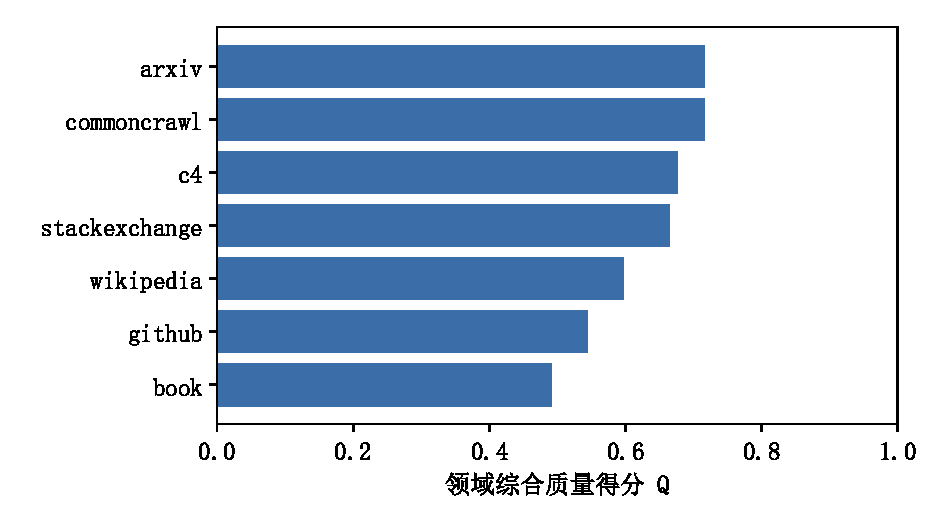
\includegraphics[width=0.92\textwidth]{figures/q1_fig02_domain_quality_scores.pdf}
          \caption{最终领域质量得分}
          \label{fig:qualitydomain}
        \end{figure}
        

        \subsubsection{A1 与扩展集的一致性}    % 4.3.2
        表~\ref{tab:extension}显示，arxiv 扩展集的平均质量比 A1 抽样低 0.00604，Cohen's $d=-0.0700$；github 的均值差仅 $-0.00126$，Cohen's $d=-0.0144$。arxiv 的 KS 检验因样本量大而达到统计显著，但效应量很小，不能据此声称抽样集与扩展集存在实质性质量差异。github 的分布差异也很小。扩展结果支持 A1 对这两个领域的均值代表性。
        
        \begin{table}[H]
        \centering
        \caption{A1 抽样与扩展集质量对照} % table 4.3
        \label{tab:extension}
        \begin{tabular}{lrrrrrr}
        \toprule
        领域 & $n_{A1}$ & $n_{ext}$ & $Q_{A1}$ & $Q_{ext}$ & 均值差 & Cohen's $d$ \\
        \midrule
        arxiv & 1,419 & 17,523 & 0.72287 & 0.71684 & $-0.00604$ & $-0.0700$ \\
        github & 10,000 & 203,752 & 0.54596 & 0.54470 & $-0.00126$ & $-0.0144$ \\
        \bottomrule
        \end{tabular}
        \end{table}
        
        % \begin{figure}[H]
        %   \centering
        %   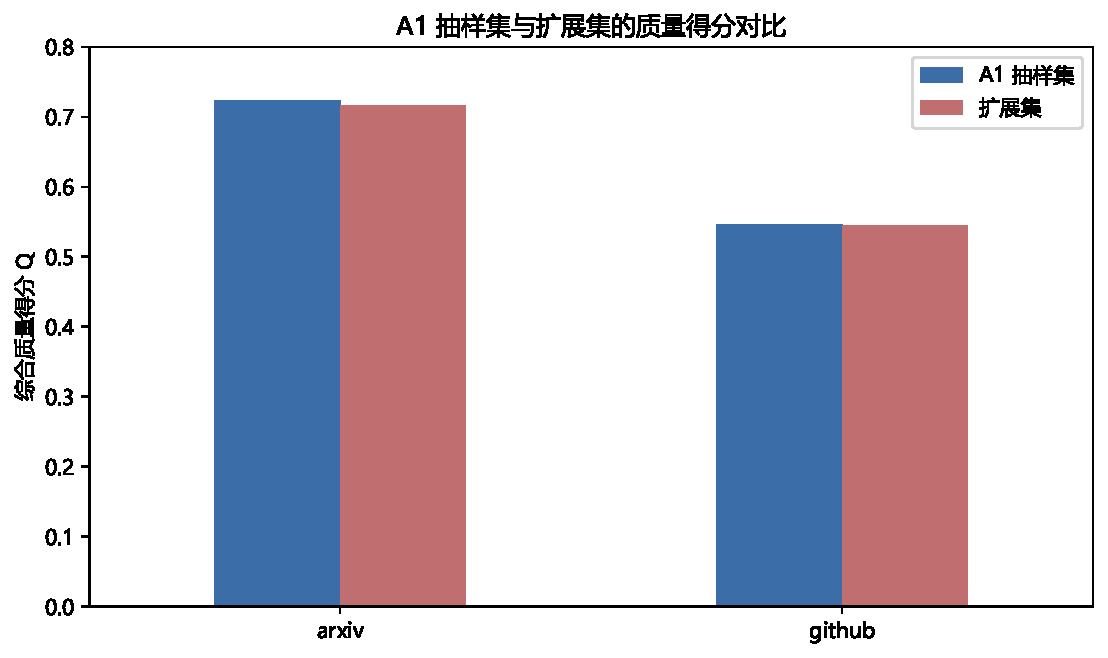
\includegraphics[width=0.80\textwidth]{figures/q1_fig03_extension_quality_comparison.pdf}
        %   \caption{A1 抽样与 A2/A3 扩展集平均质量比较}
        %   \label{fig:extension}
        % \end{figure}


        \subsubsection{冲突结构与消解结果}  % 4.3.3
        全体 272,505 条记录的冲突率为 7.675\%。冲突贡献最高的指标为数字字符比例、词数、最高频三元字符比例、句数、最高频二元字符比例和广告信号，归一化贡献分别为 0.0617、0.0607、0.0569、0.0542、0.0538 和 0.0523。该结果说明冲突主要来自文本结构、长度和重复特征与模型型质量分之间的分歧，而非某个单一指标完全失效。
        
        \begin{figure}[H]
          \centering
          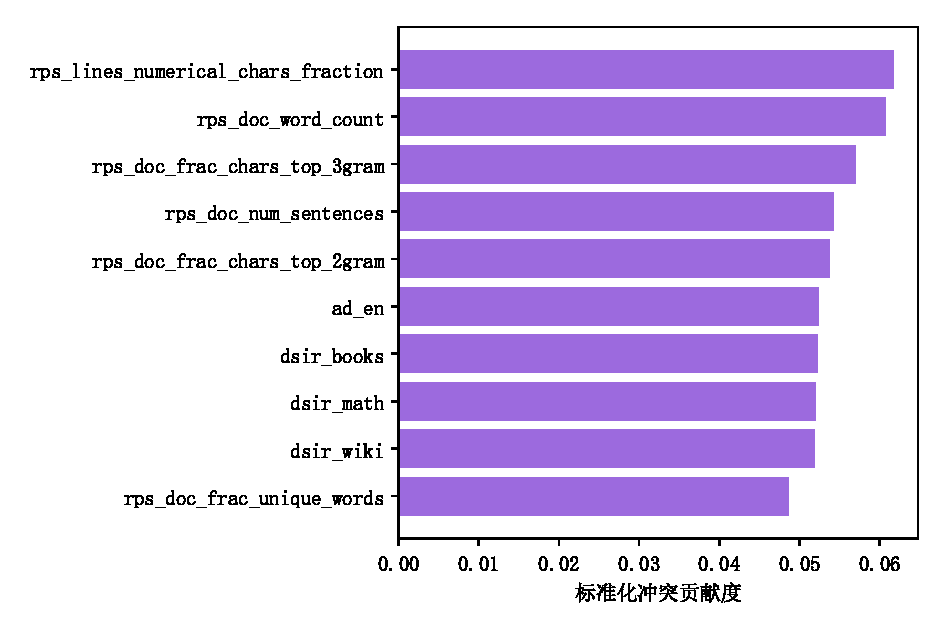
\includegraphics[width=0.93\textwidth]{figures/q1_fig04_conflict_metric_contributions.pdf}
          \caption{质量冲突的主要指标来源}
          \label{fig:conflictcontrib}
        \end{figure}
        
        Huber 聚合在冲突样本中降低大残差指标的有效权重，同时保留文本记录和其余指标。相比``检测冲突后删除样本''，该处理不会系统性排除包含公式、代码或特殊格式的高价值文本。置信度 $Conf_i$ 则将分歧程度和原始覆盖率显式保留下来，便于后续模型使用质量分时进行筛选或加权。


        \subsubsection{配比模型验证} % 4.3.4
        表~\ref{tab:validation}给出三组真实检验结果。1M 同规模检验取得 RMSE 0.28465、MAE 0.20269、$R^2=0.86473$，平均 Spearman 为 0.93396，说明二次 ILR 岭回归能够同时解释多数验证域的配比差异。

        为进一步考察模型在各验证域上的预测表现，图~\ref{fig:q1_ridge_loss_curves} 给出了 1M 同规模检验集中 256 个配方对应的 13 个 Loss 目标的预测结果。灰色散点表示实测 Loss，红色曲线表示二次 ILR 岭回归的预测值。每个子图按相应目标的预测值升序排列，并对实测值作相同重排；因此，横轴表示排序后的配方序号，不代表某一领域的配比，各子图的排序也不必相同。图中预测直接来自训练集上拟合的模型，未使用检验标签进行重新拟合、校准或额外平滑。

        13 个验证域的 $R^2$ 均超过 0.81，范围为 0.81375--0.91014。其中，uspto\_backgrounds 的 $R^2=0.91014$，freelaw 和 wikipedia\_en 分别为 0.90486 和 0.90342，表明模型在这些验证域上能够较好地刻画配方变化对应的损失差异。dm\_mathematics 的 RMSE 为 0.56226，高于其他验证域，但其 $R^2$ 仍达到 0.86555，说明预测误差在不同验证域间存在差异；比较绝对误差时，还应结合各域 Loss 的变化范围。

        \begin{figure}[p]
          \centering
          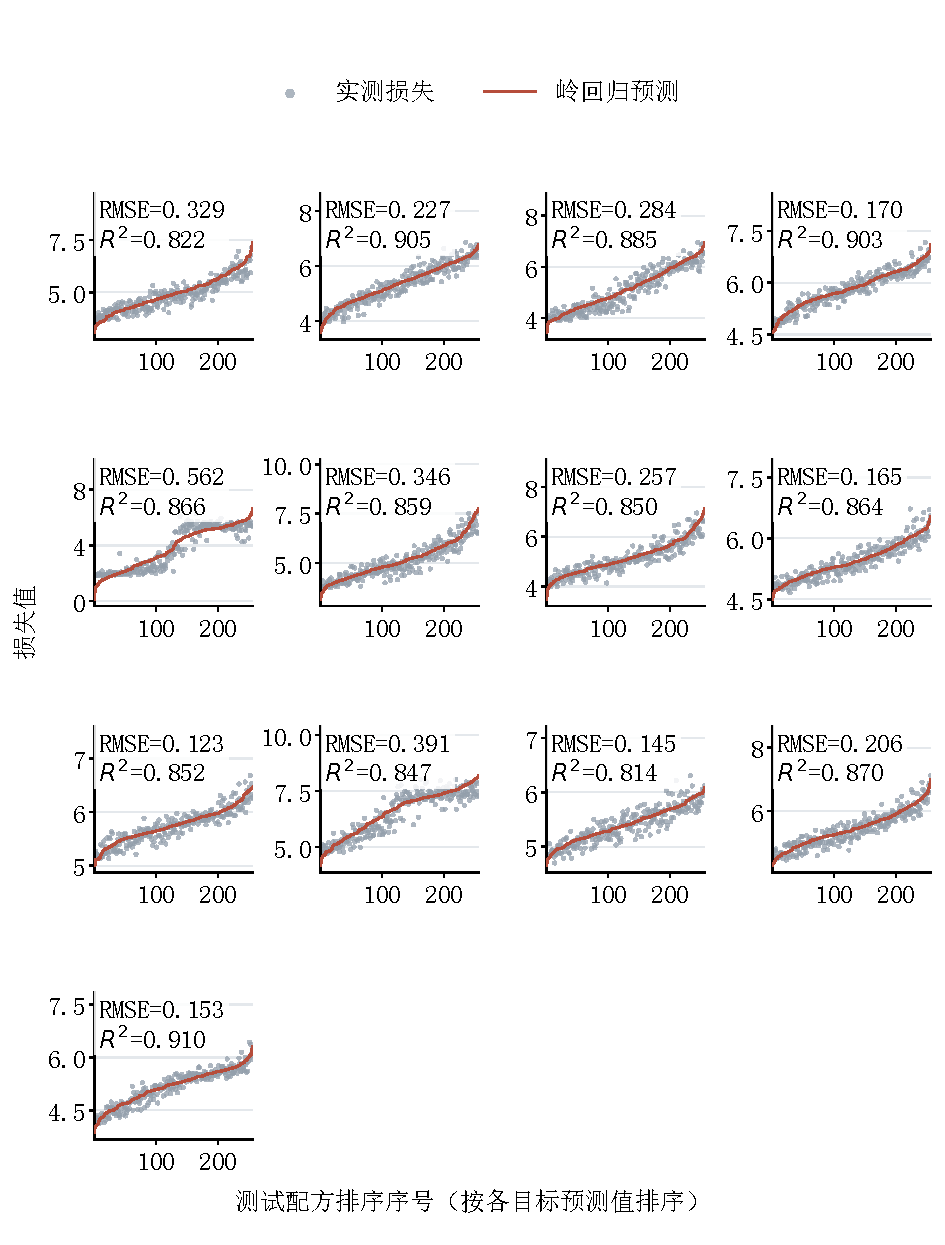
\includegraphics[width=\textwidth]{figures/q1_fig09_ridge_loss_curves.pdf}
          \caption{1M 同规模检验集上 13 个 Loss 目标的岭回归预测与实测值}
          \label{fig:q1_ridge_loss_curves}
        \end{figure}
        
        60M 和 1B 的未校准 $R^2$ 为负，原因是模型规模改变了绝对 Loss 基准，而非配方排序失效。二者的平均 Spearman 仍为 0.92950 和 0.84253。使用检验标签做每个目标的一维仿射校准后，$R^2$ 分别达到 0.85178 和 0.81292；该结果只说明单调结构可通过尺度和平移校准，不视为独立预测性能。
        
        \begin{table}[H]
        \centering
        \caption{A6--A11 配比模型验证结果}  % table 4.4
        \label{tab:validation}
        \begin{threeparttable}
        \begin{tabular}{lrrrrrr}
        \toprule
        检验集 & RMSE & MAE & $R^2$ & 平均 Spearman & 校准 RMSE & 校准 $R^2$ \\
        \midrule
        1M & 0.28465 & 0.20269 & 0.86473 & 0.93396 & 0.27409 & 0.87458 \\
        60M & 1.59999 & 1.50659 & $-7.30804$ & 0.92950 & 0.21371 & 0.85178 \\
        1B & 2.70008 & 2.62433 & $-189.99642$ & 0.84253 & 0.08450 & 0.81292 \\
        \bottomrule
        \end{tabular}
        \begin{tablenotes}\small
        \item 注：60M、1B 的仿射校准使用相应检验标签，只用于描述跨规模单调迁移，不是独立预测。
        \end{tablenotes}
        \end{threeparttable}
        \end{table}
        
        % \begin{figure}[H]   % figure 4.5
        %   \centering
        %   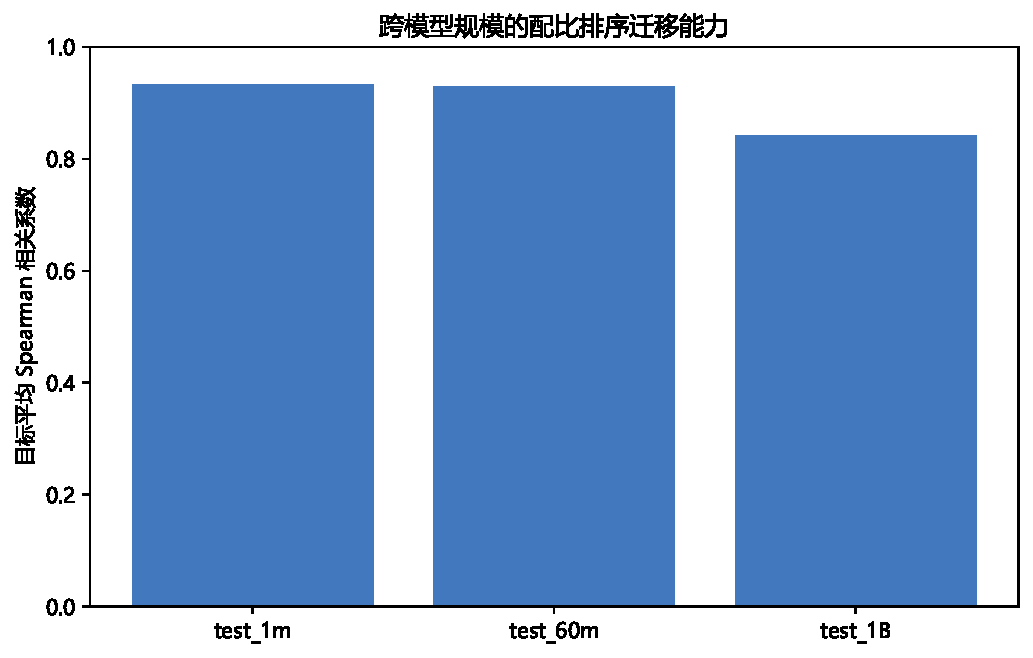
\includegraphics[width=0.78\textwidth]{figures/q1_fig05_mixture_validation_spearman.pdf}
        %   \caption{不同参数规模下的配方排序迁移}
        %   \label{fig:spearman}
        % \end{figure}


        \subsubsection{领域主效应} % 4.3.5
        图~\ref{fig:maineffect}展示在 200 个训练配方附近计算的平均局部导数。dm\_mathematics、ubuntu\_irc、stackexchange 的平均导数分别为 $-7.216$、$-6.711$、$-6.515$，即增加 1 个百分点份额时，平均 Loss 的预测变化约为 $-0.0722$、$-0.0671$、$-0.0651$。enron\_emails、europarl 和 gutenberg\_pg\_19 的导数为正。由于不同参考配方下的导数标准差较大，这些数值应理解为样本分布上的平均局部关联。
        
        \begin{table}[H]
        \centering
        \caption{绝对值较大的领域局部边际效应}    % table 4.5    
        \label{tab:effects}
        \begin{tabular}{lrrl}
        \toprule
        领域 & $ME_k$ & 标准差 & 局部解释 \\
        \midrule
        dm\_mathematics & $-7.216$ & 7.897 & 增加份额通常降低 Loss \\
        ubuntu\_irc & $-6.711$ & 7.256 & 增加份额通常降低 Loss \\
        stackexchange & $-6.515$ & 9.119 & 增加份额通常降低 Loss \\
        enron\_emails & 5.354 & 14.464 & 增加份额通常提高 Loss \\
        freelaw & $-3.545$ & 8.092 & 增加份额通常降低 Loss \\
        arxiv & $-3.160$ & 6.573 & 增加份额通常降低 Loss \\
        github & $-3.139$ & 7.928 & 增加份额通常降低 Loss \\
        europarl & 2.252 & 8.100 & 增加份额通常提高 Loss \\
        \bottomrule
        \end{tabular}
        \end{table}
        
        \begin{figure}[H]
          \centering
          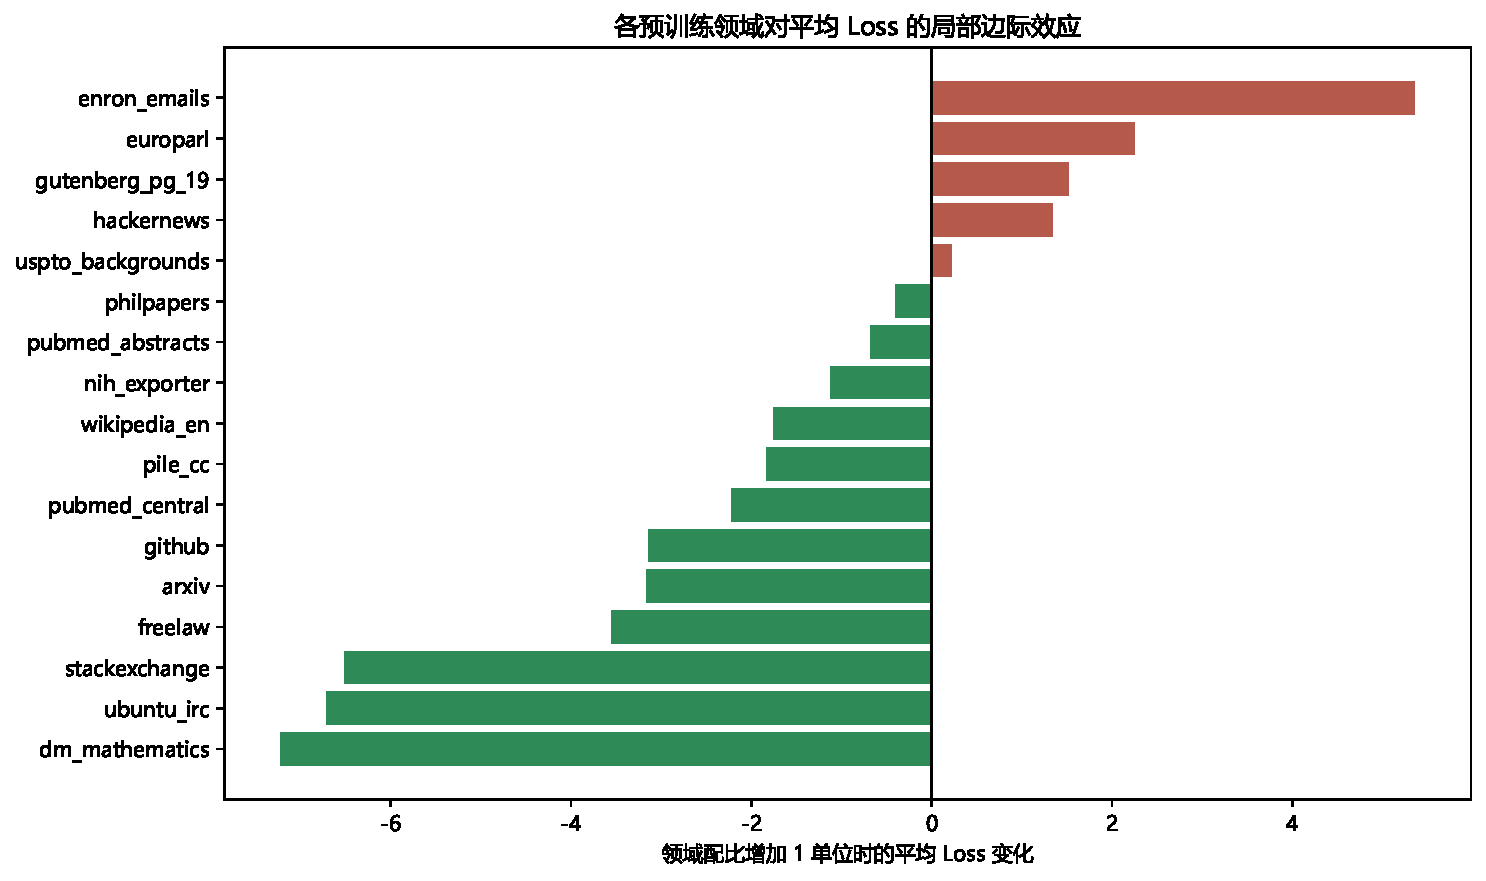
\includegraphics[width=0.96\textwidth]{figures/q1_fig06_mixture_domain_effects.pdf}
          \caption{17 个训练领域对平均 Loss 的局部边际效应}
          \label{fig:maineffect}
        \end{figure}


        \subsubsection{领域组合效应} % 4.3.6
        二阶差分绝对值最大的组合多涉及样本中较稀疏的 philpapers、nih\_exporter 和 enron\_emails。例如 philpapers--enron\_emails 的 $INT=87.85$，表示组合效果弱于主效应可加预期；enron\_emails--europarl 的 $INT=-18.33$，表现为局部协同。由于二阶效应对配方位置和伪计数更敏感，本文只把其作为筛选需要进一步实验的领域组合，不把数值直接解释为稳定因果效应。
        
        \begin{table}[H]
        \centering
        \caption{绝对值最大的领域组合效应}  % table 4.6
        \label{tab:interactions}
        \begin{tabular}{llrr}
        \toprule
        领域 1 & 领域 2 & $INT_{jk}$ & 类型 \\
        \midrule
        philpapers & enron\_emails & 87.85 & 拮抗 \\
        nih\_exporter & philpapers & 59.38 & 拮抗 \\
        nih\_exporter & enron\_emails & 51.52 & 拮抗 \\
        enron\_emails & hackernews & 44.71 & 拮抗 \\
        philpapers & europarl & 27.07 & 拮抗 \\
        enron\_emails & europarl & $-18.33$ & 协同 \\
        enron\_emails & gutenberg\_pg\_19 & 17.38 & 拮抗 \\
        nih\_exporter & europarl & 13.44 & 拮抗 \\
        \bottomrule
        \end{tabular}
        \end{table}


        \subsubsection{质量映射覆盖与不可辨识性}    % 4.3 7
        A16 的直接或近直接映射只覆盖 6 个配方域。训练配方中，已映射领域份额的平均值为 0.5646，即平均有 56.46\% 的语料份额能够对应到已有质量评分，1M/60M 检验为 0.5690，1B 为 0.6224；不同配方的覆盖质量从接近 0 到 1 不等。训练集的 $Q_{mix}$ 部分识别区间平均宽度为 0.0983，1M/60M 为 0.0973，1B 为 0.0852。该宽度表明，对未映射 11 域强行填入单一质量分会制造不可忽略的模型确定性。本文因此保留上下界，并将 $Q_{mix}^{mid}$ 只作为敏感性描述量。
        
        \begin{table}[H]
        \centering
        \caption{配方质量映射覆盖情况}    % table 4.7
        \label{tab:mapping}
        \begin{tabular}{lrrrr}
        \toprule
        数据集 & 样本量 & 已映射领域份额均值 & 已映射领域份额范围 & 平均区间宽度 \\
        \midrule
        训练 1M & 512 & 0.5646 & 0.000--1.000 & 0.0983 \\
        检验 1M & 256 & 0.5690 & 0.001--1.000 & 0.0973 \\
        检验 60M & 256 & 0.5690 & 0.001--1.000 & 0.0973 \\
        检验 1B & 64 & 0.6224 & 0.138--0.888 & 0.0852 \\
        外推 10B/70B & 各 63 & 0.5435 & 0.003--1.000 & 0.1030 \\
        \bottomrule
        \end{tabular}
        \end{table}


        \subsubsection{外推稳定性}   % 4.3.8
        A12--A15 上的未校准绝对误差很大，符合模型规模改变 Loss 基准的预期。10B 和 70B 的配方排序平均 Spearman 分别为 0.60949 和 0.52874；使用外推标签做仿射校准后 $R^2$ 分别为 0.57882 和 0.45793。该结果说明效应排序具有中等稳定性，但明显弱于真实 60M/1B 检验。由于外推配比为训练子集、Loss 也来自外推，本文不把它作为真实大模型实验验证。
        
        \begin{table}[H]
        \centering
        \caption{A12--A15 外推稳定性结果}  % table 4.8
        \label{tab:extrapolation}
        \begin{tabular}{lrrrr}
        \toprule
        数据集 & 未校准 RMSE & 平均 Spearman & 校准 RMSE & 校准 $R^2$ \\
        \midrule
        10B 外推 & 3.62349 & 0.60949 & 0.17124 & 0.57882 \\
        70B 外推 & 4.01115 & 0.52874 & 0.16192 & 0.45793 \\
        \bottomrule
        \end{tabular}
        \end{table}


        \subsubsection{小结}  % 4.3.9
        本节完成了问题一的质量评价、冲突消解和领域配比建模。基于 272,505 条记录构建的 Huber 综合质量分能够统一 22 个异质指标。arxiv 与 commoncrawl 的领域质量最高，github 与 book 较低；book 的样本量和冲突结构使其不确定性更大。总体冲突率为 7.675\%。冲突主要与数字比例、文本长度和重复统计有关。Huber 估计能够在不删除文本的情况下抑制离群指标。arxiv、github 的扩展集与 A1 抽样集平均质量差异很小，Cohen's $d$ 的绝对值均小于 0.08，支持 A1 的均值代表性ILR 二次岭回归在 1M 检验集上达到 $R^2=0.86473$，跨到 60M 和 1B 后配方排序相关仍为 0.92950 和 0.84253。配比规律主要以相对排序形式迁移，绝对 Loss 需要规模校准在观测配方邻域内，dm\_mathematics、ubuntu\_irc、stackexchange 的平均边际效应最有利；enron\_emails 的平均效应不利。该结论仅适用于局部调整。A16 的映射覆盖不足以识别独立质量系数。部分识别区间比主观补值更诚实，也为问题二引入质量因素提供了不确定性边界。


\section{问题二}   % 5
    \subsection{问题分析}
    质量评分、领域配比和模型规模来自不同的实验体系，不能将全部 Loss 记录直接拼接后回归。一方面，问题一的质量映射只覆盖部分训练领域，其余领域只能给出条件区间；另一方面，质量代表值本身是配比的线性组合，如果同时将质量代表值和全部份额作为自由解释变量，难以识别独立质量作用。因此，本问沿用问题一的质量与配比结果，将“改变配方”和“固定配方后额外改善质量”分开建模。

    规模信息由 B1 的训练轨迹提供，质量响应主要由 B6 中固定参数量、数据量后改变质量的记录提供。B6 的半合成性质以及不同来源的评价口径差异，决定了质量响应系数 $\gamma$ 只能作为条件迁移参数，不能直接解释为真实训练中的统一规律。B7 还包含与 B6 重复的记录，必须先去重再检验；插值和估算数据只用于一致性分析。

    参考计算最优训练的双幂律框架\textsuperscript{\cite{hoffmann2022chinchilla}}以及数据配比与训练规模相衔接的研究思路\textsuperscript{\cite{ye2025mixing}}，本文采用“经典标度律参数估计、质量响应系数估计、配比相对响应修正”的分阶段建模方法。以双幂律刻画参数量和训练数据量的影响，用当前配方与参考配方的平均预测 Loss 之比表示配比响应，再通过正值修正因子将额外质量改善接入模型。模型建立后，利用留出检验与跨来源比较确定适用范围，并推导边际收益、质量与参数的等效替代条件，以及单纯形内的领域局部交互关系。

    \subsection{模型建立}
        \subsubsection{数据整理与问题一结果衔接}  % 5.2.1
        以验证集交叉熵损失 $L$ 为评价指标，数值越小表示预测性能越好。为统一数量级，记
        \begin{equation}
         n=\frac{N}{10^9},\qquad d=\frac{D}{10^{11}},\qquad
         \bm p=(p_1,\ldots,p_{17})^\mathsf T,\quad
         p_j\geq0,\quad\sum_{j=1}^{17}p_j=1.
         \label{eq:p2_units}
        \end{equation}
        其中，$n=7,d=3$ 分别对应 70 亿参数与 3000 亿 tokens。对附件中的配比先归一化，使各领域份额之和等于 1，再调用问题一的预测模型。
        
        问题一的接口包括领域质量、512 个训练配方及其已拟合的配比模型。这里的一个配方是由 17 个领域份额组成的向量，512 个配方对应 512 种训练语料混合方案。取这些配方的算术均值为参考配比 $\bm p_0$。质量数据与配方数据的领域分类并不完全对应，仅有 6 个配方域能够直接或近似映射，其余 11 个域沿用问题一的敏感性代表值，即全局加权质量均值 $q_G$，构造可计算的常规质量基准。设可映射领域集合为 $M$，定义配方的常规质量为
        \begin{equation}
         \bar q_j=\begin{cases}q_j,&j\in M,\\q_G,&j\notin M,\end{cases}
         \qquad \bar Q(\bm p)=\sum_{j=1}^{17}p_j\bar q_j,
         \qquad Q_0=\bar Q(\bm p_0)=0.610914.
         \label{eq:p2_quality}
        \end{equation}
        $Q_0$ 只用于归一化，不代表对 B1 训练语料质量的实际测量。该代表值并非新增的质量观测，也不取代问题一的部分识别区间；在敏感性分析中，将其取值范围设为已观测领域质量的最小值至最大值，得到条件性的配方质量区间。
        
        Pythia 提供在受控训练设置下的多规模模型及中间检查点，为分析训练规模与训练进程提供了实验背景\textsuperscript{\cite{biderman2023pythia}}。本研究的具体观测及其证据性质以赛事附件和数据说明为准。规模参数主要由 B1 的 1176 个训练检查点估计，覆盖 8 个参数规模；质量响应由 B6 的 360 条半合成记录估计。B7 的 450 条记录中有 360 条与 B6 完全重合，故只保留其余 90 条用于新质量水平验证。B3 为基于 B1 生成的插值数据，B10 为估算损失，二者均不作为新增真实实验。B2、B4、B5 用于跨来源迁移检验，B8 用于质量方向的一致性审查。对 B9 排除 4 条规模缺失或非正的记录，其余 128 条仅用于大模型情景预测。
    
        \subsubsection{经典标度律}  % 5.2.2
        借鉴 Hoffmann 等提出的参数量与训练数据量双幂律形式\textsuperscript{\cite{hoffmann2022chinchilla}}，以参数受限和数据受限造成的超额损失构造规模基准，并使用附件 B 重新估计系数和指数：
        \begin{equation}
         L_0(n,d)=E+A n^{-\alpha}+B d^{-\beta},\qquad
         X=A n^{-\alpha},\quad Y=B d^{-\beta}.
         \label{eq:p2_baseline}
        \end{equation}
        其中 $E\geq0$ 为该模型下的渐近损失水平，$A,B>0$ 决定两类超额损失的幅度，$\alpha,\beta>0$ 表示规模增长的衰减速度。因而 $X$ 和 $Y$ 均随相应资源增加而减小。
        
        \subsubsection{质量与配比修正因子}  % 5.2.3
        在 RegMix 的配比性能代理预测思路基础上\textsuperscript{\cite{liu2025regmix}}，复用问题一采用 ILR 坐标与岭正则化构建的二次回归模型\textsuperscript{\cite{egozcue2003ilr,hoerl1970ridge}}，将 13 个验证域的预测损失取算术平均，记为 $f_A(\bm p)$。为避免直接叠加不同评价口径下的绝对损失，使用相对响应
        \begin{equation}
         f_A(\bm p)=\frac1{13}\sum_{r=1}^{13}\widehat L_{A,r}(\bm p),
         \qquad h(\bm p)=\log\frac{f_A(\bm p)}{f_A(\bm p_0)}.
         \label{eq:p2_mix}
        \end{equation}
        于是 $h(\bm p_0)=0$，$h(\bm p)<0$ 表示该配方在问题一模型中优于参考配方。该定义要求所用配方的预测损失为正；本文在已计算的配方及参考点邻域内使用该响应。
        
        已有研究通过质量因子修正标度律的数据项\textsuperscript{\cite{subramanyam2026quality}}，为显式引入质量提供了参考；其质量定义与本文的综合评分并不等同。本文进一步假设，固定配比后的额外质量改善按比例减少参数项与数据项之和所构成的超额损失。下式中的指数质量修正、相对配比响应及其组合方式均为本文的建模设定，并通过对照检验与敏感性分析考察适用性。将两种响应结合，得到
        \begin{equation}
         \begin{aligned}
         G(Q,\bm p)&=\exp\!\left\{\gamma\kappa[\bar Q(\bm p)-Q]+\lambda_p h(\bm p)\right\},\\
         L(n,d,Q,\bm p)&=E+\left(A n^{-\alpha}+B d^{-\beta}\right)G(Q,\bm p).
         \end{aligned}
         \label{eq:p2_general}
        \end{equation}
        其中 $\gamma\geq0$ 为质量响应系数，$\kappa$ 表示附件 A 与 B 的质量尺度换算系数，$\lambda_p$ 表示配比效应的迁移强度。主情景设 $\kappa=\lambda_p=1$，并另行讨论其变化。现有附件不能唯一识别这两个迁移系数，故该设定属于模型假设。
        
        式\eqref{eq:p2_general}具有三个便于解释的性质。第一，在参考条件 $\bm p=\bm p_0,Q=Q_0$ 下，$G=1$，模型退化为式\eqref{eq:p2_baseline}。第二，改变配方且使用其常规质量，即 $Q=\bar Q(\bm p)$ 时，质量偏离项为零，已有的配方差异仅通过 $h(\bm p)$ 起作用，从而避免重复计入质量贡献。第三，固定规模与配比，将质量提高 $\Delta Q$ 后，有
        \begin{equation}
         \frac{L(n,d,Q+\Delta Q,\bm p)-E}{L(n,d,Q,\bm p)-E}
         =\exp(-\gamma\kappa\Delta Q),\qquad Q+\Delta Q\leq1.
         \label{eq:p2_qchange}
        \end{equation}
        这表示质量改善作用于可减少的损失部分，而不改变模型设定的渐近水平 $E$。
        
        \subsubsection{分阶段稳健参数估计}  % 5.2.4
        第一阶段，在 B1 上估计 $\bm\theta=(E,A,B,\alpha,\beta)$。由于同一规模下的后期检查点较密集，先将全局 $\log d$ 范围划为 8 个等宽区间，再使各规模、各非空区间获得均衡权重。若规模 $g$ 有 $K_g$ 个非空区间，区间 $(g,b)$ 内有 $m_{gb}$ 条记录，则原始权重为 $1/(K_gm_{gb})$，归一化后记为 $\omega_i$。令 $e_i(\bm\theta)=L_0(n_i,d_i)-L_i$，求解
        \begin{equation}
         \widehat{\bm\theta}=\arg\min_{\bm\theta}
         \sum_i\delta^2\left[\sqrt{1+\frac{\omega_i e_i(\bm\theta)^2}{\delta^2}}-1\right],
         \qquad \delta=0.1.
         \label{eq:p2_fit}
        \end{equation}
        该目标采用 Soft-L1 平滑鲁棒损失，在小残差附近接近平方损失，在大残差处减小异常值的影响。数值实现采用 SciPy 的 \texttt{least\_squares}，设置 \texttt{loss='soft\_l1'}，并通过多初值有界非线性最小二乘求解\textsuperscript{\cite{virtanen2020scipy}}。均衡权重、分阶段拟合及参数边界均为针对附件结构所作的实现选择。限制 $0\leq E<\min_iL_i$、$10^{-8}\leq A,B\leq30$、$0.005\leq\alpha,\beta\leq2$。
        
        第二阶段，固定第一阶段的指数，为 B6 设置独立的基线系数：
        \begin{equation}
         L_{6,i}=E_6+\left(A_6n_i^{-\widehat\alpha}+B_6d_i^{-\widehat\beta}\right)
         \exp\!\left\{\gamma(Q_0-Q_i)\right\}+\varepsilon_i.
         \label{eq:p2_fit_quality}
        \end{equation}
        仍采用稳健最小二乘，取 $\delta=0.05$，联合估计 $E_6,A_6,B_6,\gamma$。主模型只接收质量响应 $\gamma$，其规模基线仍采用 B1 的参数，从而允许 B1 与 B6 存在绝对损失差异。
    
        \subsubsection{验证设计与不确定性估计}  % 5.2.5
        在 B1 上分别实施按参数规模留出和按训练阶段留出。前者每次留出一个规模的完整训练轨迹，合并八次留出预测评价泛化误差；后者对各规模按数据量排序，以前 70\% 检查点拟合、后 30\% 检查点检验。B6 按完整 $(N,D)$ 组进行五折交叉验证，同组质量水平进入同一折，比较无质量项、共享规模指数和自由规模指数三类模型。
        
        预测误差采用
        \begin{equation}
         \operatorname{RMSE}=\sqrt{\frac1m\sum_{i=1}^{m}(L_i-\widehat L_i)^2}.
         \label{eq:p2_rmse}
        \end{equation}
        配比迁移则对 13 个验证域平均 Loss 的排序计算 Spearman 相关系数。该指标与问题一“先对各验证域计算相关系数再求平均”的指标不同，分别报告，避免混用。
        
        借鉴 Bootstrap 重抽样估计不确定性的思想\textsuperscript{\cite{efron1979bootstrap}}，考虑同一轨迹或实验组内记录的相关性，本文对 B1 按完整规模轨迹、对 B6 按完整 $(N,D)$ 组进行 200 次重采样，每次重新估计两阶段参数，并以 2.5\% 与 97.5\% 分位数构造条件 95\% 区间。质量量尺 $\kappa$ 和配比迁移强度 $\lambda_p$ 另行进行敏感性分析，不将这些结构假设的不确定性混入抽样区间。
    
        \subsubsection{边际收益与单位成本条件}  % 5.2.6
        令 $\eta=\gamma\kappa$，将增加单位资源带来的损失减少量定义为边际收益。固定其他变量，由式\eqref{eq:p2_general}可得
        \begin{equation}
         U_n=-\frac{\partial L}{\partial n}=\frac{\alpha XG}{n},\qquad
         U_d=-\frac{\partial L}{\partial d}=\frac{\beta YG}{d},\qquad
         U_Q=-\frac{\partial L}{\partial Q}=\eta(X+Y)G.
         \label{eq:p2_marginal}
        \end{equation}
        $U_n$ 对应每增加十亿参数的局部收益，$U_d$ 对应每增加一千亿 tokens 的局部收益，两者不能忽略单位直接比较。对超额损失 $F=L-E$，进一步定义无量纲的改进弹性：
        \begin{equation}
         \epsilon_n^F=\frac{\alpha X}{X+Y},\qquad
         \epsilon_d^F=\frac{\beta Y}{X+Y},\qquad
         \epsilon_Q^F=\eta Q.
         \label{eq:p2_elasticity}
        \end{equation}
        
        
        三种资源方向上的二阶导数均非负，参数量与数据量方向严格为正，表明模型具有边际收益递减特征。参数量与质量的混合导数为 $\eta\alpha XG/n\geq0$，意味着在本模型中，质量改善会降低继续扩容的边际降损收益，二者表现为局部替代。
        
        设增加十亿参数的边际成本为 $c_n>0$，提高一个质量单位的边际成本为 $c_Q>0$。比较 $U_n/c_n$ 与 $U_Q/c_Q$，得到优先改善质量的条件
        \begin{equation}
         \frac{c_Q}{c_n}<\frac{\eta n(X+Y)}{\alpha X}.
         \label{eq:p2_cost}
        \end{equation}
        附件未提供与该场景对应的真实货币成本，故本问给出临界成本比，不据此认定某一方案必然更便宜。若固定总训练算力 $C=6ND$，扩容会同时减少可用训练数据量，此时沿算力约束的收益变为 $G(\alpha X-\beta Y)/n$，只有 $\alpha X>\beta Y$ 时继续增加参数才有利。
    
        \subsubsection{质量提高与参数扩容的等效条件}  % 5.2.7
        固定数据量与配比，比较两种达到同样损失的方案：一是保持参数量 $n$，将质量从 $Q$ 提高至 $Q+\Delta Q$；二是保持原质量，将参数量提高至 $n_{\mathrm{eq}}$。令 $t=\exp(-\eta\Delta Q)$，消去相同的 $E$ 和原修正因子后，有
        \begin{equation}
         A n_{\mathrm{eq}}^{-\alpha}+Y=t(X+Y),\qquad
         \frac{n_{\mathrm{eq}}}{n}=\left[\frac{t(X+Y)-Y}{X}\right]^{-1/\alpha}.
         \label{eq:p2_equiv}
        \end{equation}
        有限等效扩容解要求 $t(X+Y)>Y$。当 $\eta>0$ 时，这一条件等价于
        \begin{equation}
         0<\Delta Q<\frac1\eta\log\left(1+\frac XY\right),\qquad Q+\Delta Q\leq1.
         \label{eq:p2_equiv_bound}
        \end{equation}
        当等式边界成立时，需要的参数量趋于无穷；超过该边界后，质量提升带来的目标损失已低于固定数据量下仅靠扩容所能达到的极限。因此，质量改善并不总能用有限参数扩容来等价替代。
    
        \subsubsection{领域边际作用与局部交互}  % 5.2.8
        由于配比之和固定，提高某个领域份额必须相应减少其他份额。本文固定参数量与数据量，在参考配比 $\bm p_0$ 附近分析，并沿 $Q=\bar Q(\bm p)$ 的常规质量路径改变配方。对单一领域 $j$，取 $v_{j,j}=1$，其余分量为 $v_{j,l}=-p_{0,l}/(1-p_{0,j})$，即其余领域按比例让出份额。计算方向导数 $D_{v_j}L$，负值表示这一局部调整能够降低平均损失。
        
        对领域 $j,k$ 的交互，使用其余 15 个领域组成的共同供给池。令 $\bm e_j$ 为第 $j$ 个单位向量，定义
        \begin{equation}
         u_l=\begin{cases}0,&l\in\{j,k\},\\
         \dfrac{p_{0,l}}{1-p_{0,j}-p_{0,k}},&l\notin\{j,k\},\end{cases}
         \qquad \bm v_j=\bm e_j-\bm u,\quad \bm v_k=\bm e_k-\bm u.
         \label{eq:p2_pool}
        \end{equation}
        将两个方向固定在参考点，记 $\ell(\bm p)=L(n,d,\bar Q(\bm p),\bm p)$，以步长 $\varepsilon_p=10^{-4}$ 的四角中心差分计算混合导数：
        \begin{equation}
         \begin{aligned}
         I_{jk}\approx\frac1{4\varepsilon_p^2}\big[&\ell(\bm p_0+\varepsilon_p\bm v_j+\varepsilon_p\bm v_k)
         -\ell(\bm p_0+\varepsilon_p\bm v_j-\varepsilon_p\bm v_k)\\
         &-\ell(\bm p_0-\varepsilon_p\bm v_j+\varepsilon_p\bm v_k)
         +\ell(\bm p_0-\varepsilon_p\bm v_j-\varepsilon_p\bm v_k)\big].
         \end{aligned}
         \label{eq:p2_interaction}
        \end{equation}
        $I_{jk}<0$ 表示增加一个领域会使另一个方向的边际降损作用增强，称为该路径下的局部互补；$I_{jk}>0$ 表示边际降损作用减弱，称为局部替代。

    \subsection{建模结果}
        \subsubsection{参数估计与规模拟合}  % 5.3.1
        表\ref{tab:p2_parameters}给出两阶段主参数及条件 Bootstrap 区间。所有估计均未落在数值求解边界上。区间只反映给定模型与数据生成方式下的抽样变化，不包含质量量尺和跨来源迁移假设的不确定性。

        \begin{table}[H]
         \centering
         \caption{广义标度律的参数估计}
         \label{tab:p2_parameters}
         \begin{tabular}{ccc}
          \toprule
          参数 & 点估计 & 条件 Bootstrap 95\% 区间 \\
          \midrule
          $E$ & 1.689482 & [1.688891, 1.690181] \\
          $A$ & 0.354064 & [0.353349, 0.354692] \\
          $B$ & 0.342016 & [0.341785, 0.342208] \\
          $\alpha$ & 0.339921 & [0.339433, 0.340627] \\
          $\beta$ & 0.279796 & [0.279714, 0.279893] \\
          $\gamma$ & 0.410160 & [0.389385, 0.433103] \\
          \bottomrule
         \end{tabular}
        \end{table}
        
        图\ref{fig:p2_scaling}展示了 B1 检查点与拟合曲线。图中散点为附件值，曲线为模型预测结果。随训练数据量增大，各参数规模下的损失逐渐下降，且下降幅度逐步减小；相同数据量下，较大模型通常对应较低损失。全量拟合的 RMSE 为 $1.522\times10^{-4}$，说明附件曲线与所设函数形式高度一致。
        
        \begin{figure}[H]
         \centering
         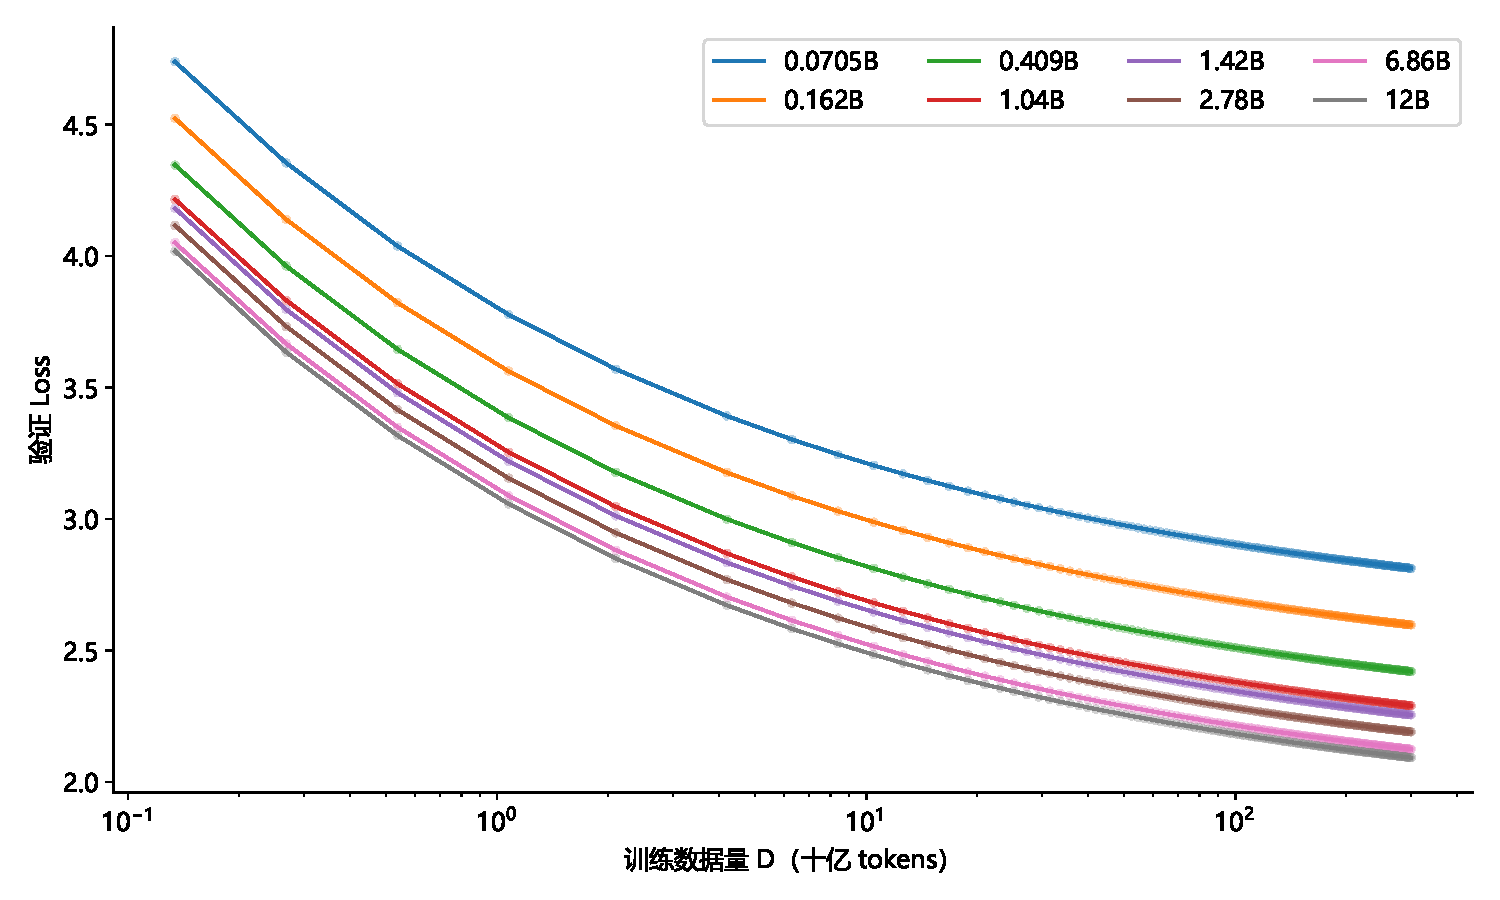
\includegraphics[width=\linewidth]{figures/q2_fig01_scaling_fit.pdf}
         \caption{B1 的训练检查点与经典标度律拟合}
         \label{fig:p2_scaling}
        \end{figure}

        \subsubsection{分层验证与质量项贡献}  % 5.3.2
        无质量项模型的平均 RMSE 为 0.129993，加入质量项后降至 0.054591，约降低 58.0\%；允许 B6 单独估计规模指数时进一步降至 0.052462。因此，质量项在该半合成数据内有效，但共享规模指数并非唯一可能的设定。上述对照分别检验质量项的贡献与规模指数共享假设。
        
        \begin{table}[H]
         \centering
         \caption{B6 质量项消融与共享指数检验}
         \label{tab:p2_quality_ablation}
         \begin{tabular}{lc}
          \toprule
          模型 & 五折分组验证平均 RMSE \\
          \midrule
          无质量项模型 & 0.129993 \\
          共享 B1 指数的质量模型 & 0.054591 \\
          自由指数质量模型 & 0.052462 \\
          \bottomrule
         \end{tabular}
        \end{table}
        
        主要检验结果见表\ref{tab:p2_validation}。B1 两类留出的误差均较小，但 B2 的直接迁移误差显著增大，B4 与 B5 也保留明显误差，说明仅使用同一组规模参数不足以消除来源间的评价口径差异。尤其是 B1 的误差已接近附件的数值舍入精度，不能据此推断任意真实训练实验都会达到同样精度。
        
        \begin{table}[H]
         \centering
         \caption{分层检验结果及其证据性质}
         \label{tab:p2_validation}
         \begin{tabularx}{\linewidth}{@{}l r >{\raggedright\arraybackslash}X@{}}
          \toprule
          检验方式 & RMSE & 解释范围 \\
          \midrule
          B1 留出参数规模 & 0.000181 & 同来源的未参与拟合规模 \\
          B1 留出后期检查点 & 0.000143 & 同来源的后期训练阶段 \\
          B2 直接迁移 & 1.243161 & 半合成数据，迁移误差较大 \\
          B3 轨迹比较 & 0.003799 & B1 派生插值的一致性 \\
          B4 跨模型族迁移 & 0.292703 & 跨来源记录，损失口径未统一 \\
          B5 文献数据迁移 & 0.197572 & 公开结果的有限迁移检验 \\
          B7 去重新增点 & 0.043803 & 90 个半合成的新质量水平 \\
          B8 直接预测 & 1.350759 & 质量方向冲突检验 \\
          B10 估算值比较 & 0.001049 & 估算机制的一致性 \\
          \bottomrule
         \end{tabularx}
        \end{table}
        
        \subsubsection{质量方向冲突}  % 5.3.3
        进一步固定 $(N,D)$ 检查质量变化方向。B6 的 45 个组中，质量与损失的线性趋势斜率均为负；B8 的 150 个组则全部为正。图\ref{fig:p2_conflict}将各组损失减去组内均值，以突出这种方向差异。图中每条折线对应固定的 $(N,D)$ 组，纵轴为组内中心化损失。因此，B8 与主模型的单调质量假设冲突，不纳入质量收益估计，也不通过反转质量分数来消除冲突。该结果限定了主模型的适用范围：质量改善结论以 B6 的质量定义和变化机制能够迁移为前提。
        
        \begin{figure}[H]
         \centering
         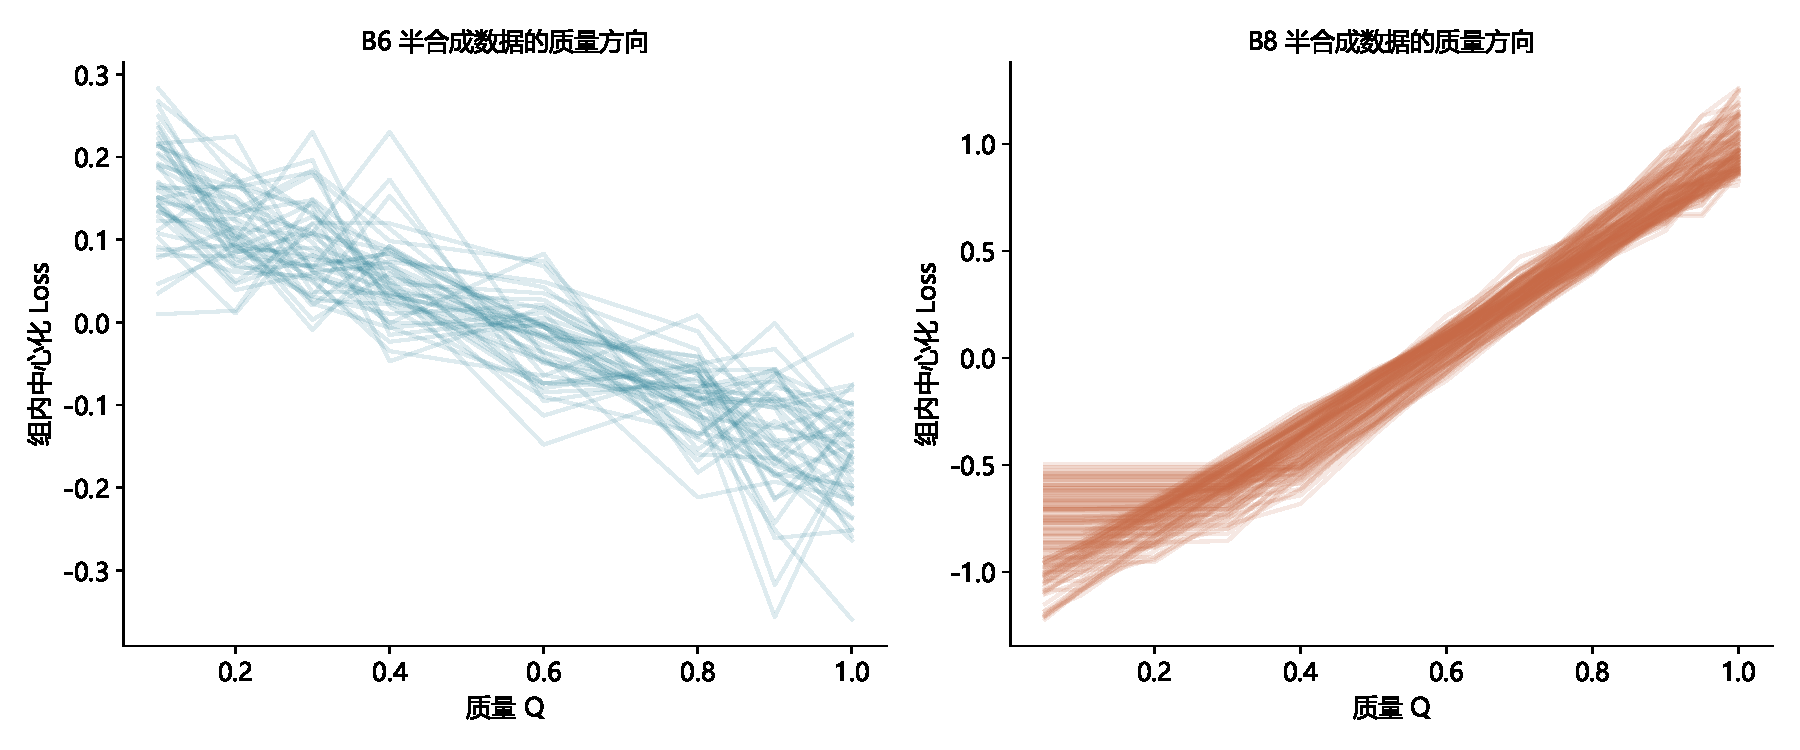
\includegraphics[width=\linewidth]{figures/q2_fig02_quality_direction_conflict.pdf}
         \caption{B6 与 B8 的质量方向比较}
         \label{fig:p2_conflict}
        \end{figure}
        
        \subsubsection{边际收益与成本比较}  % 5.3.4
        在 $n=7, d=3, \bm p=\bm p_0, Q=Q_0$ 的主情景下，超额 Loss 关于参数量、数据量和质量的改进弹性分别为 0.1430、0.1621 和 0.2506。例如，参数量局部增加 1\%，对应超额损失约减少 0.143\%。由于 $Q$ 是有界综合评分，质量改善还需结合式\eqref{eq:p2_qchange}中的绝对增量解释。
        
        在相同参考条件下，每增加 1B 参数的边际降损收益约为 0.008874，每增加 1B tokens 的收益约为 0.000235，提高一个质量单位的收益约为 0.178108。以上均为局部导数，质量提高 0.1 的有限变化仍应采用式\eqref{eq:p2_qchange}计算。
        
        式\eqref{eq:p2_cost}给出的临界成本比为 20.0718。由于缺少清洗筛选成本和对应训练成本，现有数据尚不能用于估计具体的货币节省金额。该条件为后续在成本约束下比较扩容、增加数据和改善质量提供接口。
        
        \subsubsection{质量提升的等效扩容结果}  % 5.3.5
        取 $N=7$B、$D=300$B、$\bm p=\bm p_0$，质量由 0.610914 提高至 0.710914。主情景的计算结果为
        \begin{equation}
         \begin{aligned}
         L_{\mathrm{before}}&=2.123722,\qquad L_{\mathrm{after}}=2.106271,\\
         N_{\mathrm{eq}}&=9.404464\text{B},\qquad N_{\mathrm{eq}}/N=1.343495.
         \end{aligned}
         \label{eq:p2_example}
        \end{equation}
        即质量提高 0.1 所带来的预测改进，约等价于增加 34.35\% 的参数。扩容倍数的条件 Bootstrap 95\% 区间为 $[1.322870,1.366724]$。该例是模型计算结果，并非真实对照实验；300B tokens 也略高于 B1 的最大值 299.893B，属于范围边缘的轻微外推。
        
        图\ref{fig:p2_equiv}给出不同起始规模和数据量下的等效扩容倍数。竖虚线为 B1 最大参数量 11.966B；$D=1000$B 曲线及等效参数超出 B1 范围的点同样涉及外推。固定数据量时，起始模型越大，参数受限项 $X$ 越小，同等质量改善对应的扩容倍数越高；增加数据量会降低数据受限项 $Y$，使相应倍数下降。超过 B1 支持范围的部分仅解释为条件外推。
        
        \begin{figure}[H]
         \centering
         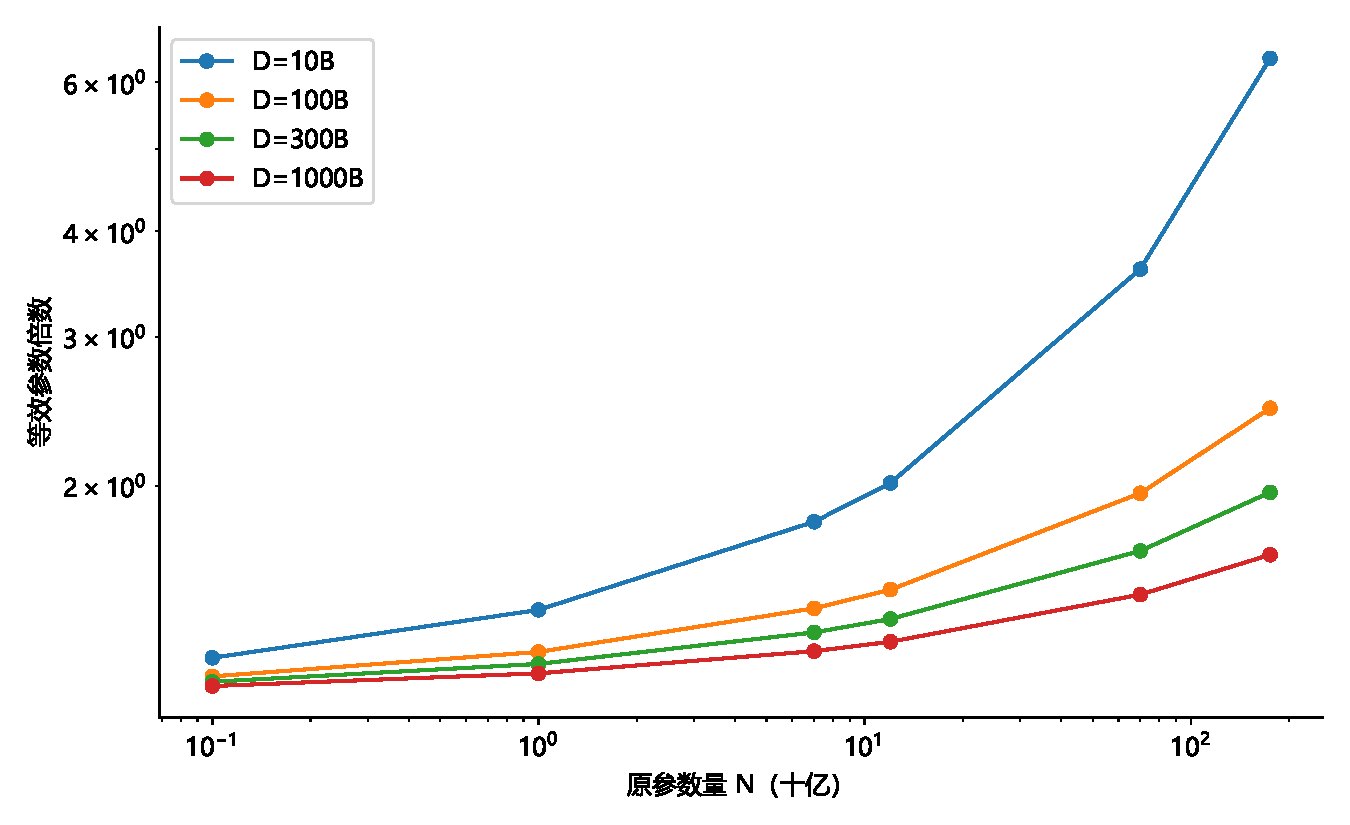
\includegraphics[width=\linewidth]{figures/q2_fig03_quality_parameter_equivalence.pdf}
         \caption{质量提高 0.1 的等效参数扩容倍数（$\kappa=1$）}
         \label{fig:p2_equiv}
        \end{figure}

        \subsubsection{领域主效应与组合关系}  % 5.3.6
        取 $N=7$B、$D=300$B、$\bm p=\bm p_0$，沿常规质量路径计算领域效应。
        
        dm\_mathematics、ubuntu\_irc 和 stackexchange 领域的方向导数分别为 $-0.116345$、$-0.099070$ 和 $-0.020586$。例如，在足够小且可行的邻域内，dm\_mathematics 领域份额增加一个百分点对应的损失变化约为 $-0.001163$。这些数值描述指定让出方式下的局部效应，不能直接推断大幅改变配方的收益。
        
        图\ref{fig:p2_interaction}给出各领域对的结果。enron\_emails 与 europarl 的混合导数为 $-6.861304$，表现为局部互补；philpapers 与 enron\_emails 的混合导数为 $32.483430$，表现为局部替代。不过，交互符号本身不能证明同时增加两个领域就能改善性能，还必须结合各自的一阶效应。低占比领域的结果尤其依赖参考配方及扰动方式，故这些关系不解释为普适因果关系。
        
        \begin{figure}[H]
         \centering
         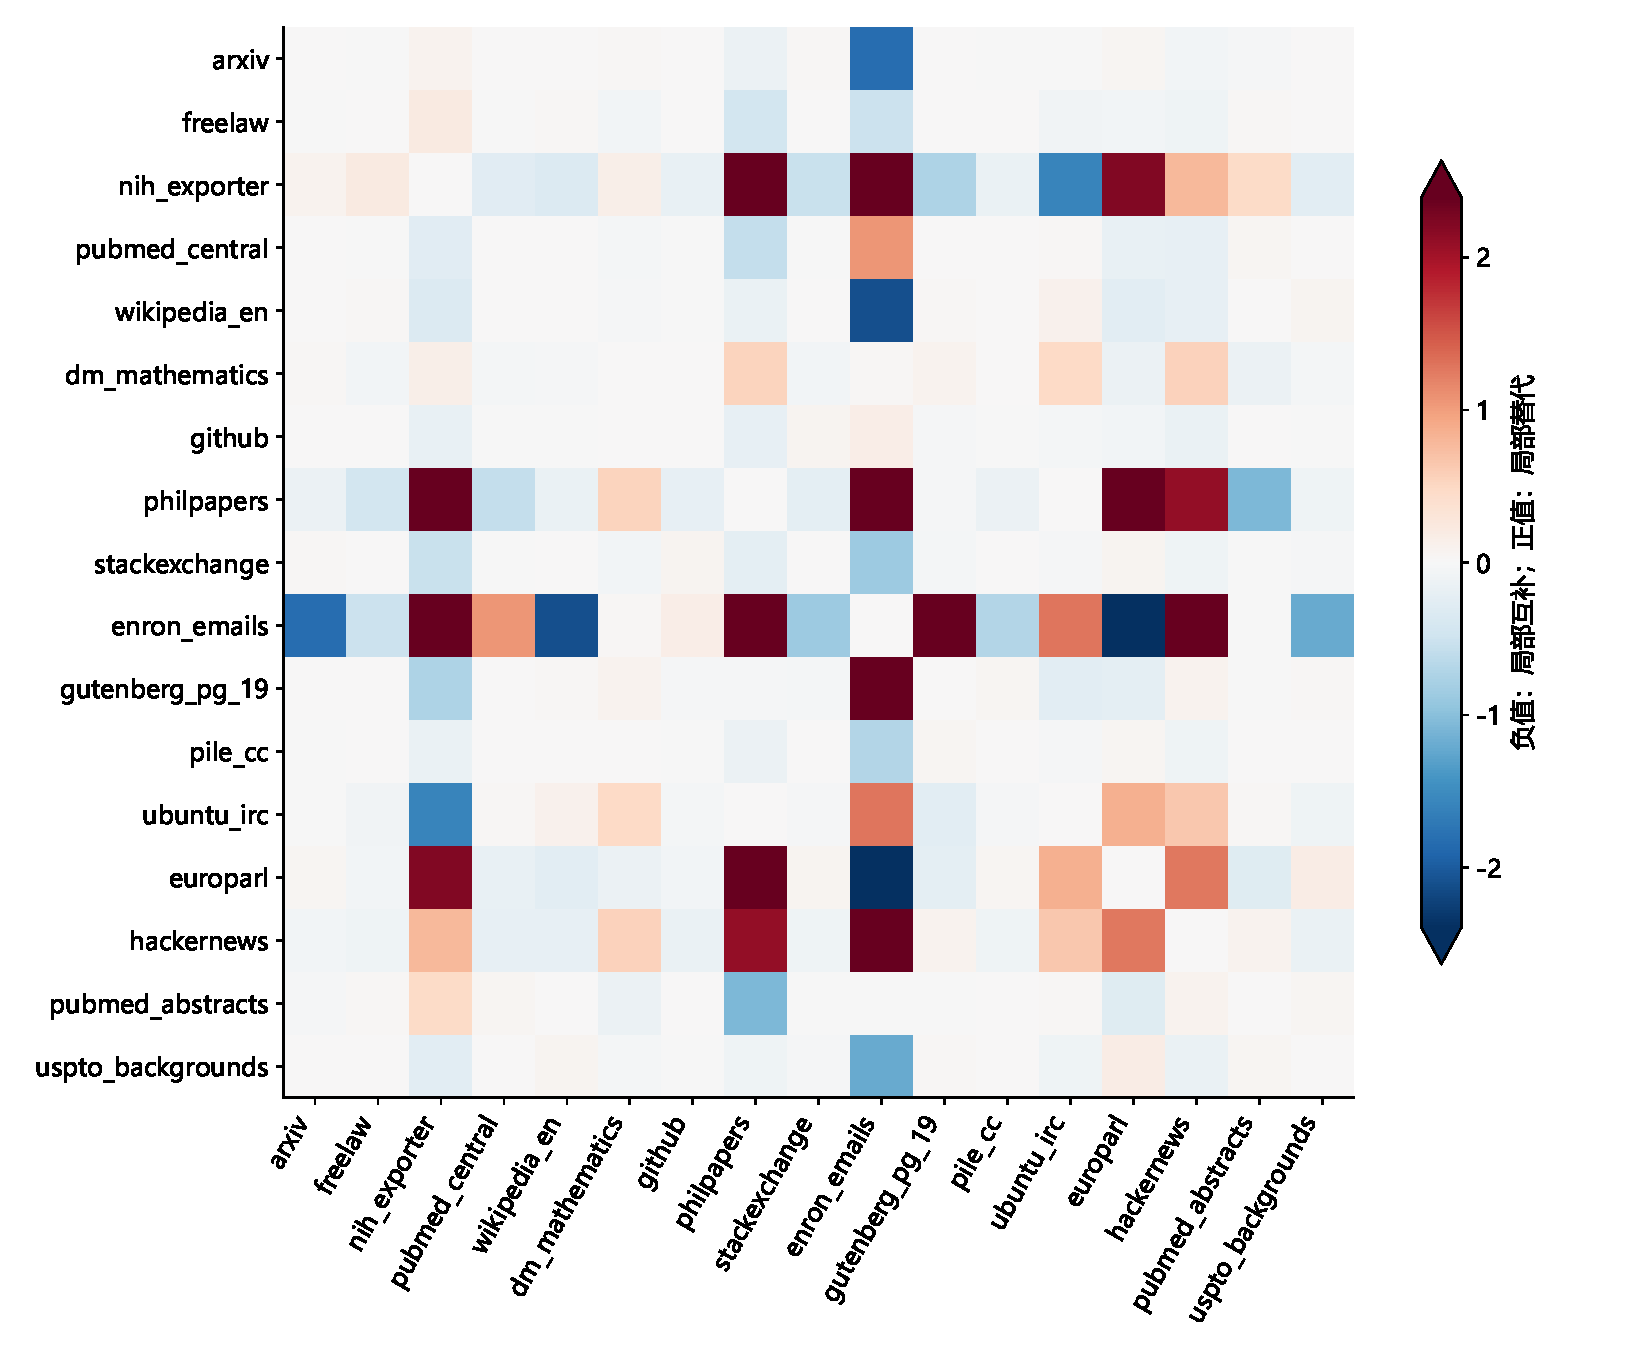
\includegraphics[width=\linewidth]{figures/q2_fig04_domain_interactions.pdf}
         \caption{常规质量路径下的领域局部交互}
         \label{fig:p2_interaction}
        \end{figure}
        
        \subsubsection{质量尺度与配比迁移的敏感性}  % 5.3.7
        质量量尺换算是资源替代结论的重要不确定性。保持式\eqref{eq:p2_example}的其他条件，将 $\kappa$ 分别取为 0.5、1 和 2，得到表\ref{tab:p2_sensitivity}。等效扩容比例由 15.66\% 变为 83.97\%，变化幅度明显大于固定模型下的 Bootstrap 区间。因此，34.35\% 应解释为主情景估计，而不是不依赖质量定义的固定比例。
        
        \begin{table}[H]
         \centering
         \caption{质量量尺对等效扩容结果的影响}
         \label{tab:p2_sensitivity}
         \begin{tabular}{ccc}
          \toprule
          质量尺度 $\kappa$ & 等效参数量 / B & 相对原 7B 的扩容比例 \\
          \midrule
          0.5 & 8.095896 & 15.66\% \\
          1.0 & 9.404464 & 34.35\% \\
          2.0 & 12.877917 & 83.97\% \\
          \bottomrule
         \end{tabular}
        \end{table}
        
        对配比迁移，比较各配方的 13 域平均损失排序，在 1M、60M、1B 检验集上的 Spearman 相关系数分别为 0.689、0.660 和 0.492；在估算的 10B、70B 配方表中则分别为 $-0.599$ 和 $-0.675$，尚不支持大规模下保持相同排序的结论。这里评价的是 13 个验证领域平均 Loss 的排序，与问题一逐验证域计算相关系数再取平均的指标不同。此外，沿常规质量路径，任意正 $\lambda_p$ 都保留同样的配方排序，故排序成绩不能用于唯一确定迁移幅度。

        \subsubsection{大模型外推的适用边界}  % 5.3.8
        B1 支持的参数量范围约为 0.070542B 至 11.965825B，数据量范围为 0.134B 至 299.893B tokens。B9、B10 所涉及的大模型在质量与配比缺失时，采用参考条件进行情景计算，其结果不作为实测精度结论。本文给出的广义标度律能够在明确假设下统一计算规模、质量和配比的作用，并为后续资源配置提供边际收益与替代条件；其跨来源强度及大规模适用性仍需统一验证口径下的联合训练实验进一步检验。

        \subsubsection{小结}  % 5.3.9
        本问将问题一的配方响应与附件 B 的规模信息衔接，得到同时包含参数量、数据量、质量和领域配比的广义标度律。分阶段估计得到参数指数 $\widehat\alpha=0.339921$、数据指数 $\widehat\beta=0.279796$ 和质量响应 $\widehat\gamma=0.410160$。质量项在 B6 半合成数据的分组验证中降低预测误差，但 B8 的方向冲突表明该规律存在明确的来源边界。

        在 7B 参数、300B tokens 的主情景下，质量提高 0.1 约等效于扩容至 9.404B；这一结果受质量量尺假设影响，不能直接转换为固定的经济收益。领域边际和交互关系仅表示参考配方邻域内的模型响应。上述估计、条件与不确定性共同构成后续资源配置分析的输入。
        
% \section{问题三}   % 6
%     \subsection{问题分析}

%     问题三要求在给定总算力下联合配置参数规模、训练数据量与数据质量。问题二已经给出三类资源共同决定验证 Loss 的广义标度律，但直接优化仍面临三个困难：其一，质量改善需要额外处理算力，且三类成本曲线的边际增长速度不同；其二，长上下文注意力会挤占基础训练预算；其三，领域配比在大规模区间的迁移强度没有被稳定识别。为保持证据边界，本文把参考配比作为主情景，只将前两问已经评价过的经验配方作为离散敏感性候选。

%     参数量和训练数据量的联合配置沿用计算最优训练的基本思想\textsuperscript{\cite{hoffmann2022chinchilla}}。对每个算力预算、质量成本函数和上下文长度分别求解，并用活跃约束变化、资源份额突变及弹性突变识别结构性转移。这样既能给出最优配置，也能解释新增算力在不同用途之间的流向。

%     \subsection{模型建立}

%         \subsubsection{目标函数与质量响应}
%         继承问题二的广义标度律，令 $n=N/10^9$、$d=D/10^{11}$，则
%         \begin{equation}
%         L(N,D,Q,\bm p)=E+\left(An^{-\alpha}+Bd^{-\beta}\right)
%         \exp\left\{\gamma\kappa[\bar Q(\bm p)-Q]+\lambda_p h(\bm p)\right\}.
%         \label{eq:p3_loss}
%         \end{equation}
%         主模型固定 $\bm p=\bm p_0$，此时 $h(\bm p_0)=0$、$\bar Q(\bm p_0)=Q_0$。三类质量成本函数分别为
%         \begin{equation}
%         g_{\exp}(Q)=10^7e^{6Q},\quad
%         g_{\mathrm{pow}}(Q)=5\times10^9Q^4,\quad
%         g_{\log}(Q)=2\times10^9\ln(1+10Q).
%         \label{eq:p3_quality_cost}
%         \end{equation}
%         令当前配比的基线质量为 $Q_b$，只对高于基线的质量提升计费：
%         \begin{equation}
%         C_{qual}=D[g_c(Q)-g_c(Q_b)]_+.
%         \label{eq:p3_quality_compute}
%         \end{equation}

%         \subsubsection{统一算力约束}
%         基础训练算力取 $C_{train}=6ND$，长上下文注意力开销采用题设代理式
%         \begin{equation}
%         C_{attn}=\eta NDL_{ctx},\qquad \eta=2\times10^{-4}.
%         \label{eq:p3_attention}
%         \end{equation}
%         因而优化问题为
%         \begin{equation}
%         \begin{aligned}
%         \min_{N,D,Q,\bm p}\quad &L(N,D,Q,\bm p),\\
%         \mathrm{s.t.}\quad &6ND+D[g_c(Q)-g_c(Q_b)]_++\eta NDL_{ctx}\le C,\\
%         &Q_b\le Q\le1,\quad N_{\min}\le N\le N_{\max},\quad
%         D_{\min}\le D\le D_{\max}.
%         \end{aligned}
%         \label{eq:p3_optimization}
%         \end{equation}
%         由于式\eqref{eq:p3_loss}随 $D$ 单调下降，非退化最优解使用全部预算，可将数据量解析消去：
%         \begin{equation}
%         D(N,Q)=\frac{C}{(6+\eta L_{ctx})N+[g_c(Q)-g_c(Q_b)]_+}.
%         \label{eq:p3_eliminate_d}
%         \end{equation}
%         原三维连续问题遂转化为 $(\log N,Q)$ 上的二维有界优化。代码先在对数网格上搜索，再调用 SLSQP 从优良初值细化\textsuperscript{\cite{virtanen2020scipy}}；候选配比策略则在外层枚举 48 个保留配方。该过程降低初值敏感性，但不构成连续单纯形上的全局最优证明。

%         \subsubsection{长上下文临界点与结构转移}
%         注意力开销和基础训练开销之比为
%         \begin{equation}
%         \frac{C_{attn}}{C_{train}}=\frac{\eta L_{ctx}}6.
%         \label{eq:p3_attention_ratio}
%         \end{equation}
%         二者相等时 $L_{ctx}^{crit}=6/\eta=30000$。C7 给出的 2048、4096、8192 位于临界点以下，32768 与 131072 位于临界点以上。本文把质量状态改变、经验配方切换、相邻预算资源份额总变差超过 0.10 或 $N,D$ 弹性变化超过 0.35 记为结构性转移；由于预算采用离散网格，转移只报告区间。

%     \subsection{建模结果}

%         表\ref{tab:p3_allocations}给出固定参考配比、$L_{ctx}=8192$ 时的代表性配置。低预算下，三类成本函数对质量投入的选择差异明显：指数型得到内点质量 $Q=0.7960$，幂函数型保持基线质量，对数渐进型则直接达到质量上界。预算提高到 $10^{22}$ FLOPs 后三种情景均达到 $Q=1$，新增预算主要流向参数量和训练数据量。

%         \begin{table}[H]
%         \centering
%         \small
%         \caption{固定参考配比和 $L_{ctx}=8192$ 下的最优资源配置}
%         \label{tab:p3_allocations}
%         \begin{tabular}{lrrrrr}
%         \toprule
%         成本函数 & $C$/FLOPs & $N$/B & $D$/B tokens & $Q^*$ & 预测 Loss \\
%         \midrule
%         指数型 & $10^{19}$ & 0.292 & 3.309 & 0.7960 & 3.0112 \\
%         指数型 & $10^{22}$ & 5.127 & 233.604 & 1.0000 & 2.0926 \\
%         指数型 & $10^{24}$ & 37.527 & 3444.850 & 1.0000 & 1.8858 \\
%         幂函数型 & $10^{19}$ & 0.204 & 6.404 & 0.6109 & 3.0347 \\
%         幂函数型 & $10^{22}$ & 5.210 & 226.770 & 1.0000 & 2.0936 \\
%         幂函数型 & $10^{24}$ & 37.624 & 3428.260 & 1.0000 & 1.8859 \\
%         对数渐进型 & $10^{19}$ & 0.298 & 3.175 & 1.0000 & 2.9105 \\
%         对数渐进型 & $10^{22}$ & 4.753 & 268.966 & 1.0000 & 2.0882 \\
%         对数渐进型 & $10^{24}$ & 37.112 & 3516.766 & 1.0000 & 1.8855 \\
%         \bottomrule
%         \end{tabular}
%         \end{table}

%         \begin{figure}[H]
%         \centering
%         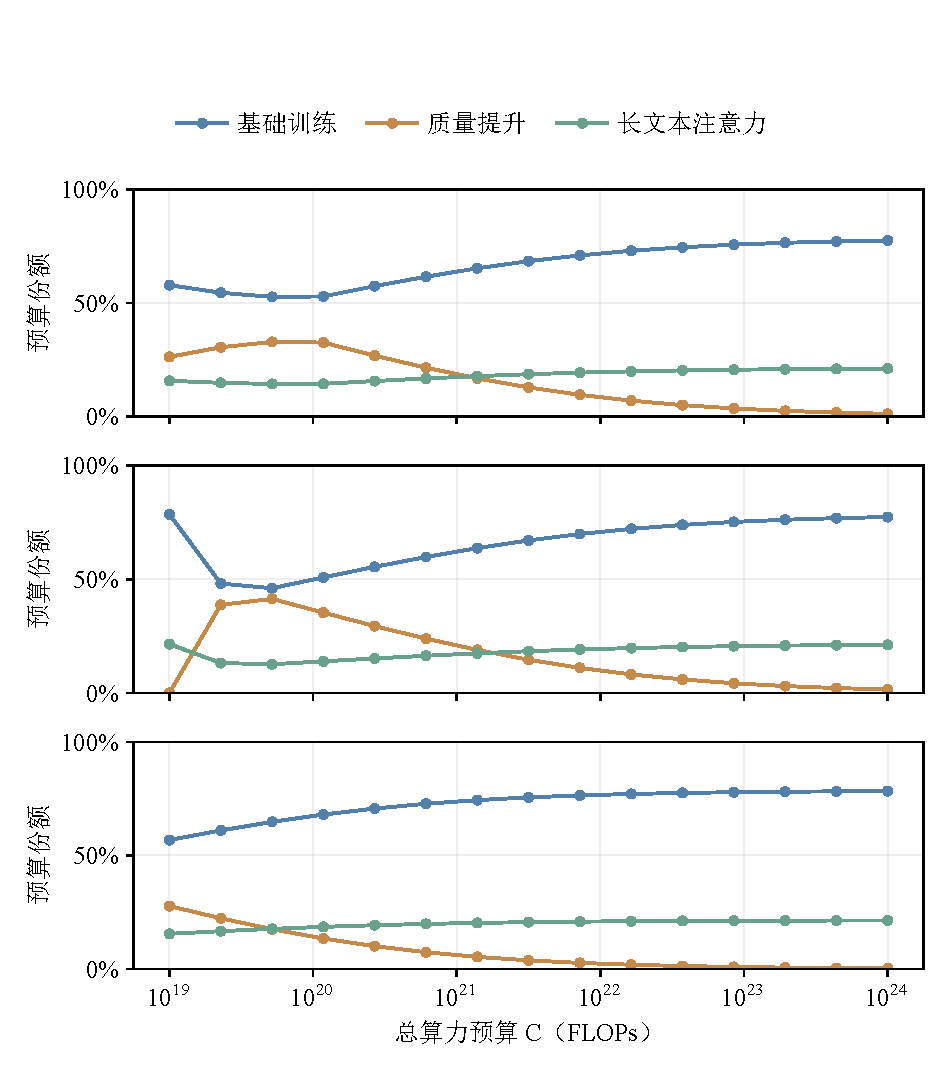
\includegraphics[width=\linewidth]{figures/q3_fig01_resource_allocation_shares.pdf}
%         \caption{三类质量成本函数下的资源份额路径}
%         \label{fig:p3_shares}
%         \end{figure}

%         图\ref{fig:p3_shares}显示，质量达到上界后，其预算份额随总预算增加而下降；基础训练重新成为主要开销。图\ref{fig:p3_paths}进一步表明 $N$ 与 $D$ 随预算近似按幂律增长，而 $Q$ 呈现“基线、内点、上界”的活跃状态切换。15 点预算网格共识别出 44 个候选转移区间，这些区间用于提示资源策略变化，不应解释为无误差的精确阈值。

%         \begin{figure}[H]
%         \centering
%         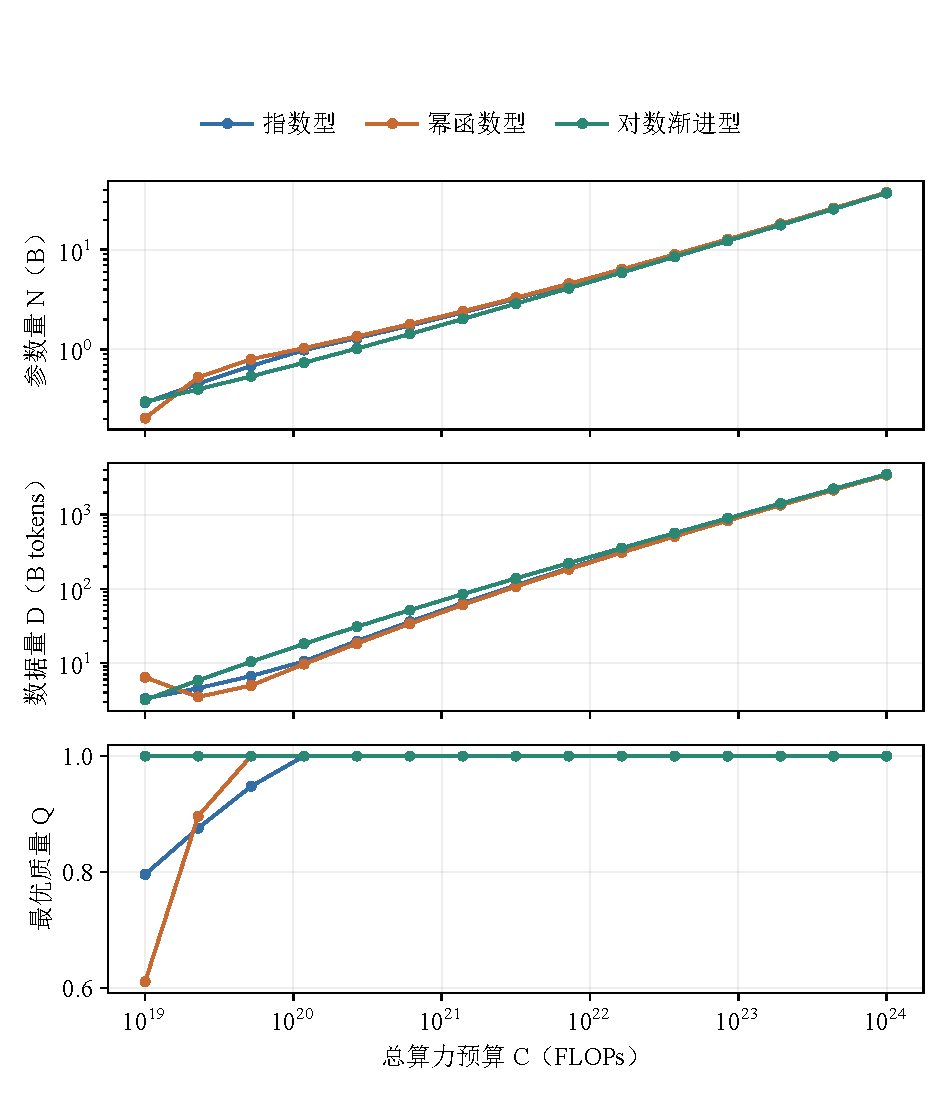
\includegraphics[width=\linewidth]{figures/q3_fig02_optimal_N_D_Q_paths.pdf}
%         \caption{最优参数量、训练数据量与质量随预算的变化}
%         \label{fig:p3_paths}
%         \end{figure}

%         上下文长度敏感性见图\ref{fig:p3_context}。以指数型成本和 $C=10^{22}$ FLOPs 为例，$L_{ctx}$ 从 2048 增至 131072 时，预测 Loss 从 2.0824 上升至 2.1884；超过临界长度 30000 后，注意力开销成为主要预算项，压缩了可用于参数量和训练数据量的算力。

%         \begin{figure}[H]
%         \centering
%         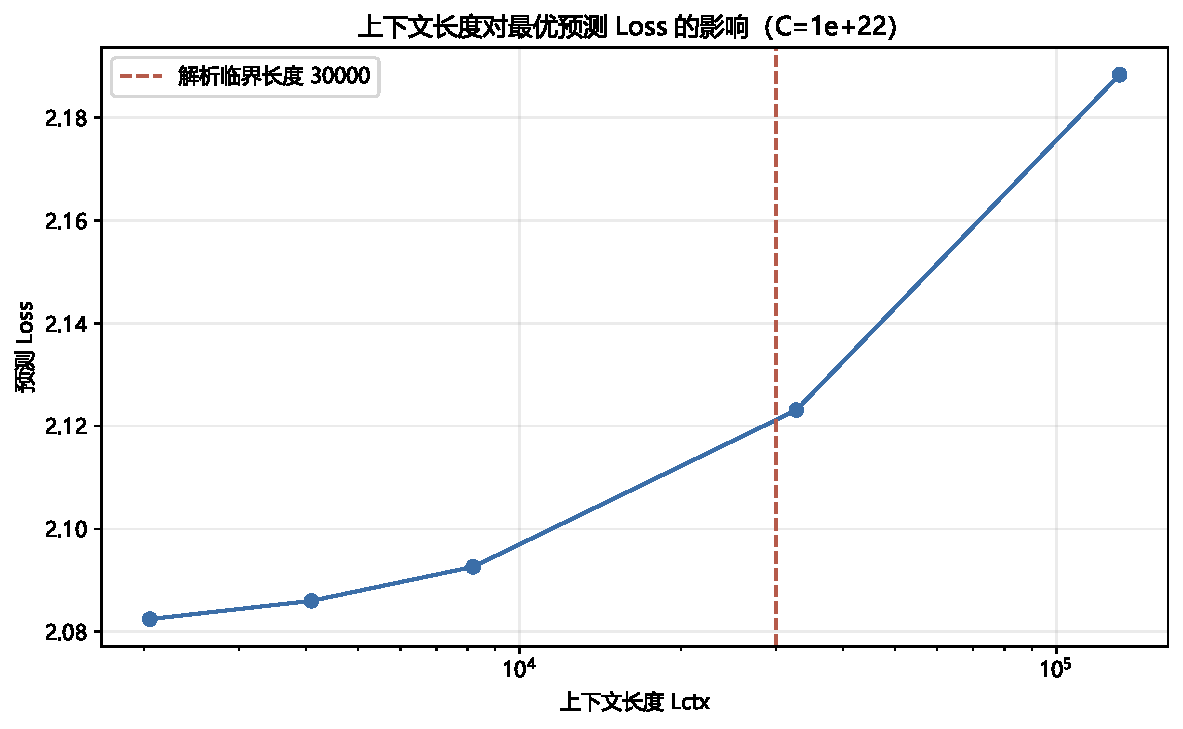
\includegraphics[width=0.82\linewidth]{figures/q3_fig03_context_length_sensitivity.pdf}
%         \caption{上下文长度对最优预测 Loss 的影响}
%         \label{fig:p3_context}
%         \end{figure}

%         在 $L_{ctx}=8192$ 的配比敏感性中，经验候选配方可进一步降低条件预测 Loss，但候选仅来自前两问已出现的配方，且大模型尺度上的配比迁移并不稳定。因此本文把固定参考配比作为主结论；$10^{24}$ FLOPs 下的 $N,D$ 已超出 B1 支持范围，相关结果仅作条件外推。

\section{问题三}

    \subsection{问题分析}

    问题三要求在给定总算力下联合配置参数规模、训练数据量与数据质量。问题二已经给出三类资源共同决定验证 Loss 的广义标度律，但直接优化仍面临三个困难：其一，质量改善需要额外处理算力，且三类成本曲线的边际增长速度不同；其二，长上下文注意力会挤占基础训练预算；其三，领域配比在大规模区间的迁移强度没有被稳定识别。为保持证据边界，本文把参考配比作为主情景，只将前两问已经评价过的经验配方作为离散敏感性候选。

    参数量和训练数据量的联合配置沿用计算最优训练的基本思想\textsuperscript{\cite{hoffmann2022chinchilla}}。本文区分两组实验：一组改变总算力预算，考察最优配置与资源投入的结构性转移；另一组固定总预算，比较上下文长度、质量成本机制和候选配比的影响。对每个情景分别求解，并用活跃约束变化、资源份额变化及预算弹性变化识别候选转移区间，从而解释新增算力在不同用途之间的分配。

    \subsection{模型建立}

        \subsubsection{目标函数与质量响应}

        继承问题二的广义标度律，令 $n=N/10^9$、$d=D/10^{11}$，则
        \begin{equation}
        L(N,D,Q,\bm p)
        =E+\left(An^{-\alpha}+Bd^{-\beta}\right)
        \exp\left\{\gamma\kappa[\bar Q(\bm p)-Q]+\lambda_p h(\bm p)\right\}.
        \label{eq:p3_loss}
        \end{equation}

        其中，$\bar Q(\bm p)$ 表示配比 $\bm p$ 的基线质量，$h(\bm p)$ 表示沿用问题二的相对配比响应。主情景固定 $\bm p=\bm p_0$，此时 $h(\bm p_0)=0$，$\bar Q(\bm p_0)=Q_0=0.6109137$。当前计算取 $\kappa=\lambda_p=1$，作为沿用问题二的情景设定；其中配比迁移强度并非由现有数据独立识别。

        三类质量成本函数分别为
        \begin{equation}
        \begin{aligned}
        g_{\exp}(Q)&=10^7e^{6Q},\\
        g_{\mathrm{pow}}(Q)&=5\times10^9Q^4,\\
        g_{\log}(Q)&=2\times10^9\ln(1+10Q).
        \end{aligned}
        \label{eq:p3_quality_cost}
        \end{equation}

        对任意配比，定义 $Q_b=\bar Q(\bm p)$，只对高于该基线的质量提升计费：
        \begin{equation}
        C_{qual}=D[g_c(Q)-g_c(Q_b)]_+,
        \qquad [x]_+=\max(x,0).
        \label{eq:p3_quality_compute}
        \end{equation}
        因此，参考策略和候选策略均从各自的基线质量开始计费。配比改变时，三类 $g_c$ 的函数形式及参数保持不变，但基线质量和最优资源配置可以变化。

        \subsubsection{统一算力约束与降维求解}

        基础训练算力取 $C_{train}=6ND$，长上下文注意力开销采用题设代理式
        \begin{equation}
        C_{attn}=\eta NDL_{ctx},
        \qquad \eta=2\times10^{-4}.
        \label{eq:p3_attention}
        \end{equation}

        主情景取配比集合 $\mathcal P=\{\bm p_0\}$，候选敏感性分析取 $\mathcal P=\mathcal P_{\mathrm{emp}}$，其中 $\mathcal P_{\mathrm{emp}}$ 为保留的经验配方集合。优化问题为
        \begin{equation}
        \begin{aligned}
        \min_{N,D,Q,\bm p}\quad &L(N,D,Q,\bm p),\\
        \mathrm{s.t.}\quad
        &6ND+D[g_c(Q)-g_c(Q_b)]_++\eta NDL_{ctx}\le C,\\
        &Q_b=\bar Q(\bm p),\quad Q_b\le Q\le1,\\
        &N_{\min}\le N\le N_{\max},\\
        &D_{\min}\le D\le D_{\max},\\
        &\bm p\in\mathcal P.
        \end{aligned}
        \label{eq:p3_optimization}
        \end{equation}

        本模型未另行计入改变配比所需的独立采购、采样等开销；配比通过基线质量和 Loss 响应影响资源配置。

        在数据量上界未活跃时，由于式\eqref{eq:p3_loss}随 $D$ 单调下降，最优解的预算约束取等号。本次数值结果满足这一条件，因此可将数据量解析消去：
        \begin{equation}
        D(N,Q)=\frac{C}{(6+\eta L_{ctx})N+[g_c(Q)-g_c(Q_b)]_+}.
        \label{eq:p3_eliminate_d}
        \end{equation}
        消元后仍保留约束 $D_{\min}\le D(N,Q)\le D_{\max}$。对每个固定配比，连续优化问题转化为 $(\log_{10}N,Q)$ 上的二维有界优化。

        求解时先进行粗网格搜索，再调用 SLSQP 从网格得到的优良初值细化\textsuperscript{\cite{virtanen2020scipy}}。候选策略先比较全部 48 条保留记录的粗网格结果，再对排名前三的候选进行连续优化。此外，在固定预算 $C_0=10^{22}$ FLOPs、$L_{ctx}=8192$ 的候选对照中，对全部保留候选逐一细化，所得最佳 Loss 与原候选策略一致。该核对仅针对指定对照情景，不构成所有预算情景或连续配比单纯形上的全局最优证明。

        \subsubsection{长上下文临界点与结构转移}

        注意力开销和基础训练开销之比为
        \begin{equation}
        \frac{C_{attn}}{C_{train}}=\frac{\eta L_{ctx}}{6}.
        \label{eq:p3_attention_ratio}
        \end{equation}
        二者相等时，$L_{ctx}^{crit}=6/\eta=30000$。C7 给出的 2048、4096、8192 位于临界点以下，32768 与 131072 位于临界点以上。该临界点仅表示注意力开销等于基础训练开销，不表示注意力占总预算的 $50\%$，也不是预测 Loss 的跳变点。

        令相邻预算为 $C_i,C_{i+1}$，三项成本份额组成向量 $\bm s_i=(s_{train,i},s_{qual,i},s_{attn,i})$。资源份额总变差与预算弹性分别定义为
        \begin{equation}
        \begin{aligned}
        \mathrm{TV}_i
        &=\frac12\sum_{k\in\{train,qual,attn\}}|s_{k,i+1}-s_{k,i}|,\\
        \varepsilon_{X,i}
        &=\frac{\ln(X_{i+1}/X_i)}{\ln(C_{i+1}/C_i)},
        \qquad X\in\{N,D\}.
        \end{aligned}
        \label{eq:p3_transition_indicators}
        \end{equation}

        当质量活跃状态改变、候选配方切换、$\mathrm{TV}_i\ge0.10$，或相邻区间的 $N,D$ 弹性变化最大值达到 $0.35$ 时，将对应预算区间记为候选结构性转移区间。这些阈值用于数值诊断；由于预算采用离散网格，本文只报告转移区间，不将其解释为精确临界预算。

        \subsubsection{实验设置与固定预算对照}

        本文区分预算路径分析和固定预算对照。预算路径在 $10^{19}$ 至 $10^{24}$ FLOPs 之间设置 15 个对数等距点，并在 $10^{19}$、$10^{22}$、$10^{24}$ FLOPs 三档代表性预算下报告资源配置。

        上下文敏感性分析单独固定总预算 $C_0=10^{22}$ FLOPs，比较三类质量成本函数和 C7 的五种上下文长度。所有对照沿用相同的标度律参数、注意力系数和成本函数参数，并在每个情景下重新优化 $N,D,Q$，使基础训练、质量处理和注意力开销之和等于 $C_0$。固定参考配比构成主结果；候选策略在相同预算、上下文和成本机制下进行配对比较。

        对上下文敏感性，定义相对最短上下文的变化为
        \begin{equation}
        \Delta L_{\mathrm{ctx},c}(\ell)
        =L_c^*(C_0,\ell)-L_c^*(C_0,2048).
        \label{eq:p3_context_loss_change}
        \end{equation}
        当前目标函数未包含上下文长度对 Loss 的直接收益项，因而该指标仅反映固定预算下的注意力开销增加及资源再配置效应，不能用于判断实际长文本能力的变化。

    \subsection{建模结果}

        \subsubsection{不同预算下的最优资源配置}

        表\ref{tab:p3_allocations}给出固定参考配比、$L_{ctx}=8192$ 时的代表性配置。低预算下，三类成本函数对质量投入的选择差异明显：指数型得到内点质量 $Q=0.7960$，幂函数型保持基线质量，对数渐进型则直接达到质量上界。预算提高到 $10^{22}$ FLOPs 后，三种情景均达到 $Q=1$，新增预算主要流向参数量和训练数据量。

        \begin{table}[htbp]
        \centering
        \small
        \caption{固定参考配比和 $L_{ctx}=8192$ 下的最优资源配置}
        \label{tab:p3_allocations}
        \begin{tabular}{lrrrrr}
        \toprule
        成本函数 & $C$/FLOPs & $N$/B & $D$/B tokens & $Q^*$ & 预测 Loss \\
        \midrule
        指数型 & $10^{19}$ & 0.292 & 3.309 & 0.7960 & 3.0112 \\
        指数型 & $10^{22}$ & 5.127 & 233.604 & 1.0000 & 2.0926 \\
        指数型 & $10^{24}$ & 37.527 & 3444.850 & 1.0000 & 1.8858 \\
        幂函数型 & $10^{19}$ & 0.204 & 6.404 & 0.6109 & 3.0347 \\
        幂函数型 & $10^{22}$ & 5.210 & 226.770 & 1.0000 & 2.0936 \\
        幂函数型 & $10^{24}$ & 37.624 & 3428.260 & 1.0000 & 1.8859 \\
        对数渐进型 & $10^{19}$ & 0.298 & 3.175 & 1.0000 & 2.9105 \\
        对数渐进型 & $10^{22}$ & 4.753 & 268.966 & 1.0000 & 2.0882 \\
        对数渐进型 & $10^{24}$ & 37.112 & 3516.766 & 1.0000 & 1.8855 \\
        \bottomrule
        \end{tabular}
        \end{table}

        \begin{figure}[htbp]
        \centering
        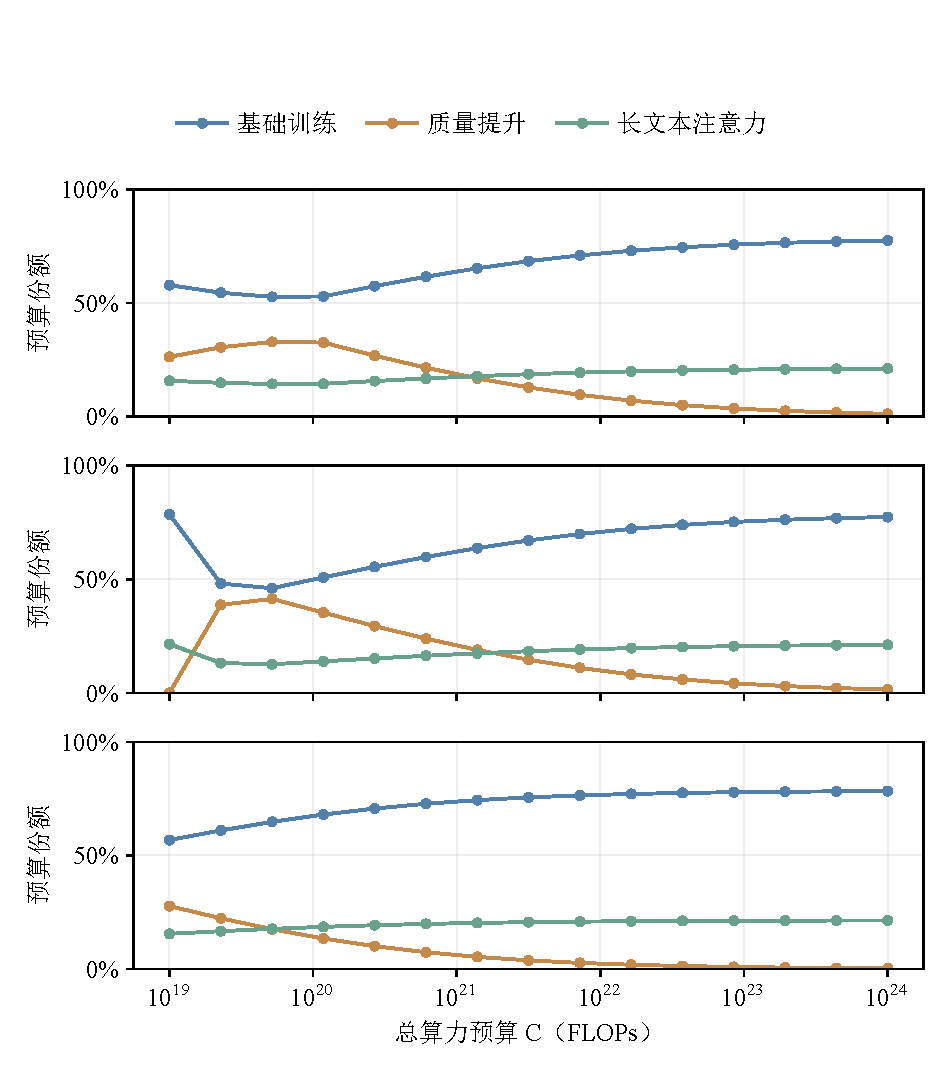
\includegraphics[width=\linewidth]{figures/q3_fig01_resource_allocation_shares.pdf}
        \caption{固定参考配比下的资源份额路径（$L_{ctx}=8192$ ）}
        \label{fig:p3_shares}
        \end{figure}

        图\ref{fig:p3_shares}显示，当质量达到上界后，质量处理的预算份额随总预算增加而下降，基础训练成为主要开销。图\ref{fig:p3_paths}进一步表明，$N$ 与 $D$ 随预算近似按幂律增长，不同成本机制下的质量选择表现出基线、内点和上界等活跃状态，但并非每条路径都依次经历全部状态。

        在两种配比策略、三类成本模型和五种上下文组成的 30 条预算路径中，15 点预算网格共得到 44 条候选转移记录，其中参考策略 16 条、候选策略 28 条。图\ref{fig:p3_shares}和图\ref{fig:p3_paths}对应的固定参考配比、$L_{ctx}=8192$ 情景合计包含 4 条。不同情景的记录可能落在相同预算区间，因此这些记录不代表 44 个互不相同的精确临界预算。

        \begin{figure}[htbp]
        \centering
        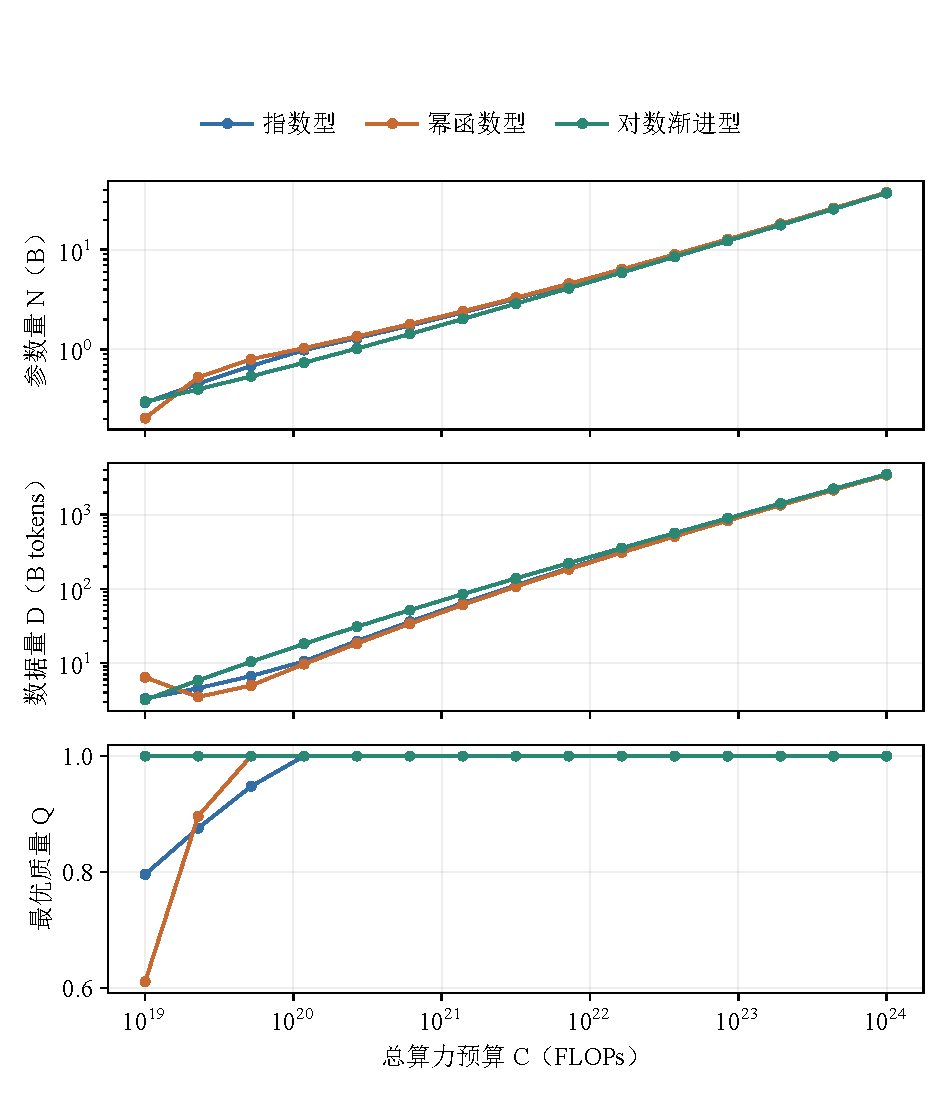
\includegraphics[width=\linewidth]{figures/q3_fig02_optimal_N_D_Q_paths.pdf}
        \caption{固定参考配比、$L_{ctx}=8192$ 时，最优参数量、训练数据量与质量随预算的变化}
        \label{fig:p3_paths}
        \end{figure}

        \subsubsection{固定总预算下的上下文与成本模型比较}

        在固定总预算 $C_0=10^{22}$ FLOPs 和参考配比下，上下文长度对预测 Loss 的影响见图\ref{fig:p3_context}。图中竖虚线表示注意力开销等于基础训练开销的长度且当前模型未计入上下文长度的直接收益。当 $L_{ctx}$ 从 2048 增至 131072 时，指数型、幂函数型和对数渐进型成本下的预测 Loss 分别由 2.08243、2.08347、2.07778 上升至 2.18838、2.18898、2.18579，对应增幅约为 $5.09\%$、$5.06\%$ 和 $5.20\%$。三类成本机制均表现出固定预算下的资源挤占效应。

        \begin{figure}[htbp]
        \centering
        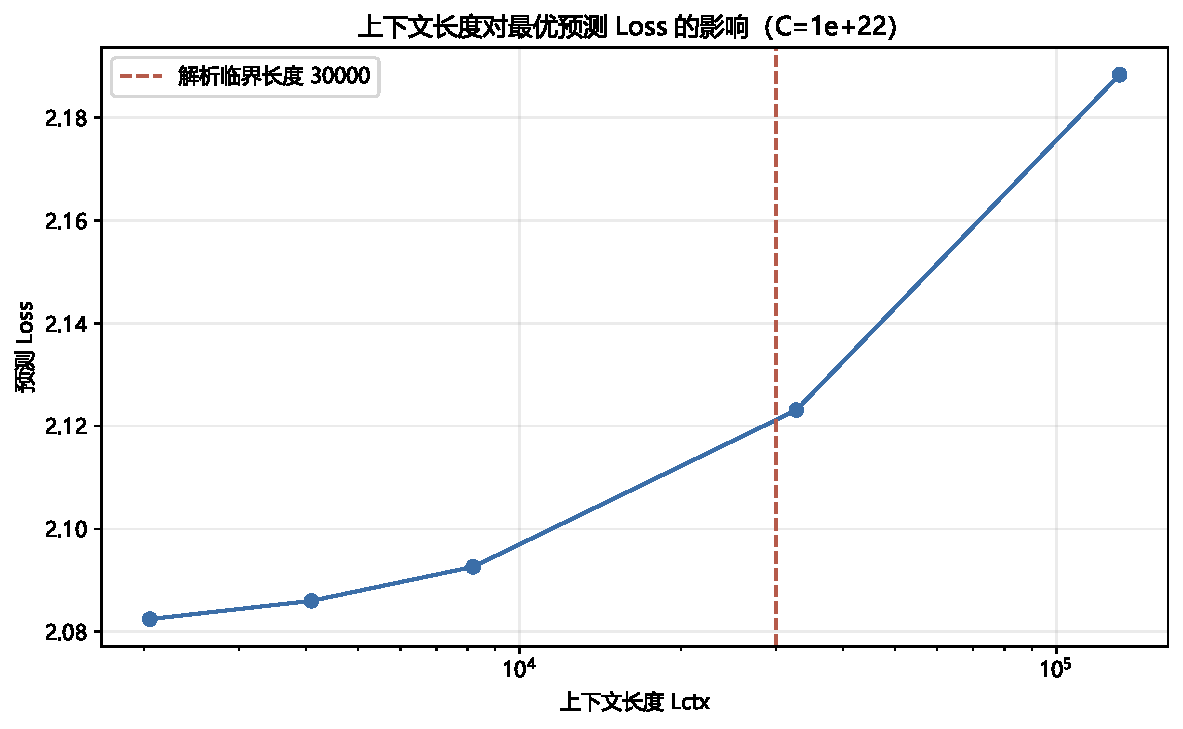
\includegraphics[width=\linewidth]{figures/q3_fig03_context_length_sensitivity.pdf}
        \caption{固定 $C_0=10^{22}$ FLOPs 和参考配比时，上下文长度对最优预测 Loss 的影响}
        \label{fig:p3_context}
        \end{figure}

        图\ref{fig:p3_context_costs}进一步展示三项成本份额的变化。从最短到最长上下文，指数型、幂函数型和对数渐进型的注意力份额分别由 $5.80\%$、$5.72\%$、$6.23\%$ 增至 $77.91\%$、$77.34\%$、$80.48\%$；质量处理份额则分别由 $9.22\%$、$10.54\%$、$2.57\%$ 降至 $4.26\%$、$4.96\%$、$1.10\%$。

        这组固定预算情景均有 $Q^*=1$。上下文增加后，最优参数量和训练数据量均下降，因而质量处理总成本随数据量减少而下降。这里发生变化的是最优配置下的实际成本，三类质量成本函数本身的参数并未随上下文改变。例如指数型在 $L_{ctx}=32768$ 时，注意力份额为 $48.68\%$，已超过基础训练份额，但仍未达到总预算的一半。

        \begin{figure}[htbp]
        \centering
        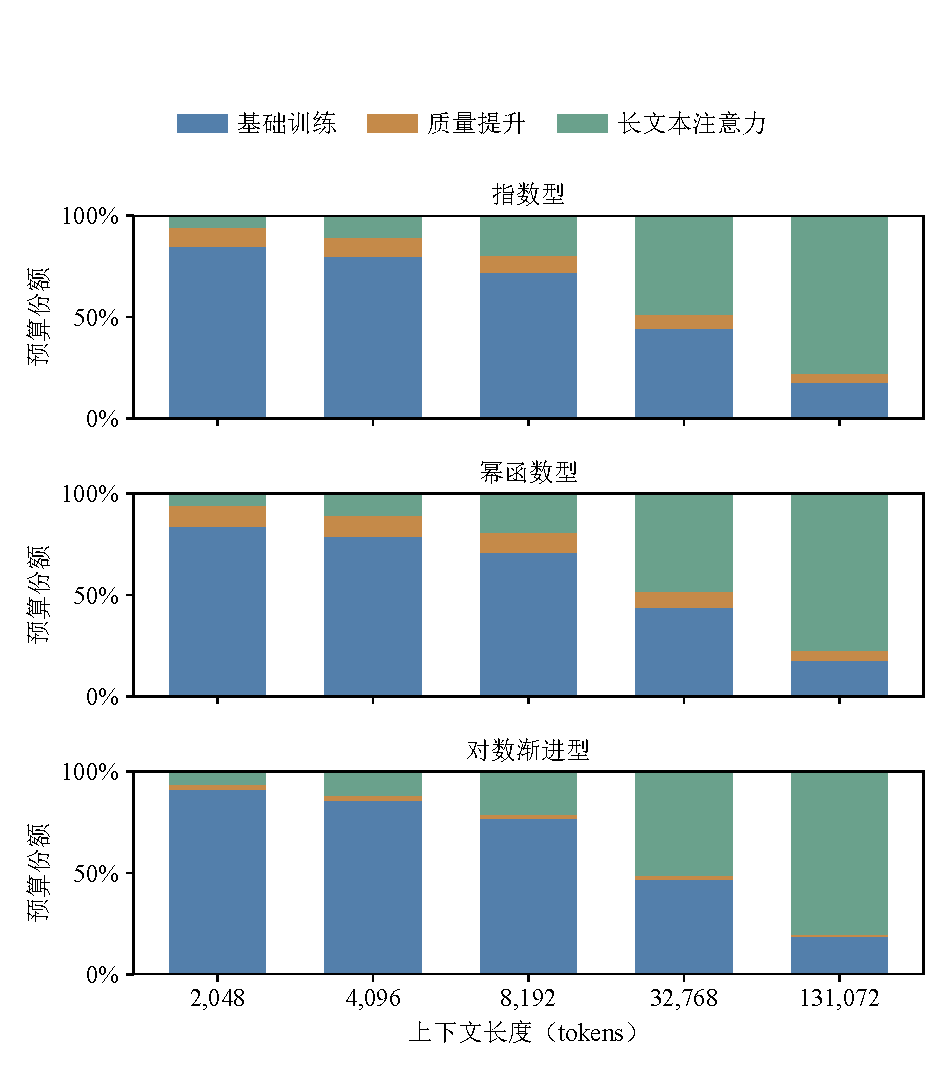
\includegraphics[width=\linewidth]{figures/q3_fig04_fixed_budget_context_costs.pdf}
        % \caption{固定 $C_0=10^{22}$ FLOPs 和参考配比时，上下文长度对基础训练、质量处理和注意力成本份额的影响。每个情景分别重新优化 $N,D,Q$，三项份额之和为 $1$。}
        \caption{固定 $C_0=10^{22}$ FLOPs 和参考配比时，上下文长度对三项成本份额的影响}
        \label{fig:p3_context_costs}
        \end{figure}

        \subsubsection{候选配比对成本与 Loss 的影响}

        在相同预算、上下文和质量成本机制下，分别求解固定参考配比与经验候选策略。定义候选策略相对于参考策略的 Loss 改善及其比例为
        \begin{equation}
        \begin{aligned}
        \Delta L_{\mathrm{mix}}
        &=L_{\mathrm{ref}}^*-L_{\mathrm{cand}}^*,\\
        R_{\mathrm{mix}}
        &=\frac{L_{\mathrm{ref}}^*-L_{\mathrm{cand}}^*}{L_{\mathrm{ref}}^*}\times100\%.
        \end{aligned}
        \label{eq:p3_mixture_improvement}
        \end{equation}
        正值表示候选策略的预测 Loss 更低。成本份额变化统一定义为候选策略减去参考策略，并以百分点报告。

        表\ref{tab:p3_mixture_comparison}给出 $C_0=10^{22}$ FLOPs、$L_{ctx}=8192$ 时的代表性结果。三类成本机制下，候选策略使预测 Loss 降低约 $2.29\%$ 至 $2.32\%$，同时质量处理成本份额略有增加。

        \begin{table}[htbp]
        \centering
        \small
        \caption{固定 $C_0=10^{22}$ FLOPs、$L_{ctx}=8192$ 时的参考与候选配比对照}
        \label{tab:p3_mixture_comparison}
        \begin{tabular}{lrrrr}
        \toprule
        成本函数 & 参考 Loss & 候选 Loss & \shortstack{Loss 降幅\\（\%）} & \shortstack{质量份额变化\\（百分点）} \\
        \midrule
        指数型 & 2.09260 & 2.04422 & 2.31 & +0.0566 \\
        幂函数型 & 2.09359 & 2.04511 & 2.32 & +0.1045 \\
        对数渐进型 & 2.08823 & 2.04038 & 2.29 & +0.0934 \\
        \bottomrule
        \end{tabular}
        \end{table}

        三类成本机制在该情景下均选中来源为 \texttt{test\_1m}、索引为 59 的候选记录，其基线质量约为 $0.5980$，低于参考配比的 $0.6109$。该配方与 \texttt{test\_60m} 中索引为 59 的记录等价。在相同目标质量下，较低的基线质量意味着更高的单位数据质量提升成本；配比响应带来的降损仍可使其最终预测 Loss 更低。因此，Loss 改善并不要求质量处理成本同步下降。

        以指数型为例，候选策略的基础训练、质量处理和注意力份额分别变化 $-0.0444$、$+0.0566$、$-0.0121$ 个百分点。未经舍入的三项变化之和为零，表明两种策略使用相同总预算，差异来自预算内部的重新分配。

        \subsubsection{结果适用范围}

        候选配比仅来自前两问已评价并保留的经验配方，其迁移强度沿用问题二的情景假设，因此上述改善属于条件预测，不能视为已经验证的大模型训练收益。本文仍以固定参考配比作为主结论。

        上下文分析仅刻画固定算力约束下的资源挤占与再配置，未识别延长上下文对任务表现的直接收益。在 $10^{24}$ FLOPs 下，表\ref{tab:p3_allocations}中的最优 $N,D$ 已超出 B1 的数据支持范围，相关结果仅用于讨论模型条件下的资源配置趋势。

% \section{问题四}   % 7
%     \subsection{问题分析}

%     前三问最终输出的是验证 Loss，而问题四使用开放模型的六项任务成绩，因此首先需要建立 Loss 到能力分数的可比桥接。历史模型的训练数据量、参数量和发布时间又存在缺失与口径差异，若直接把分数随年份的上升归因于某项技术，会混淆规模扩张、模型族构成和评测选择。本文借鉴观察型标度分析中控制规模与模型族差异的思想\textsuperscript{\cite{ruan2024observational}}，先构造参考规模 Loss，再用时间残差表示未被规模解释的共同变化。

%     分数经过 logit 变换后建模，以避免有界指标在线性外推中超过 $[0,100]$。同时，评分口径本身可能改变表观能力曲线\textsuperscript{\cite{schaeffer2023emergent}}，故 C6 桥接按可比性分层，C3 旧口径分数不与主回归直接混合。最终预测以附件截止日前三个月的 95\% 分位前沿为锚点，只解释为外生算力情景下的条件结果。

%     \subsection{模型建立}

%         \subsubsection{综合能力与参考规模项}
%         对 IFEval、BBH、MATH Lvl 5、GPQA、MUSR 和 MMLU-PRO 六项任务取等权平均：
%         \begin{equation}
%         S_i=\frac16\sum_{k=1}^{6}s_{ik},\qquad
%         z(S)=\operatorname{logit}\!\left[\operatorname{clip}(S/100,0.001,0.999)\right].
%         \label{eq:p4_score}
%         \end{equation}
%         由于历史模型通常缺少逐模型质量和配比，统一在参考条件下计算
%         \begin{equation}
%         L_i^{ref}=E+A(N_i/10^9)^{-\alpha}+B(D_i/10^{11})^{-\beta}.
%         \label{eq:p4_reference_loss}
%         \end{equation}
%         未观测的数据质量和配比差异留在残差中，不声称已经被控制。

%         \subsubsection{单调 Loss--Benchmark 桥接}
%         对任务 $k$ 建立带模型类型和模型族控制的岭回归：
%         \begin{equation}
%         z(s_{ik})=a_k-b_kL_i+c_kI_i^{chat}+\sum_{f\ne f_0}u_{kf}I_{if}+e_{ik},\qquad b_k\ge0.
%         \label{eq:p4_bridge}
%         \end{equation}
%         High 主模型只使用 7 个高可比 Pythia 样本；High+Medium 模型仅作跨族敏感性。参考综合桥接为
%         \begin{equation}
%         H(L)=\frac{100}{6}\sum_{k=1}^{6}\sigma(a_k-b_kL),\qquad G(L)=z[H(L)].
%         \label{eq:p4_bridge_function}
%         \end{equation}

%         \subsubsection{非规模时间动力学与贡献分解}
%         扣除参考规模项后定义
%         \begin{equation}
%         r_i=z(S_i)-G(L_i^{ref})
%         =a+\tau t_i+\delta I_i^{chat}+\sum_{f\ne f_0}v_fI_{if}+\varepsilon_i,
%         \label{eq:p4_dynamics}
%         \end{equation}
%         其中 $t_i$ 以附件截止日期为原点，模型族按记录数倒数加权。$\tau$ 包含未测质量、架构、对齐、污染和样本选择等共同影响，故称为非规模时间趋势。

%         令 $F(\ell,t)$ 表示固定完整样本族/类型组成时、参考 Loss 为 $\ell$、时间为 $t$ 的预测均值。对早晚组状态 $(\ell_0,t_0)$ 与 $(\ell_1,t_1)$，采用两因素 Shapley 分解：
%         \begin{equation}
%         \begin{aligned}
%         \Delta_{scale}&=\tfrac12\{F(\ell_1,t_0)-F(\ell_0,t_0)+F(\ell_1,t_1)-F(\ell_0,t_1)\},\\
%         \Delta_{time}&=\tfrac12\{F(\ell_0,t_1)-F(\ell_0,t_0)+F(\ell_1,t_1)-F(\ell_1,t_0)\}.
%         \end{aligned}
%         \label{eq:p4_shapley}
%         \end{equation}
%         两者之和严格等于模型反事实总变化，且消除了人为规定先改变规模还是先改变时间的顺序依赖。

%         \subsubsection{算力情景与能力前沿预测}
%         取截止日前一年开放语言模型训练 FLOPs 的 95\% 分位为 $C_0$，设
%         \begin{equation}
%         C(h;g)=C_0(1+g)^{h/12},\qquad g\in\{0,0.10,0.25\},\quad h\in\{12,24\}.
%         \label{eq:p4_compute_path}
%         \end{equation}
%         将各预算输入问题三求解器得到最优 Loss $L^*(C)$。以近期第 $b$ 类模型能力前沿 $F_{b,0}$ 为锚点，预测
%         \begin{equation}
%         \widehat F_b(h)=100\sigma\!\left[z(F_{b,0})+G(L^*(C(h)))-G(L^*(C_0))
%         +\rho\widehat\tau h/12\right],\quad \rho\in\{0,0.5,1\}.
%         \label{eq:p4_forecast}
%         \end{equation}
%         其中 $\rho$ 表示非规模趋势停止、保留一半或完全延续。采用 200 次分层 Bootstrap 传播桥接、模型族、前沿锚点和问题二参数的不确定性\textsuperscript{\cite{efron1979bootstrap}}。

%         \subsubsection{逐任务聚合分析}
%         定义 $\mathcal K_i$ 为 模型 \(i\) 对应于 C8 的 BBH 子任务集合，\(a_{ik}\) 为模型 \(i\) 在第 \(k\) 个 BBH 子任务上的正确率，范围为 \(0\sim1\)，\(n_{ik}\) 为第 \(k\) 个子任务的有效样本数，定义任务宏平均和任务微（加权）平均：
%         \begin{equation}    
%         B_i^{macro}=\frac{100}{|\mathcal K_i|}\sum_{k\in\mathcal K_i}a_{ik},\qquad
%         B_i^{micro}=100\frac{\sum_k n_{ik}a_{ik}}{\sum_k n_{ik}}.
%         \label{eq:p4_aggregation}
%         \end{equation}

%     \subsection{建模结果}

%         截止 2025 年 3 月 13 日，开放筛选后得到 1329 个 C1 模型，其中 52 个具有可用于参考规模项的完整密集模型记录；C6 High 桥接样本为 7 个。图\ref{fig:p4_bridge}给出分层桥接。High 留一 MAE 为 0.3335 分，略低于均值基线的 0.3756 分；跨族敏感性桥接 MAE 为 10.8775 分，高于均值基线的 10.3411 分，说明跨族映射仍不稳定。

%         \begin{figure}[H]
%         \centering
%         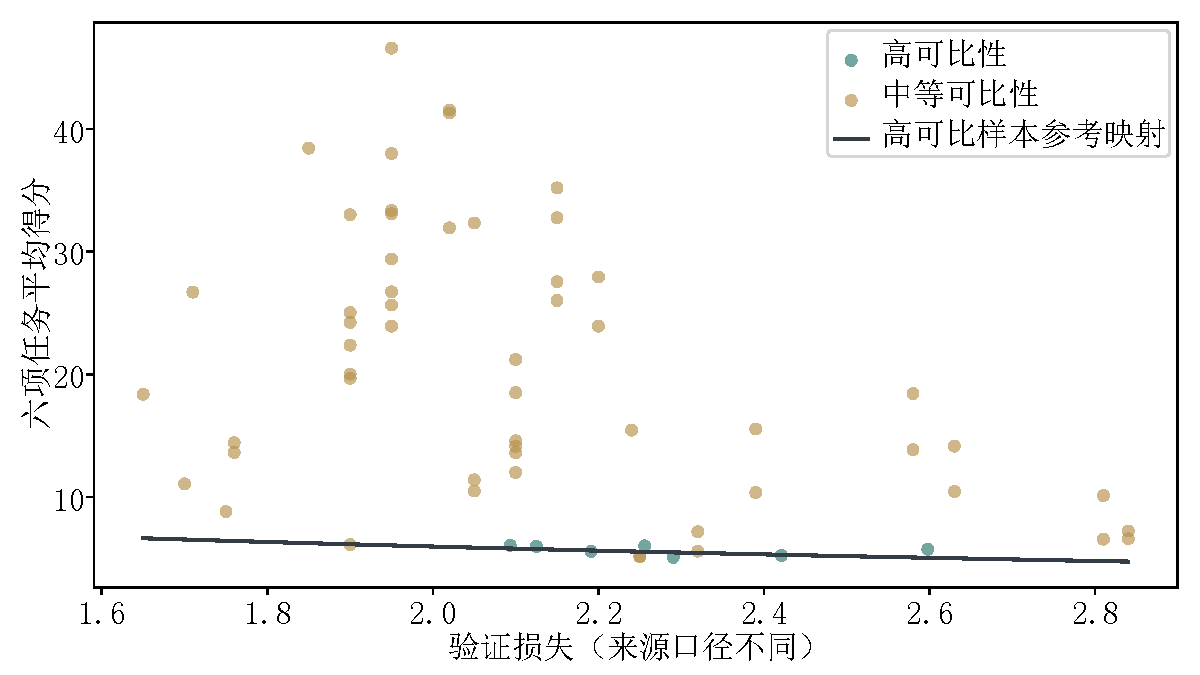
\includegraphics[width=0.86\linewidth]{figures/q4_fig01_loss_benchmark_bridge.pdf}
%         \caption{分层 Loss--Benchmark 桥接及高可比参考映射}
%         \label{fig:p4_bridge}
%         \end{figure}

%         \begin{table}[H]
%         \centering
%         \caption{问题四桥接与时间留出检验}
%         \label{tab:p4_validation}
%         \begin{tabular}{lrrr}
%         \toprule
%         检验 & 样本量 & MAE & 均值基线 MAE \\
%         \midrule
%         High 按模型留一 & 7 & 0.3335 & 0.3756 \\
%         High+Medium 按族留一 & 62 & 10.8775 & 10.3411 \\
%         60\% 时间截断 & 21 & 11.1606 & 11.1585 \\
%         75\% 时间截断 & 11 & 12.6152 & 12.7228 \\
%         85\% 时间截断 & 8 & 14.3541 & 14.1148 \\
%         \bottomrule
%         \end{tabular}
%         \end{table}

%         图\ref{fig:p4_history}展示每月新增提交模型的 95\% 分位，而非历史累计最高值，因此曲线允许下降。三个时间留出误差也未稳定优于均值基线，说明预测应理解为结构化情景而非高精度长期预测器。

%         \begin{figure}[H]
%         \centering
%         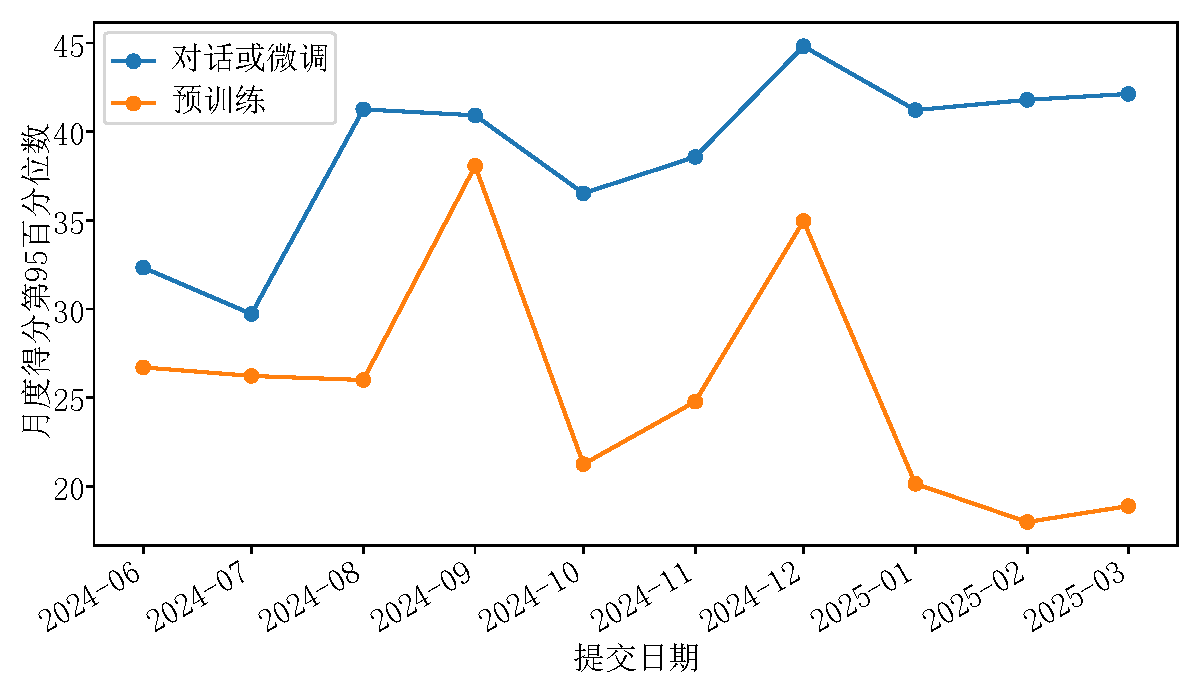
\includegraphics[width=0.88\linewidth]{figures/q4_fig02_historical_frontier.pdf}
%         \caption{开放模型六任务综合能力的月度操作性前沿}
%         \label{fig:p4_history}
%         \end{figure}

%         条件 Shapley 点估计给出总变化 3.7429 分，其中规模项 0.3380 分、非规模时间项 3.4048 分，占比分别为 9.03\% 和 90.97\%。规模项的 Bootstrap 95\% 区间为 $[-0.1420,0.6848]$ 分，对应占比区间约为 $[-2.80\%,36.83\%]$；因此不能把 90.97\% 写成已经识别的技术因果贡献。

%         % 在指数型质量成本、$L_{ctx}=8192$、非规模趋势保留一半的示例中，年算力增长 10\% 时，聊天/微调模型前沿在 12 个月和 24 个月分别为 44.26 和 46.65 分，预训练模型分别为 29.62 和 31.67 分。图\ref{fig:p4_forecast}显示三种算力增速的曲线接近，原因是 High 桥接在外推区间对 Loss 变化的分数响应较弱，并非遗漏了算力情景。

%         % \begin{figure}[H]
%         % \centering
%         % 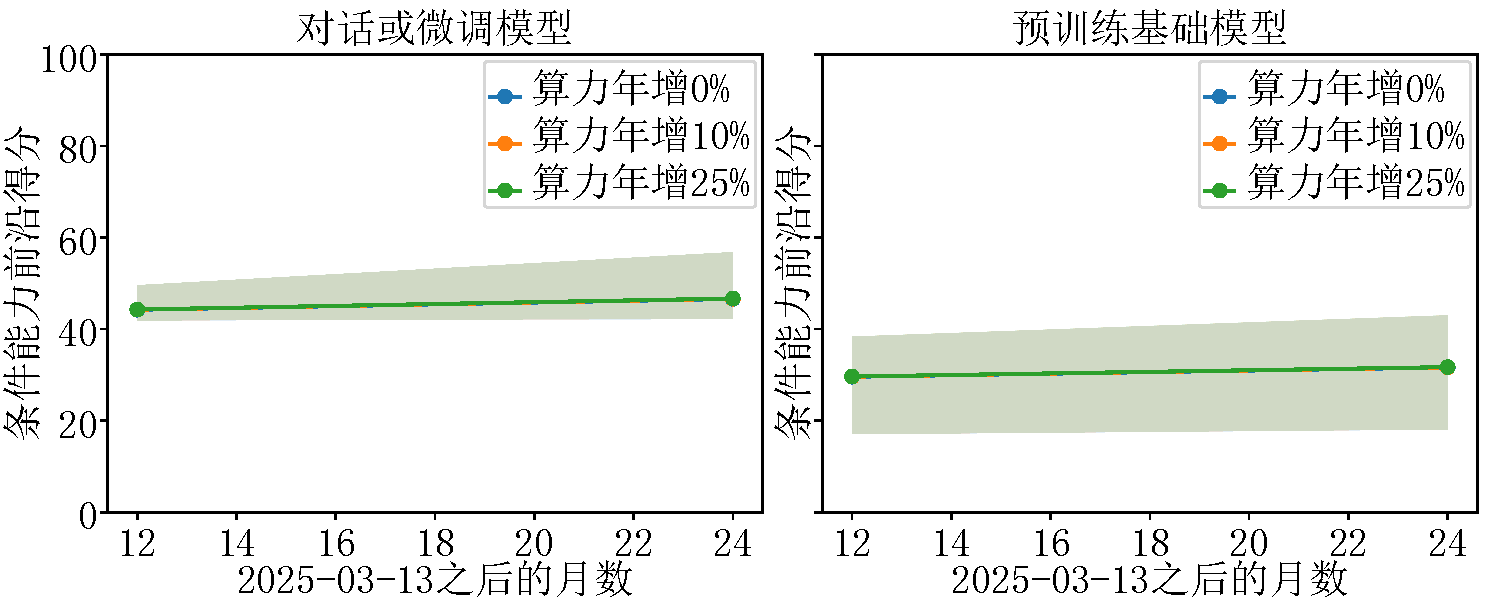
\includegraphics[width=\linewidth]{figures/q4_fig03_frontier_scenarios.pdf}
%         % \caption{算力增长放缓情景下的条件能力前沿预测}
%         % \label{fig:p4_forecast}
%         % \end{figure}

%         % 本次 135 个未来资源配置均超出 B1 的部分支持范围，540 个能力预测的 Loss 也都低于 High 桥接观测范围；阴影仅是当前模型和重采样层次下的条件区间，不是已经校准覆盖率的真实未来预测区间。结论的可靠性主要受跨族桥接样本少、历史训练数据缺失以及后训练算力未计入等因素限制。

%         在指数型质量成本、$L_{\mathrm{ctx}}=8192$、非规模趋势保留一半的条件下，表\ref{tab:p4_forecast}列出不同年算力增长率下的条件能力前沿预测。预测以 2025 年 3 月 13 日为时间起点，12 个月和 24 个月分别对应 2026 年 3 月 13 日和 2027 年 3 月 13 日。

%         \begin{table}[H]
%             \centering
%             \caption{算力增长放缓情景下的条件能力前沿预测（单位：分）}
%             \label{tab:p4_forecast}
%             \small
%             \setlength{\tabcolsep}{4pt}
%             \renewcommand{\arraystretch}{1.15}
%             \begin{tabular}{@{}lcrcrc@{}}
%                 \toprule
%                 模型类型 & 年算力增长率 & \multicolumn{2}{c}{12 个月} & \multicolumn{2}{c}{24 个月} \\
%                 \cmidrule(lr){3-4}
%                 \cmidrule(lr){5-6}
%                 & & 点预测 & 条件 95\% 区间 & 点预测 & 条件 95\% 区间 \\
%                 \midrule
%                 聊天/微调 & 0\%  & 44.24 & [41.95, 49.53] & 46.61 & [42.26, 56.76] \\
%                           & 10\% & 44.26 & [41.96, 49.53] & 46.65 & [42.30, 56.76] \\
%                           & 25\% & 44.28 & [41.97, 49.54] & 46.69 & [42.35, 56.77] \\
%                 \midrule
%                 预训练    & 0\%  & 29.61 & [17.10, 38.29] & 31.64 & [18.12, 42.94] \\
%                           & 10\% & 29.62 & [17.11, 38.30] & 31.67 & [18.14, 42.96] \\
%                           & 25\% & 29.64 & [17.12, 38.32] & 31.70 & [18.17, 42.98] \\
%                 \bottomrule
%             \end{tabular}
        
%             \vspace{0.5em}
%             \begin{minipage}{\linewidth}
%                 \footnotesize
%                 注：固定指数型质量成本、上下文长度 8192，非规模趋势保留比例为 50\%。区间为当前模型及重采样层次下的条件 Bootstrap 区间，未经真实未来数据的覆盖率校准。
%             \end{minipage}
%         \end{table}
        
%         三种算力增长情景下的预测值十分接近。根据未四舍五入的结果，年算力增长率由 0\% 提高至 25\% 时，聊天/微调模型和预训练模型的 24 个月预测值分别增加约 0.0774 分和 0.0673 分。这一结果主要反映 High 桥接在当前外推区间内对 Loss 变化的分数响应较弱，不能据此推断现实中的算力增长对能力提升影响很小。
        
%         本次 135 个未来资源配置均超出 B1 的部分支持范围，540 个能力预测的 Loss 也都低于 High 桥接观测范围。表中区间仅是当前模型和重采样层次下的条件区间，不是已经校准覆盖率的真实未来预测区间。结论的可靠性主要受跨族桥接样本少、历史训练数据缺失以及后训练算力未计入等因素限制。

%         为落实 C8 的逐任务聚合要求，本文读取各模型目录中的原始评测记录，选取截至 2025 年 3 月 13 日最新可解析的文件，跳过损坏文件并记录处理情况。提取每个模型的 24 项 BBH 子任务成绩，分别计算任务宏平均和任务微平均。在符合主分析筛选口径的 574 个模型中，两种聚合得分的模型间均值分别为 46.105 分和 45.870 分，逐模型得分的平均绝对差为 0.235 分，结果表明本样本的总体得分与排序对这两种聚合方式的选择较为稳定。

\section{问题四}   % 7
    \subsection{问题分析}

    前三问最终输出的是验证 Loss，而问题四使用开放模型的六项任务成绩，因此首先需要建立 Loss 到能力分数的可比桥接。历史模型的训练数据量、参数量和发布时间又存在缺失与口径差异，若直接把分数随年份的上升归因于某项技术，会混淆规模扩张、模型族构成和评测选择。本文借鉴观察型标度分析中控制规模与模型族差异的思想\textsuperscript{\cite{ruan2024observational}}，先构造参考规模 Loss，再用时间残差表示未被规模解释的共同变化。

    分数经过 logit 变换后建模，以避免有界指标在线性外推中超过 $[0,100]$。同时，评分口径本身可能改变表观能力曲线\textsuperscript{\cite{schaeffer2023emergent}}，故 C6 桥接按可比性分层，C3 旧口径分数不与主回归直接混合。最终预测以附件截止日前三个月的 95\% 分位前沿为锚点，只解释为外生算力情景下的条件结果。

    \subsection{模型建立}

        % 【补充1】明确开放筛选规则、模型类型、C4 字段用途和时间轴口径。
        \subsubsection{数据筛选、来源匹配与时间口径}
        本文采用可复现的开放权重与许可证代理口径筛选模型：C1 的许可证属于预设白名单，或 C4 的开放权重字段标记为 Yes 时，允许纳入候选样本；若 C4 明确标记为 No，则予以排除。许可证白名单为 Apache-2.0、MIT、BSD-2-Clause、BSD-3-Clause、CC-BY-4.0、CC-BY-SA-4.0、CC0-1.0、GPL-3.0、GPL-2.0、Unlicense 和 WTFPL。许可证不在白名单且权重开放状态未获确认的记录不纳入。上述规则依据附件中的许可标签与权重信息操作，未逐条核验许可证全文及具体使用条件，故本文所称开放模型不等同于经严格开源定义审查的模型。

        根据 C1 的模型类型字段，将基础预训练与持续预训练模型归入 pretrained，将聊天指令模型与微调模型归入 chat/finetuned；合并模型、多模态模型及其他无法归类的记录不进入主比较。进一步要求模型参数量有效、六项任务分数完整且位于 $[0,100]$、提交日期不晚于附件截止日期，并对模型名称去重。两类模型作为历史回归中的类型控制变量，未来前沿也分别报告。

        C1 与 C4 通过规范化模型名称连接。C4 的训练数据量用于构造参考 Loss，训练 FLOPs 用于历史样本筛选、预算基准和算力趋势分析，开放权重字段用于筛选，发布日期用于历史动力学，参数量及其备注用于核对 C1 参数口径并识别 MoE 或激活参数歧义。同名 C4 记录优先选取规模字段最完整者，完整程度相同时选发布日期较早者；匹配后的同一模型镜像保留最早提交记录。主分解样本要求 $N,D,C$ 有效且 C4 明示权重开放，在 C4 参数量可核对时允许与 C1 参数量存在 25\% 的相对偏差，并排除不适用于密集模型标度式的记录；不采用 $D=C/(6N)$ 补齐缺失训练数据量。名称匹配仍可能存在版本错配，其影响列入数据局限。

        历史贡献分解以 C4 的模型发布日期为时间轴，月度榜单前沿与近期前沿锚点以 C1 的提交日期为时间轴，统一以 2025 年 3 月 13 日为附件截止时点。因此，本文的历史分析是使用共同评测基准回顾不同发布日期模型的表现，提交时间不等同于技术出现时间，也不能将其视为历史当时实时可得的排行榜。C3 单独用于来源与年份汇总、与 C1 的重复检查及来源内趋势敏感性分析，避免将旧文献记录直接并入主回归。

        \subsubsection{综合能力与参考规模项}
        对 IFEval、BBH、MATH Lvl 5、GPQA、MUSR 和 MMLU-PRO 六项任务取等权平均：
        \begin{equation}
        S_i=\frac16\sum_{k=1}^{6}s_{ik},\qquad
        z(S)=\operatorname{logit}\!\left[\operatorname{clip}(S/100,0.001,0.999)\right].
        \label{eq:p4_score}
        \end{equation}
        由于历史模型通常缺少逐模型质量和配比，统一在参考条件下计算
        \begin{equation}
        L_i^{ref}=E+A(N_i/10^9)^{-\alpha}+B(D_i/10^{11})^{-\beta}.
        \label{eq:p4_reference_loss}
        \end{equation}
        未观测的数据质量和配比差异留在残差中，不声称已经被控制。

        \subsubsection{单调 Loss--Benchmark 桥接}
        对任务 $k$ 建立带模型类型和模型族控制的岭回归：
        \begin{equation}
        z(s_{ik})=a_k-b_kL_i+c_kI_i^{chat}+\sum_{f\ne f_0}u_{kf}I_{if}+e_{ik},\qquad b_k\ge0.
        \label{eq:p4_bridge}
        \end{equation}
        High 主模型只使用 7 个高可比 Pythia 样本；High+Medium 模型仅作跨族敏感性。参考综合桥接为
        \begin{equation}
        H(L)=\frac{100}{6}\sum_{k=1}^{6}\sigma(a_k-b_kL),\qquad G(L)=z[H(L)].
        \label{eq:p4_bridge_function}
        \end{equation}

        \subsubsection{非规模时间动力学与贡献分解}
        扣除参考规模项后定义
        \begin{equation}
        r_i=z(S_i)-G(L_i^{ref})
        =a+\tau t_i+\delta I_i^{chat}+\sum_{f\ne f_0}v_fI_{if}+\varepsilon_i,
        \label{eq:p4_dynamics}
        \end{equation}
        % 【补充2】明确 t_i 的日期来源、单位及早晚组划分，补出 F 的定义。
        其中 $t_i$ 为模型发布日期距附件截止日期的时间差，以 365.25 天折算为一年，截止日前发布的模型取负值；模型族按记录数倒数加权，并将样本权重归一化至均值为 1。$\tau$ 包含未测质量、架构、对齐、污染和样本选择等共同影响，故称为非规模时间趋势。

        按主样本发布日期的下、上四分位划分早期组和后期组，分别取组内平均参考 Loss $\ell_0,\ell_1$ 与平均时点 $t_0,t_1$，作为早晚组状态。令 $w_i$ 为归一化样本权重，固定完整样本的模型族与类型组成，定义参考 Loss 为 $\ell$、时间为 $t$ 时的预测均值：
        \begin{equation}
        F(\ell,t)=\frac{\sum_i w_i\,100\sigma\!\left[G(\ell)+a+\tau t+\delta I_i^{chat}+\sum_{f\ne f_0}v_fI_{if}\right]}{\sum_i w_i}.
        \label{eq:p4_counterfactual_mean}
        \end{equation}
        对早晚组状态 $(\ell_0,t_0)$ 与 $(\ell_1,t_1)$，采用两因素 Shapley 分解：
        \begin{equation}
        \begin{aligned}
        \Delta_{scale}&=\tfrac12\{F(\ell_1,t_0)-F(\ell_0,t_0)+F(\ell_1,t_1)-F(\ell_0,t_1)\},\\
        \Delta_{time}&=\tfrac12\{F(\ell_0,t_1)-F(\ell_0,t_0)+F(\ell_1,t_1)-F(\ell_1,t_0)\}.
        \end{aligned}
        \label{eq:p4_shapley}
        \end{equation}
        两者之和严格等于模型反事实总变化，且消除了人为规定先改变规模还是先改变时间的顺序依赖。贡献占比分别以两项贡献除以反事实总变化计算，仅在总变化大于 $10^{-6}$ 时报告；两项作用方向相反时允许出现负占比或超过 100\% 的占比，不作截断。该分解针对固定模型族和类型组成后的模型预测变化，不是原始早晚组榜单均值差的直接分解，也不识别具体技术的因果贡献。

        \subsubsection{算力情景与能力前沿预测}
        % 【补充3】补入 C0、趋势系数、前沿锚点、放缓依据与区间传播范围。
        取截止日前一年 C4 中开放语言模型训练 FLOPs 的 95\% 分位为 $C_0$，本次得到 $C_0=7.85865\times10^{24}$ FLOPs，设
        \begin{equation}
        C(h;g)=C_0(1+g)^{h/12},\qquad g\in\{0,0.10,0.25\},\quad h\in\{12,24\}.
        \label{eq:p4_compute_path}
        \end{equation}
        为说明算力增长放缓的设定依据，对截止日前三年 C4 开放语言模型的季度训练 FLOPs 的 95\% 分位拟合对数线性时间趋势，仅使用至少有 3 条记录的季度，得到样本内隐含年增长率约为 254.31\%；因而设定的 0\%、10\% 和 25\% 均低于该描述性历史趋势。该历史增速受模型披露和样本构成影响，不代表行业真实算力增长的精确测量。C4 的训练 FLOPs 用于给出预算数量级，问题三预算则包含训练、质量处理和注意力开销，将二者衔接属于情景假设，未知后训练与部署算力未计入。

        将各预算输入问题三求解器得到最优 Loss $L^*(C)$。将截止日前三个月第 $b$ 类模型综合分的 95\% 分位定义为操作性前沿 $F_{b,0}$，聊天/微调模型和预训练模型的锚点分别为 41.8984 分和 27.6528 分。该前沿反映近期高分模型的分布位置，不等同于理论可达到的绝对最高分。以该前沿为锚点，预测
        \begin{equation}
        \widehat F_b(h)=100\sigma\!\left[z(F_{b,0})+G(L^*(C(h)))-G(L^*(C_0))
        +\rho\widehat\tau h/12\right],\quad \rho\in\{0,0.5,1\}.
        \label{eq:p4_forecast}
        \end{equation}
        其中 $\rho$ 表示非规模趋势停止、保留一半或完全延续，拟合得到的年度 logit 趋势系数为 $\widehat\tau=0.19125$。问题三联合调整 $N,D,Q$，故预测中的 Loss 改善项表示预算变化后资源配置的综合收益；历史贡献分解则固定质量与配比的参考条件，二者口径不同。未来质量投资收益与非规模时间趋势可能部分重叠，本文通过 $\rho$ 的敏感性情景展示这一假设的影响。

        采用 200 次分层 Bootstrap 传播桥接、模型族、前沿锚点和问题二参数的不确定性\textsuperscript{\cite{efron1979bootstrap}}。重采样分别作用于 High 桥接模型、历史模型族与分类型前沿锚点，并抽取问题二参数重新计算 Loss；问题三部分仅在已求得的最优配置上重算 Loss，不在每次重采样中重新优化。因此，所得区间是给定模型形式和优化配置下的条件区间，未覆盖最优配置重新选择、质量迁移机制及未来技术冲击等全部不确定性。

        \subsubsection{逐任务聚合分析}
        % 【补充4】明确 C8 指标字段与有效样本数的处理规则。
        定义 $\mathcal K_i$ 为模型 $i$ 对应于 C8 的 BBH 叶子子任务集合，$a_{ik}$ 为模型 $i$ 在第 $k$ 个子任务的原始评测字段 \texttt{acc\_norm,none} 所记录的正确率，范围为 $0\sim1$，$n_{ik}$ 为相应样本数。样本数优先取 \texttt{effective}，缺失时取 \texttt{original}，均缺失或最终数值无效时取 1；保留原始记录供核对，并排除 BBH 汇总父节点以避免重复计数。定义任务宏平均和任务微（加权）平均：
        \begin{equation}
        B_i^{macro}=\frac{100}{|\mathcal K_i|}\sum_{k\in\mathcal K_i}a_{ik},\qquad
        B_i^{micro}=100\frac{\sum_{k\in\mathcal K_i} n_{ik}a_{ik}}{\sum_{k\in\mathcal K_i} n_{ik}}.
        \label{eq:p4_aggregation}
        \end{equation}

    \subsection{建模结果}

        截止 2025 年 3 月 13 日，4576 条 C1 记录经开放口径、模型类型和字段有效性筛选后保留 1329 个模型，其中 52 个具有可用于参考规模项的完整密集模型记录；C6 High 桥接样本为 7 个。

        % 【补充5】加入 C3 实际使用结果与来源内趋势敏感性表。
        C3 共包含 4599 条记录，其中 4573 条榜单记录的模型名称与 C1 重合，另外 26 条来自历史论文或报告。历史来源中，\texttt{Average} 与六任务均值的最大绝对差达到 42.3333 分，说明不同来源记录不能直接视为同一综合能力指标。为检验来源差异，分别在各来源内以 \texttt{Average} 经 logit 变换后的分数为因变量、对数参数量和年份为自变量拟合岭回归，结果见表\ref{tab:p4_c3_sensitivity}。两类来源的时间系数方向不同，反映出历史条目的构成与评分口径对趋势判断的影响，支持将 C3 用于来源内描述性敏感性分析而不直接混入主回归；这些系数不用于跨来源比较技术进步速度，历史来源的负系数也不能解释为技术退步。

        \begin{table}[H]
        \centering
        \caption{C3 的来源内趋势敏感性分析}
        \label{tab:p4_c3_sensitivity}
        \begin{tabular}{lrrr}
        \toprule
        数据来源 & 原始记录数 & 有效拟合数 & 年度 logit 趋势系数 \\
        \midrule
        历史论文/报告 & 26 & 26 & $-0.02952$ \\
        Open LLM Leaderboard & 4573 & 4566 & $0.17460$ \\
        \bottomrule
        \end{tabular}
        % \vspace{0.5em}
        % \begin{minipage}{\linewidth}
        % \footnotesize
        % 注：有效拟合样本要求参数量为正、Average 位于 $[0,100]$ 且年份非缺失；来源内模型控制对数参数量。该分析保留各来源自身的分数口径，仅用于描述性敏感性比较。
        % \end{minipage}
        \end{table}

        图\ref{fig:p4_bridge}给出分层桥接。High 留一 MAE 为 0.3335 分，略低于均值基线的 0.3756 分；跨族敏感性桥接 MAE 为 10.8775 分，高于均值基线的 10.3411 分，说明跨族映射仍不稳定。

        \begin{figure}[H]
        \centering
        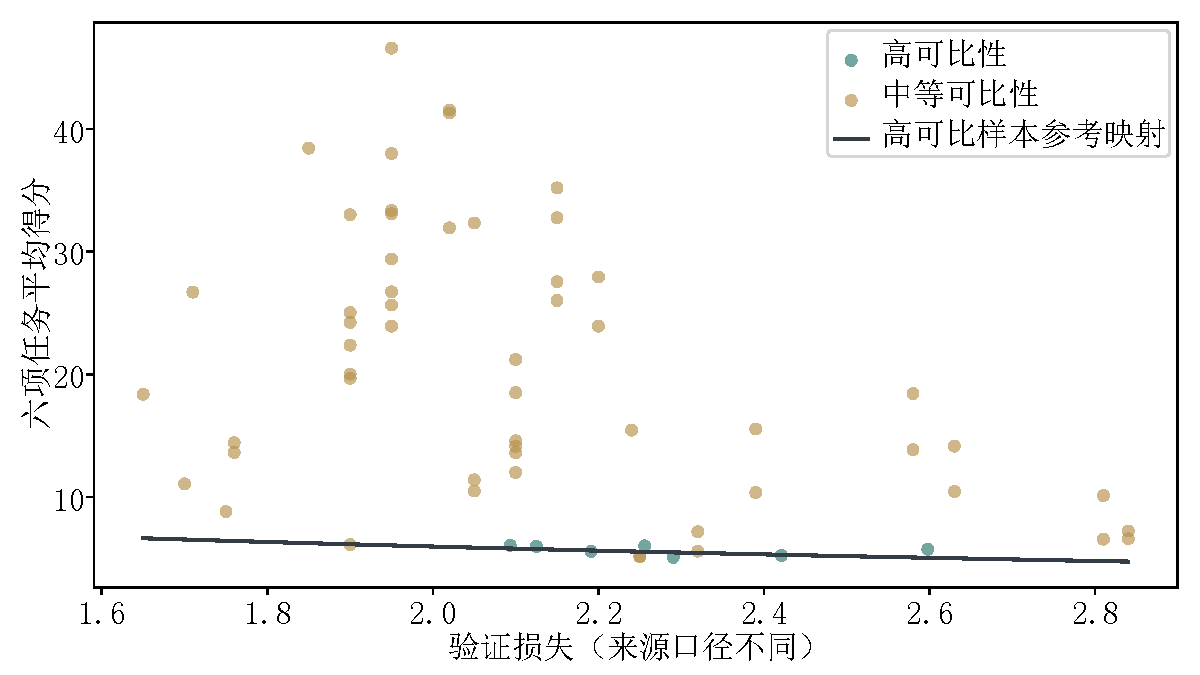
\includegraphics[width=0.86\linewidth]{figures/q4_fig01_loss_benchmark_bridge.pdf}
        \caption{分层 Loss--Benchmark 桥接及高可比参考映射}
        \label{fig:p4_bridge}
        \end{figure}

        \begin{table}[H]
        \centering
        \caption{问题四桥接与时间留出检验}
        \label{tab:p4_validation}
        \begin{tabular}{lrrr}
        \toprule
        检验 & 样本量 & MAE & 均值基线 MAE \\
        \midrule
        High 按模型留一 & 7 & 0.3335 & 0.3756 \\
        High+Medium 按族留一 & 62 & 10.8775 & 10.3411 \\
        60\% 时间截断 & 21 & 11.1606 & 11.1585 \\
        75\% 时间截断 & 11 & 12.6152 & 12.7228 \\
        85\% 时间截断 & 8 & 14.3541 & 14.1148 \\
        \bottomrule
        \end{tabular}
        % 【补充6】说明时间检验固定桥接，避免与全流程历史回测混淆。
        % \vspace{0.5em}
        % \begin{minipage}{\linewidth}
        % \footnotesize
        % 注：时间截断按主样本发布日期的相应分位划分，前段拟合动力学、后段检验；C6 桥接保持固定。因此该检验是回顾性的动力学时间留出，未重建各截点当时可获得的完整信息。
        % \end{minipage}
        \end{table}

        图\ref{fig:p4_history}展示每月新增提交模型的 95\% 分位，而非历史累计最高值，因此曲线允许下降。三个时间留出误差也未稳定优于均值基线，说明预测应理解为结构化情景而非高精度长期预测器。

        \begin{figure}[H]
        \centering
        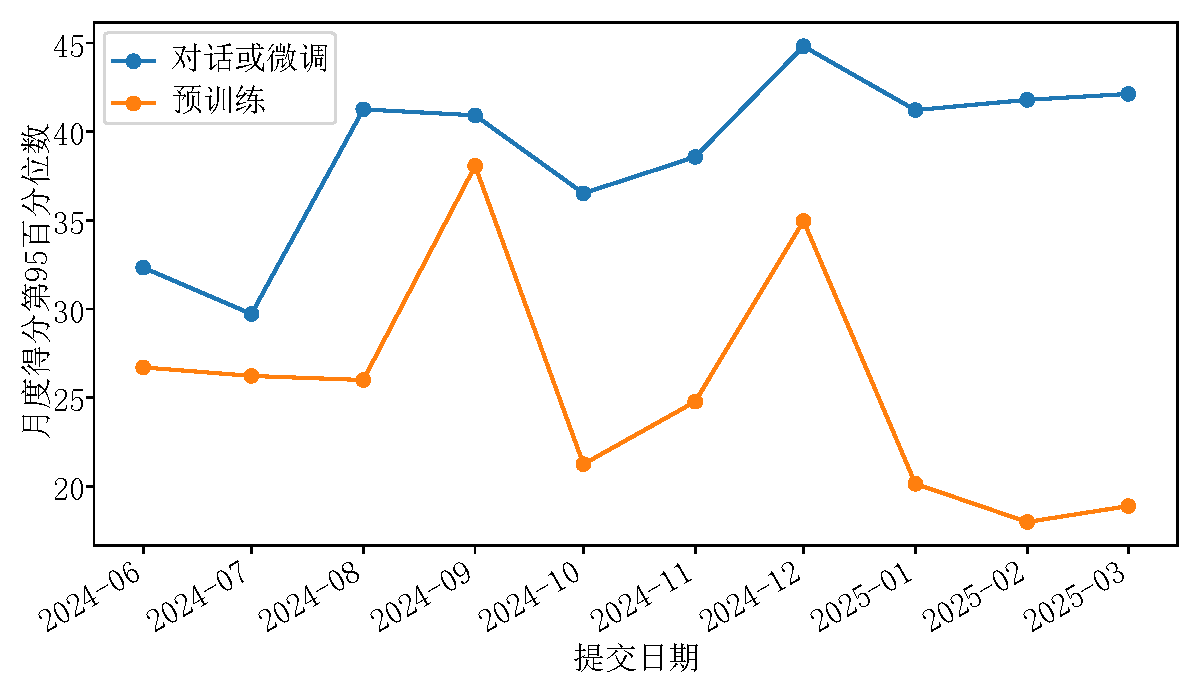
\includegraphics[width=0.88\linewidth]{figures/q4_fig02_historical_frontier.pdf}
        \caption{开放模型六任务综合能力的月度操作性前沿}
        \label{fig:p4_history}
        \end{figure}

        条件 Shapley 点估计给出早晚组在固定模型族与类型组成下的反事实总变化为 3.7429 分，其中规模项 0.3380 分、非规模时间项 3.4048 分，占比分别为 9.03\% 和 90.97\%。规模项的 Bootstrap 95\% 区间为 $[-0.1420,0.6848]$ 分，对应占比区间约为 $[-2.80\%,36.83\%]$；因此不能把 90.97\% 写成已经识别的技术因果贡献。

        在指数型质量成本、$L_{\mathrm{ctx}}=8192$、非规模趋势保留一半的条件下，表\ref{tab:p4_forecast}列出不同年算力增长率下的条件能力前沿预测。预测以 2025 年 3 月 13 日为时间起点，12 个月和 24 个月分别对应 2026 年 3 月 13 日和 2027 年 3 月 13 日。

        \begin{table}[H]
            \centering
            \caption{算力增长放缓情景下的条件能力前沿预测（单位：分）}
            \label{tab:p4_forecast}
            \small
            \setlength{\tabcolsep}{4pt}
            \renewcommand{\arraystretch}{1.15}
            \begin{tabular}{@{}lcrcrc@{}}
                \toprule
                模型类型 & 年算力增长率 & \multicolumn{2}{c}{12 个月} & \multicolumn{2}{c}{24 个月} \\
                \cmidrule(lr){3-4}
                \cmidrule(lr){5-6}
                & & 点预测 & 条件 95\% 区间 & 点预测 & 条件 95\% 区间 \\
                \midrule
                聊天/微调 & 0\%  & 44.24 & [41.95, 49.53] & 46.61 & [42.26, 56.76] \\
                          & 10\% & 44.26 & [41.96, 49.53] & 46.65 & [42.30, 56.76] \\
                          & 25\% & 44.28 & [41.97, 49.54] & 46.69 & [42.35, 56.77] \\
                \midrule
                预训练    & 0\%  & 29.61 & [17.10, 38.29] & 31.64 & [18.12, 42.94] \\
                          & 10\% & 29.62 & [17.11, 38.30] & 31.67 & [18.14, 42.96] \\
                          & 25\% & 29.64 & [17.12, 38.32] & 31.70 & [18.17, 42.98] \\
                \bottomrule
            \end{tabular}
            % \vspace{0.5em}
            % \begin{minipage}{\linewidth}
            %     \footnotesize
            %     注：固定指数型质量成本、上下文长度 8192，非规模趋势保留比例为 50\%。区间为当前模型及重采样层次下的条件 Bootstrap 区间，未经真实未来数据的覆盖率校准。
            % \end{minipage}
        \end{table}

        三种算力增长情景下的预测值十分接近。根据未四舍五入的结果，年算力增长率由 0\% 提高至 25\% 时，聊天/微调模型和预训练模型的 24 个月预测值分别增加约 0.0774 分和 0.0673 分。这一结果主要反映 High 桥接在当前外推区间内对 Loss 变化的分数响应较弱，不能据此推断现实中的算力增长对能力提升影响很小。

        % 【补充7】加入 rho=0、0.5、1 的已有敏感性结果，其他条件与原预测一致。
        为考察非规模趋势延续假设的影响，在指数型质量成本、$L_{\mathrm{ctx}}=8192$ 和年算力增长率 10\% 下，进一步比较 $\rho=0,0.5,1$ 三种情景，结果见表\ref{tab:p4_retention_sensitivity}。三种趋势情景为外生假设，未赋予发生概率，表中仅列条件点预测。当趋势停止时，两类模型的预测前沿接近当前锚点；当趋势完全延续时，聊天/微调模型和预训练模型的 24 个月预测分别达到 51.42 分和 35.94 分。在当前模型中，趋势保留比例引起的预测差异大于三种算力增速之间的差异，说明条件预测主要受非规模趋势能否延续的假设影响，该结果不能据此推广为现实中技术与算力作用大小的因果排序。

        \begin{table}[H]
        \centering
        \caption{非规模趋势保留比例的条件预测敏感性（单位：分）}
        \label{tab:p4_retention_sensitivity}
        \begin{tabular}{lcrr}
        \toprule
        模型类型 & 趋势保留比例 $\rho$ & 12 个月 & 24 个月 \\
        \midrule
        聊天/微调 & 0 & 41.91 & 41.93 \\
                  & 0.5 & 44.26 & 46.65 \\
                  & 1 & 46.63 & 51.42 \\
        \midrule
        预训练    & 0 & 27.67 & 27.68 \\
                  & 0.5 & 29.62 & 31.67 \\
                  & 1 & 31.65 & 35.94 \\
        \bottomrule
        \end{tabular}
        % \vspace{0.5em}
        % \begin{minipage}{\linewidth}
        % \footnotesize
        % 注：固定指数型质量成本、上下文长度 8192 和年算力增长率 10\%；三种趋势情景为外生假设，未赋予发生概率，表中仅列条件点预测。
        % \end{minipage}
        \end{table}

        本次 135 个资源配置均超出 B1 的部分支持范围，540 个能力预测的 Loss 也都低于 High 桥接观测范围。表\ref{tab:p4_forecast}中区间仅是当前模型和重采样层次下的条件区间，不是已经校准覆盖率的真实未来预测区间。结论的可靠性主要受跨族桥接样本少、历史训练数据缺失以及后训练算力未计入等因素限制。

        % 【修订8】区分“宏微平均得分接近”和“C8 宏平均与 C1 榜单排序一致”。
        为落实 C8 的逐任务聚合要求，本文读取各模型目录中的原始评测记录，选取截至 2025 年 3 月 13 日最新可解析的文件，跳过损坏文件并记录处理情况，共获得 1859 个模型的 44616 条 BBH 子任务记录，每个模型包含 24 项子任务。在与开放筛选后的 C1 样本匹配的 574 个模型中，任务宏平均和任务微平均的模型间均值分别为 46.105 分和 45.870 分，两均值相差约 0.235 分，逐模型得分的平均绝对差为 0.237 分，说明本样本的聚合得分对这两种加权方式的选择较为稳定。进一步比较 C8 子任务宏平均与 C1 榜单 BBH 得分，Spearman 秩相关系数为 0.997334，说明两种数据来源的模型排序具有较高一致性；该系数比较的是 C8 宏平均与 C1 榜单得分，不是宏平均与微平均之间的排序相关。由于原始任务正确率与榜单变换分数的口径不同，二者不直接作数值差来衡量预测误差。


\section{模型评价}  % 8 (1~3 pages)
    \subsection{模型的优点}
    （1）模型衔接明确，兼顾整体分析与分阶段检验。
    本文围绕数据质量与领域配比、训练损失、资源配置和任务能力建立递进模型，各阶段通过明确的评分、响应函数与优化结果传递信息，形成从数据评价到资源决策的完整分析框架。各模块又可分别开展验证与参数更新，便于定位误差来源，并在新增数据条件下进行修正。
    
    （2）针对数据结构选择方法，兼顾稳健性与可解释性。
    针对质量指标方向不一、尺度不同及相互冲突的问题，采用统一转换、受限 CRITIC 赋权与 Huber 鲁棒估计，限制异常指标对综合评分的影响。针对领域份额总和为一的约束，采用 ILR 变换与二次多输出岭回归刻画配比效应。同规模检验的决定系数约为 0.86，表明模型能够较好地解释观测范围内的配比差异；二次项及边际效应分析也为领域组合关系提供了解释依据。
    
    （3）标度关系与算力约束相结合，能够支持资源投入比较。
    广义标度律保留经典双幂律的参考结构，并通过配比相对响应和额外质量修正区分不同因素的作用。由此推导的边际收益、弹性与等效替代条件，可用于比较扩充参数、增加数据和提高质量的收益。进一步将基础训练、质量提升及长上下文开销纳入统一预算，通过降维求解和多情景比较，能够分析不同成本条件下资源配置的变化。

    \subsection{模型的不足}
    （1）质量量尺与跨来源映射仍存在不确定性。
    综合质量分由自动评价信号构成，其与实际训练收益之间的对应关系仍缺少充分的独立标定。不同领域的文本特征也可能使统一转换规则产生偏差。质量领域与配方领域映射不完整，加之不同来源的训练和评测口径存在差异，限制了质量、配比与规模效应的独立识别及跨规模迁移。
    
    （2）成本与收益的刻画有所简化，优化结论具有条件性。
    问题三主要依据题设成本函数描述算力消耗，尚未充分考虑硬件利用率、通信和后训练开销；上下文长度主要通过成本影响资源配置，其对任务表现的直接收益尚未纳入。网格搜索与 SLSQP 求解也未提供连续可行域内的全局最优证明，经验候选配方的比较范围有限，因此所得方案依赖既定成本形式、变量范围与候选集合。
    
    （3）多阶段误差传递与能力外推仍需加强验证。
    前序质量评分、配比响应和标度律参数的偏差，可能经资源优化与能力桥接传递至最终预测。现有 Bootstrap 已覆盖部分参数与抽样不确定性，但尚未完整覆盖模型形式、成本设定及重新优化带来的不确定性。此外，第四问高可比桥接样本较少，跨模型族及时间留出结果未稳定优于均值基线，未来情景又超出部分观测范围，因此能力分数应作为条件预测解释，非规模时间贡献也不能直接等同于技术进步的因果贡献。

    \subsection{模型的改进方向}
    （1）补充质量标定与可比对照实验。
    针对质量量尺与效应识别不足，可按领域抽取文本开展人工复核，并结合小规模训练实验校准质量评分。在固定规模和配比时改变质量、固定规模和质量时改变配比，通过控制变量提高各因素作用的可辨识性；同时统一评测口径，补充跨规模验证数据。
    
    （2）利用实测成本完善资源优化。
    通过训练日志标定不同硬件、上下文长度及数据处理方式下的实际开销，并逐步纳入后训练成本与长上下文任务收益。对资源配置发生明显变化的预算区间加密搜索，结合多起点求解和参数扰动检验，评估候选方案的稳定性；进一步采用多情景或稳健优化，降低方案对单一成本假设的依赖。
    
    （3）开展全流程不确定性传播与滚动验证。
    可在重采样后重新估计前序模型、求解资源配置并计算能力预测，检查不确定性在四个阶段中的累积与传递。同时补充不同模型族的损失—能力配对记录，采用滚动时间留出检验评估预测误差，并随新增数据更新桥接关系和前沿锚点，提高情景分析的可靠性。

\clearpage

\bibliographystyle{gmcm}
\bibliography{reference}

% % 以下旧的手写参考文献块不再参与编译，仅暂存以便核对迁移是否完整。
% \iffalse
% \begin{thebibliography}{99}
%  \bibitem{wettig2024qurating} Wettig, A., Gupta, A., Malik, S., Chen, D. 2024. QuRating: Selecting High-Quality Data for Training Language Models. Proceedings of the 41st International Conference on Machine Learning, PMLR, 235, 52915--52971. \url{https://proceedings.mlr.press/v235/wettig24a.html}. \bibitem{huber1964robust} Huber, P. J. 1964. Robust Estimation of a Location Parameter. The Annals of Mathematical Statistics, 35(1), 73--101. \url{https://doi.org/10.1214/aoms/1177703732}. \bibitem{aitchison1982compositional} Aitchison, J. 1982. The Statistical Analysis of Compositional Data. Journal of the Royal Statistical Society. Series B (Methodological), 44(2), 139--177. \url{https://doi.org/10.1111/j.2517-6161.1982.tb01195.x}. \bibitem{liu2025regmix} Liu, Q., Zheng, X., Muennighoff, N., Zeng, G., Dou, L., Pang, T., Jiang, J., Lin, M. 2025. RegMix: Data Mixture as Regression for Language Model Pre-training. The Thirteenth International Conference on Learning Representations (ICLR). \url{https://arxiv.org/abs/2407.01492}. \bibitem{egozcue2003ilr} Egozcue, J. J., Pawlowsky-Glahn, V., Mateu-Figueras, G., Barcel\'o-Vidal, C. 2003. Isometric Logratio Transformations for Compositional Data Analysis. Mathematical Geology, 35(3), 279--300. \url{https://doi.org/10.1023/A:1023818214614}. \bibitem{hoerl1970ridge} Hoerl, A. E., Kennard, R. W. 1970. Ridge Regression: Biased Estimation for Nonorthogonal Problems. Technometrics, 12(1), 55--67. \url{https://doi.org/10.1080/00401706.1970.10488634}. \bibitem{diakoulaki1995critic} Diakoulaki, D., Mavrotas, G., Papayannakis, L. 1995. Determining objective weights in multiple criteria problems: The CRITIC method. Computers \& Operations Research, 22(7), 763--770. \url{https://doi.org/10.1016/0305-0548(94)00059-H}.
 
% \bibitem{hoffmann2022chinchilla} Hoffmann, J., Borgeaud, S., Mensch, A., et al. 2022. An empirical analysis of compute-optimal large language model training. Advances in Neural Information Processing Systems, 35. \url{https://proceedings.neurips.cc/paper_files/paper/2022/hash/c1e2faff6f588870935f114ebe04a3e5-Abstract.html}. \bibitem{ye2025mixing} Ye, J., Liu, P., Sun, T., Zhan, J., Zhou, Y., Qiu, X. 2025. Data Mixing Laws: Optimizing Data Mixtures by Predicting Language Modeling Performance. The Thirteenth International Conference on Learning Representations (ICLR). \url{https://arxiv.org/abs/2403.16952}. \bibitem{biderman2023pythia} Biderman, S., Schoelkopf, H., Anthony, Q. G., et al. 2023. Pythia: A Suite for Analyzing Large Language Models Across Training and Scaling. Proceedings of the 40th International Conference on Machine Learning, PMLR, 202, 2397--2430. \url{https://proceedings.mlr.press/v202/biderman23a.html}. \bibitem{subramanyam2026quality} Subramanyam, A., Chen, Y., Grossman, R. L. 2026. Scaling Laws Revisited: Modeling the Role of Data Quality in Language Model Pretraining. The Fourteenth International Conference on Learning Representations (ICLR). \url{https://arxiv.org/abs/2510.03313}. \bibitem{virtanen2020scipy} Virtanen, P., Gommers, R., Oliphant, T. E., et al. 2020. SciPy 1.0: Fundamental Algorithms for Scientific Computing in Python. Nature Methods, 17(3), 261--272. \url{https://doi.org/10.1038/s41592-019-0686-2}. \bibitem{efron1979bootstrap} Efron, B. 1979. Bootstrap Methods: Another Look at the Jackknife. The Annals of Statistics, 7(1), 1--26. \url{https://doi.org/10.1214/aos/1176344552}. \end{thebibliography}


\fi

% \clearpage


% \begin{appendices}  % 附录
%     % \setcounter{page}{1}  % 如果需要可以自行重置页码。
%     \section{MATLAB 源程序}    % 附录 A
%     \renewcommand{\thesubsection}{A\thinskip.\thinskip\arabic{subsection}}
%         \subsection{第1问程序}  % A.1
%         \vspace{-2ex}
        
%         \begin{Matlab}{code.m}
%         clear all
%         kk=2;
%         [mdd,ndd]=size(dd);
%         while ~isempty(V)
%             [tmpd,j]=min(W(i,V));
%             tmpj=V(j);
%             for k=2:ndd
%                 [tmp1,jj]=min(dd(1,k)+W(dd(2,k),V));
%                 tmp2=V(jj);
%                 tt(k-1,:)=[tmp1,tmp2,jj];
%             end
%             tmp=[tmpd,tmpj,j;tt];
%             [tmp3,tmp4]=min(tmp(:,1));
%             if tmp3==tmpd,
%                 ss(1:2,kk)=[i;tmp(tmp4,2)];
%             else
%                 tmp5=find(ss(:,tmp4)~=0);
%                 tmp6=length(tmp5);
%                 if dd(2,tmp4)==ss(tmp6,tmp4)
%                     ss(1:tmp6+1,kk)=[ss(tmp5,tmp4);tmp(tmp4,2)];
%                 else, ss(1:3,kk)=[i;dd(2,tmp4);tmp(tmp4,2)];
%                 end
%             end
%             dd=[dd,[tmp3;tmp(tmp4,2)]];
%             V(tmp(tmp4,3))=[];
%             [mdd,ndd]=size(dd);kk=kk+1;
%         end;
%         S=ss; D=dd(1,:);
%         \end{Matlab}
%         \vspace{2ex}
    

% 用法：替换原稿从 Python 源程序前的 \clearpage 到 \end{appendices} 的整段。
% 原稿须已处于 appendices 环境内，且已定义 Python 代码环境。
\clearpage
\section{Python 源程序}    % 附录 B
\renewcommand{\thesubsection}{A\thinskip.\thinskip\arabic{subsection}}
\setcounter{subsection}{0}

% 仅调整本附录的代码排版：允许长表达式、字符串在灰色框内自动折行。
% 不沿用原行的深层缩进，避免续行被挤出右边界；不改变 Python 代码内容。
\begingroup
\lstset{
    linewidth=\linewidth,
    columns=fullflexible,
    keepspaces=true,
    breaklines=true,
    breakatwhitespace=false,
    breakautoindent=false,
    breakindent=1em,
    prebreak={},
    postbreak={}
}

本附录列出第 1--4 问的核心计算代码，省略原始数据读取、绘图和批量结果输出等辅助流程。
代码中的辅助函数、字段定义和参数结构沿用对应的完整源程序；导入路径以项目根目录为基准。
所有数值计算均使用 \texttt{modeling-q1} 环境。第 4 问采用与正文一致的原版模型。

\subsection{第1问程序}  % B.1
质量指标方向统一、受限 CRITIC 权重、Huber 鲁棒评分与冲突识别，以及 ILR 二次岭回归和五折选参。

\vspace{-2ex}
\begin{Python}{problem1\_solution.py（核心节选）}
# 核心节选；辅助函数及输入结构见对应完整源程序。
# 在项目根目录使用 modeling-q1 环境导入这些函数。
from __future__ import annotations
import numpy as np
import pandas as pd
from Problem1.problem1_solution import (
    QUALITY_FIELDS, DIRECTION, helmert_basis, close_composition,
    QuadraticRidgeModel, _ridge_solution,
)


def fit_reference_transform(sample: pd.DataFrame) -> pd.DataFrame:
    rows = []
    for field in QUALITY_FIELDS:
        values = pd.to_numeric(sample[field], errors="coerce").to_numpy(float)
        finite = values[np.isfinite(values)]
        if finite.size < 10:
            raise ValueError(f"指标 {field} 的有效样本不足")
        q01, q50, q99 = np.quantile(finite, [0.01, 0.50, 0.99])
        if not q99 > q01:
            q99 = q01 + 1.0
        rows.append(
            {
                "metric": field,
                "direction": DIRECTION[field],
                "q01": q01,
                "q50": q50,
                "q99": q99,
                "sample_missing_rate": float(np.mean(~np.isfinite(values))),
            }
        )
    return pd.DataFrame(rows).set_index("metric")


def transform_desirability(raw: pd.DataFrame, reference: pd.DataFrame) -> pd.DataFrame:
    out = pd.DataFrame(index=raw.index)
    for field in QUALITY_FIELDS:
        x = pd.to_numeric(raw[field], errors="coerce").to_numpy(float)
        row = reference.loc[field]
        lo, med, hi = float(row.q01), float(row.q50), float(row.q99)
        clipped = np.clip(x, lo, hi)
        direction = row.direction
        if direction == "benefit":
            score = (clipped - lo) / (hi - lo)
        elif direction == "cost":
            score = (hi - clipped) / (hi - lo)
        else:
            left = np.maximum(med - lo, 1e-12)
            right = np.maximum(hi - med, 1e-12)
            score = np.where(clipped <= med, 1.0 - (med - clipped) / left,
                             1.0 - (clipped - med) / right)
        out[field] = np.clip(score, 0.0, 1.0)
    # 先按领域中位数填补，再用 A1 全局中位数兜底；同时另行保留覆盖率。
    domains = raw["domain"]
    for field in QUALITY_FIELDS:
        med_by_domain = out[field].groupby(domains).transform("median")
        out[field] = out[field].fillna(med_by_domain).fillna(out[field].median())
    return out


def critic_weights(sample_scores: pd.DataFrame, blend: float = 0.5) -> pd.Series:
    x = sample_scores[QUALITY_FIELDS].to_numpy(float)
    sd = np.nanstd(x, axis=0, ddof=1)
    corr = np.corrcoef(x, rowvar=False)
    corr = np.nan_to_num(corr, nan=0.0)
    information = sd * np.sum(1.0 - np.abs(corr), axis=1)
    if not np.any(information > 0):
        information = np.ones(len(QUALITY_FIELDS))
    critic = information / information.sum()
    equal = np.full(len(QUALITY_FIELDS), 1.0 / len(QUALITY_FIELDS))
    blend = float(np.clip(blend, 0.0, 1.0))
    blended = (1.0 - blend) * equal + blend * critic
    lower, upper = 0.5 / len(QUALITY_FIELDS), 2.0 / len(QUALITY_FIELDS)
    blended = np.clip(blended, lower, upper)
    blended /= blended.sum()
    return pd.Series(blended, index=QUALITY_FIELDS, name="weight")


def huber_location(x: np.ndarray, weights: np.ndarray, iterations: int = 6) -> np.ndarray:
    base = np.broadcast_to(weights, x.shape)
    mu = np.sum(base * x, axis=1) / np.sum(base, axis=1)
    for _ in range(iterations):
        residual = x - mu[:, None]
        scale = 1.4826 * np.median(np.abs(residual), axis=1) + 1e-6
        ratio = np.abs(residual) / (1.345 * scale[:, None])
        robust = np.where(ratio <= 1.0, 1.0, 1.0 / np.maximum(ratio, 1e-12))
        effective = base * robust
        mu = np.sum(effective * x, axis=1) / np.sum(effective, axis=1)
    return np.clip(mu, 0.0, 1.0)


def score_quality(
    raw: pd.DataFrame,
    critic_blend: float = 0.5,
    conflict_quantile: float = 0.95,
    conflict_spread: float = 0.60,
) -> tuple[pd.DataFrame, pd.DataFrame, pd.DataFrame, pd.DataFrame]:
    sample_mask = raw["dataset"].eq("sample")
    reference = fit_reference_transform(raw.loc[sample_mask])
    scores = transform_desirability(raw, reference)
    weights = critic_weights(scores.loc[sample_mask], critic_blend)
    x = scores[QUALITY_FIELDS].to_numpy(float)
    w = weights.to_numpy(float)
    q = huber_location(x, w)
    disagreement = np.sqrt(np.sum(w[None, :] * (x - q[:, None]) ** 2, axis=1))
    spread = np.quantile(x, 0.90, axis=1) - np.quantile(x, 0.10, axis=1)
    sample_threshold = float(np.quantile(disagreement[sample_mask.to_numpy()], conflict_quantile))
    conflict = (disagreement > sample_threshold) & (spread > conflict_spread)
    coverage = raw[QUALITY_FIELDS].notna().mean(axis=1).to_numpy(float)
    confidence = coverage * (1.0 - np.clip(disagreement / 0.50, 0.0, 1.0))

    record = raw[["id", "dataset", "domain", "source_file"]].copy()
    record["Q"] = q
    record["disagreement"] = disagreement
    record["spread_p90_p10"] = spread
    record["conflict"] = conflict.astype(int)
    record["confidence"] = confidence
    record["coverage"] = coverage

    diagnostics = reference.copy()
    diagnostics["weight"] = weights
    diagnostics["all_missing_rate"] = raw[QUALITY_FIELDS].isna().mean()
    diagnostics["conflict_threshold_disagreement"] = sample_threshold
    diagnostics["critic_blend"] = critic_blend
    diagnostics["conflict_quantile"] = conflict_quantile
    diagnostics["conflict_spread_threshold"] = conflict_spread
    diagnostics = diagnostics.reset_index()

    conflicting_x = x[conflict]
    if conflicting_x.size:
        conflicting_q = q[conflict]
        contrib = np.mean(w[None, :] * np.abs(conflicting_x - conflicting_q[:, None]), axis=0)
        contrib = contrib / max(contrib.sum(), 1e-12)
    else:
        contrib = np.zeros(len(QUALITY_FIELDS))
    contributions = pd.DataFrame(
        {"metric": QUALITY_FIELDS, "weight": w, "conflict_contribution": contrib}
    ).sort_values("conflict_contribution", ascending=False)

    merged = pd.concat([record, scores.add_prefix("S_")], axis=1)
    return merged, diagnostics, contributions, scores


def ilr_transform(p: np.ndarray, pseudocount: float = 1e-4) -> np.ndarray:
    closed = close_composition(p, pseudocount)
    clr = np.log(closed) - np.log(closed).mean(axis=1, keepdims=True)
    basis = helmert_basis(closed.shape[1])
    return clr @ basis.T


def polynomial_features_degree2(z: np.ndarray) -> np.ndarray:
    z = np.asarray(z, float)
    parts = [z]
    for j in range(z.shape[1]):
        parts.append(z[:, j:j + 1] * z[:, j:])
    return np.concatenate(parts, axis=1)


def fit_quadratic_ridge_cv(z: np.ndarray, y: np.ndarray, seed: int = 20260924) -> QuadraticRidgeModel:
    x = polynomial_features_degree2(z)
    alphas = np.logspace(-4, 4, 25)
    rng = np.random.default_rng(seed)
    shuffled = rng.permutation(len(x))
    folds = np.array_split(shuffled, 5)
    errors = np.zeros(len(alphas), dtype=float)
    for valid_idx in folds:
        train_idx = np.setdiff1d(shuffled, valid_idx, assume_unique=True)
        x_train, x_valid = x[train_idx], x[valid_idx]
        y_train, y_valid = y[train_idx], y[valid_idx]
        mean = x_train.mean(axis=0)
        std = x_train.std(axis=0, ddof=0)
        std[std < 1e-12] = 1.0
        xs = (x_train - mean) / std
        xv = (x_valid - mean) / std
        y_mean = y_train.mean(axis=0)
        yc = y_train - y_mean
        gram = xs.T @ xs
        values, vectors = np.linalg.eigh(gram)
        projected = vectors.T @ (xs.T @ yc)
        for ai, alpha in enumerate(alphas):
            coef = vectors @ (projected / (values[:, None] + alpha))
            pred = y_mean + xv @ coef
            errors[ai] += float(np.mean((y_valid - pred) ** 2))
    best_alpha = float(alphas[int(np.argmin(errors))])
    x_mean = x.mean(axis=0)
    x_std = x.std(axis=0, ddof=0)
    x_std[x_std < 1e-12] = 1.0
    xs = (x - x_mean) / x_std
    y_mean = y.mean(axis=0)
    coef = _ridge_solution(xs, y - y_mean, best_alpha)
    return QuadraticRidgeModel(best_alpha, x_mean, x_std, y_mean, coef)
\end{Python}

\subsection{第2问程序}  % B.2
经典标度律的均衡加权拟合、质量响应校准、领域配比桥接，以及质量提升与参数扩容的等效替代计算。

\vspace{-2ex}
\begin{Python}{problem2\_solution.py（核心节选）}
# 核心节选；辅助函数及输入结构见对应完整源程序。
# 在项目根目录使用 modeling-q1 环境导入这些函数。
from __future__ import annotations
import importlib.util
import json
import numpy as np
import pandas as pd
from scipy.optimize import least_squares
from Problem2.problem2_solution import BASE


def nd(frame):
    return frame.N_params_B.to_numpy(float), frame.D_tokens_B.to_numpy(float) / 100.0


def classic(theta, n, d):
    e, a, b, alpha, beta = theta
    return e + a * np.asarray(n, float)**(-alpha) + b * np.asarray(d, float)**(-beta)


def generalized(theta, gamma, n, d, q, q0, r=0.0, transfer=1.0, quality_scale=1.0):
    """q0 为当前配方的常规质量 Qbar(p)，可为数组；n=N_B，d=D_B/100。"""
    if np.any(np.asarray(n) <= 0) or np.any(np.asarray(d) <= 0):
        raise ValueError("N、D 必须为正数")
    if np.any((np.asarray(q) < 0) | (np.asarray(q) > 1)):
        raise ValueError("Q 必须在 [0,1] 内")
    factor = np.exp(gamma * quality_scale * (q0 - np.asarray(q)) + transfer * np.asarray(r))
    return theta[0] + (classic(theta, n, d) - theta[0]) * factor


def balanced_weights(frame):
    """每个模型规模、每个对数 D 区间均衡，避免密集后期检查点主导拟合。"""
    n, d = nd(frame)
    logd = np.log(d)
    bins = np.minimum(np.floor(8 * (logd - logd.min()) / max(np.ptp(logd), 1e-12)).astype(int), 7)
    # Bootstrap 重复抽中的轨迹仍是不同抽样簇，不能因按 N 合并而抵消重复次数。
    groups = frame["_cluster_id"].to_numpy() if "_cluster_id" in frame else n
    info = pd.DataFrame({"n": groups, "bin": bins})
    count = info.groupby(["n", "bin"]).n.transform("size").to_numpy()
    num_bins = info.groupby("n")["bin"].transform("nunique").to_numpy()
    w = 1.0 / (count * num_bins)
    return w / w.mean()


def fit_classic(frame, start=None, robust=True, multistart=True):
    n, d = nd(frame)
    y = frame.val_loss.to_numpy(float)
    w = np.sqrt(balanced_weights(frame))
    lower, upper = [0, 1e-8, 1e-8, .005, .005], [max(y.min() - 1e-6, .01), 30, 30, 2, 2]
    starts = [np.array(start)] if start is not None else []
    starts += [np.array([min(1.5, upper[0] * .7), .5, .3, x, z])
               for x, z in ([(.2, .2), (.5, .3), (.1, .7)] if multistart else [(.3, .3)])]
    fits = []
    for x in starts:
        result = least_squares(lambda t: w * (classic(t, n, d) - y),
                               np.clip(x, np.array(lower) + 1e-9, np.array(upper) - 1e-9),
                               bounds=(lower, upper), loss="soft_l1" if robust else "linear",
                               f_scale=.1, max_nfev=2500, x_scale="jac")
        if result.success and np.all(np.isfinite(result.x)):
            fits.append(result)
    if not fits:
        raise RuntimeError("经典标度律拟合未收敛")
    return min(fits, key=lambda f: f.cost)


def quality_predict(params, theta, frame, q0):
    e, a, b, gamma = params
    n, d = nd(frame)
    return e + (a*n**(-theta[3]) + b*d**(-theta[4])) * np.exp(gamma*(q0-frame.Q_score.to_numpy(float)))


def fit_quality(frame, theta, q0, signed=False, start=None, fixed_gamma=None):
    """质量校准允许独立 E_s、A_s、B_s；不把半合成绝对 Loss 并入 B1。"""
    y = frame.val_loss.to_numpy(float)
    lower = np.array([0, 1e-8, 1e-8, -8 if signed else 0.0])
    upper = np.array([20, 30, 30, 8.0])
    starts = [start] if start is not None else [[min(y.min()*.7, 1.5), .5, .2, g] for g in ([.3, 1, -.3] if signed else [.2, .8])]
    results = []
    for initial in starts:
        if fixed_gamma is None:
            fun = lambda t: quality_predict(t, theta, frame, q0) - y
            x = np.clip(initial, lower + 1e-9, upper - 1e-9)
            fit = least_squares(fun, x, bounds=(lower, upper), loss="soft_l1", f_scale=.05, max_nfev=2500, x_scale="jac")
        else:
            fun = lambda t: quality_predict([*t, fixed_gamma], theta, frame, q0) - y
            fit = least_squares(fun, np.clip(initial[:3], lower[:3]+1e-9, upper[:3]-1e-9),
                                bounds=(lower[:3], upper[:3]), loss="soft_l1", f_scale=.05,
                                max_nfev=2500, x_scale="jac")
            fit.x = np.r_[fit.x, fixed_gamma]
        if fit.success and np.all(np.isfinite(fit.x)):
            results.append(fit)
    if not results:
        raise RuntimeError("质量模型拟合未收敛")
    return min(results, key=lambda f: f.cost)


class MixtureBridge:
    """复用问题一二次 ILR 岭模型；额外质量项只度量相对本配方常规质量的改进。"""
    def __init__(self, root):
        spec = importlib.util.spec_from_file_location("problem1_reused", BASE.parent/"Problem1"/"problem1_solution.py")
        module = importlib.util.module_from_spec(spec)
        spec.loader.exec_module(module)
        self.ilr = module.ilr_transform
        self.meta = json.loads((root/"problem2_interface.json").read_text(encoding="utf-8"))
        self.samples = pd.read_csv(root/"problem2_mixture_samples.csv")
        self.columns = self.meta["mixture_columns"]
        self.names = [c.replace("train_the_pile_", "") for c in self.columns]
        arrays = np.load(root/"problem2_mixture_model.npz", allow_pickle=False)
        self.model = module.QuadraticRidgeModel(float(arrays["alpha"]), arrays["x_mean"], arrays["x_std"], arrays["y_mean"], arrays["coef"])
        self.eps = self.meta["pseudocount"]
        mapping = {x["mixture_domain"]: x["quality_domain"] for x in self.meta["mapping"]}
        self.qvec = np.array([self.meta["domain_quality"].get(mapping.get(c), np.nan) for c in self.names])
        self.known = np.isfinite(self.qvec)
        self.qmid = np.where(self.known, self.qvec, self.meta["global_quality"])
        self.qmin, self.qmax = min(self.meta["domain_quality"].values()), max(self.meta["domain_quality"].values())
        train = self.samples[self.samples.dataset == "train_1m"]
        self.train_p = self.close(train[self.columns].to_numpy(float))
        self.p0 = self.train_p.mean(axis=0)
        self.q0 = float(self.p0 @ self.qmid)
        self.f0 = float(self.predict(self.p0)[0])

    @staticmethod
    def close(p):
        p = np.atleast_2d(np.asarray(p, float))
        if not np.isfinite(p).all() or np.any(p < 0) or np.any(p.sum(axis=1) <= 0):
            raise ValueError("配比必须非负且总量为正")
        return p / p.sum(axis=1, keepdims=True)

    def predict(self, p):
        f = self.model.predict(self.ilr(self.close(p), self.eps)).mean(axis=1)
        if np.any(f <= 0):
            raise ValueError("问题一模型在该配比预测非正 Loss；已超出可用范围")
        return f

    def r(self, p):
        p = self.close(p)
        return np.log(self.predict(p)/self.f0)

    def quality(self, p):
        p = self.close(p)
        known = p[:, self.known] @ self.qvec[self.known]
        missing = 1-p[:, self.known].sum(axis=1)
        return known+missing*self.qmin, p@self.qmid, known+missing*self.qmax

    def metadata(self):
        return {"reference_p": dict(zip(self.names, self.p0)), "Q_reference": self.q0,
                "fA_reference": self.f0, "quality_reference_rule": "Qbar(p)=p dot domain_quality_mid",
                "mixture_transfer_lambda": 1.0, "lambda_status": "scenario_assumption_not_identifiable_from_disjoint_A_B",
                "Q_scale_status": "identity_bridge_assumption; sensitivity kappa=0.5,1,2"}


def equivalence(theta, gamma, n, d, delta_q=.1):
    """固定 D,p：质量提升 delta_q 与模型扩容的精确等 Loss 关系。"""
    _, a, b, alpha, beta = theta
    x, y = a*n**(-alpha), b*d**(-beta)
    t = np.exp(-gamma*delta_q)
    rhs = t*(x+y)-y
    maximum = np.log1p(x/y)/gamma if gamma > 0 else np.inf
    if rhs <= 0:
        return {"equivalent_N_B": np.nan, "N_multiplier": np.nan,
                "status": "beyond_fixed_D_parameter_limit", "max_replaceable_delta_Q": maximum}
    log_multiplier = -np.log(rhs/x)/alpha
    if log_multiplier > 700:
        return {"equivalent_N_B": np.nan, "N_multiplier": np.nan,
                "status": "finite_but_numerically_unrepresentable", "max_replaceable_delta_Q": maximum}
    ratio = np.exp(log_multiplier)
    return {"equivalent_N_B": n*ratio, "N_multiplier": ratio,
            "status": "finite", "max_replaceable_delta_Q": maximum}
\end{Python}

\subsection{第3问程序}  % B.3
三类质量成本、预算约束消元、粗网格搜索与 SLSQP 细化，以及参考配比或经验候选配比下的资源配置。

\vspace{-2ex}
\begin{Python}{problem3\_solution.py（核心节选）}
# 核心节选；辅助函数及输入结构见对应完整源程序。
# 在项目根目录使用 modeling-q1 环境导入这些函数。
from __future__ import annotations
import math
import numpy as np
import pandas as pd
from scipy.optimize import minimize
from Problem3.problem3_solution import ScalingParameters, EvidenceBounds

ETA_ATTENTION = 2.0e-4
L_CONTEXT_CRITICAL = 6.0 / ETA_ATTENTION
COST_MODELS = {
    "exponential": {"label": "指数型", "gamma": 1.0e7, "lambda": 6.0},
    "power": {"label": "幂函数型", "gamma": 5.0e9, "lambda": 4.0},
    "logarithmic": {"label": "对数渐进型", "gamma": 2.0e9, "lambda": 10.0},
}


def quality_cost_value(q, name: str):
    spec = COST_MODELS[name]
    q = np.asarray(q, dtype=float)
    if name == "exponential":
        return spec["gamma"] * np.exp(spec["lambda"] * q)
    if name == "power":
        return spec["gamma"] * np.power(q, spec["lambda"])
    if name == "logarithmic":
        return spec["gamma"] * np.log1p(spec["lambda"] * q)
    raise KeyError(name)


def quality_cost_derivative(q, name: str):
    spec = COST_MODELS[name]
    q = np.asarray(q, dtype=float)
    if name == "exponential":
        return spec["gamma"] * spec["lambda"] * np.exp(spec["lambda"] * q)
    if name == "power":
        return spec["gamma"] * spec["lambda"] * np.power(q, spec["lambda"] - 1.0)
    if name == "logarithmic":
        return spec["gamma"] * spec["lambda"] / (1.0 + spec["lambda"] * q)
    raise KeyError(name)


def data_for_budget(
    budget: float,
    context_length: float,
    cost_name: str,
    n_raw,
    q,
    q_base: float,
):
    n_raw = np.asarray(n_raw, float)
    q = np.asarray(q, float)
    delta_g = np.maximum(quality_cost_value(q, cost_name) - quality_cost_value(q_base, cost_name), 0.0)
    coefficient = 6.0 + ETA_ATTENTION * context_length
    return budget / (coefficient * n_raw + delta_g)


def generalized_loss(
    params: ScalingParameters,
    n_raw,
    d_raw,
    q,
    q_base: float,
    mixture_r: float,
):
    n = np.asarray(n_raw, float) / 1.0e9
    d = np.asarray(d_raw, float) / 1.0e11
    excess = params.A * np.power(n, -params.alpha) + params.B * np.power(d, -params.beta)
    factor = np.exp(
        params.gamma_quality * params.kappa * (q_base - np.asarray(q, float))
        + params.lambda_mixture * mixture_r
    )
    return params.E + excess * factor


def coarse_candidate(
    candidate: pd.Series,
    budget: float,
    context_length: float,
    cost_name: str,
    params: ScalingParameters,
    bounds: EvidenceBounds,
    n_grid_points: int = 61,
    q_grid_points: int = 25,
) -> dict | None:
    q_base = float(candidate.q_base)
    q_grid = q_base + (1.0 - q_base) * np.linspace(0.0, 1.0, q_grid_points)
    log_n = np.linspace(math.log10(bounds.n_min), math.log10(bounds.n_max), n_grid_points)
    n_grid = np.power(10.0, log_n)
    q_matrix = q_grid[:, None]
    n_matrix = n_grid[None, :]
    d_matrix = data_for_budget(budget, context_length, cost_name, n_matrix, q_matrix, q_base)
    feasible = (d_matrix >= bounds.d_min) & (d_matrix <= bounds.d_max)
    if not np.any(feasible):
        return None
    loss = generalized_loss(
        params, n_matrix, d_matrix, q_matrix, q_base, float(candidate.mixture_r)
    )
    loss = np.where(feasible, loss, np.inf)
    flat = int(np.argmin(loss))
    qi, ni = np.unravel_index(flat, loss.shape)
    return {
        "loss": float(loss[qi, ni]),
        "log_n": float(log_n[ni]),
        "q": float(q_grid[qi]),
        "d": float(d_matrix[qi, ni]),
    }


def refine_candidate(
    candidate: pd.Series,
    coarse: dict,
    budget: float,
    context_length: float,
    cost_name: str,
    params: ScalingParameters,
    bounds: EvidenceBounds,
) -> dict:
    q_base = float(candidate.q_base)
    log_d_min, log_d_max = math.log10(bounds.d_min), math.log10(bounds.d_max)

    def evaluate(vector):
        n_raw = 10.0 ** float(vector[0])
        q = float(vector[1])
        d_raw = float(data_for_budget(budget, context_length, cost_name, n_raw, q, q_base))
        loss = float(generalized_loss(params, n_raw, d_raw, q, q_base, float(candidate.mixture_r)))
        return loss, n_raw, d_raw, q

    def objective(vector):
        return evaluate(vector)[0]

    def lower_data_constraint(vector):
        d_raw = evaluate(vector)[2]
        return math.log10(max(d_raw, 1e-300)) - log_d_min

    def upper_data_constraint(vector):
        d_raw = evaluate(vector)[2]
        return log_d_max - math.log10(max(d_raw, 1e-300))

    result = minimize(
        objective,
        x0=np.array([coarse["log_n"], coarse["q"]]),
        method="SLSQP",
        bounds=[(math.log10(bounds.n_min), math.log10(bounds.n_max)), (q_base, 1.0)],
        constraints=[
            {"type": "ineq", "fun": lower_data_constraint},
            {"type": "ineq", "fun": upper_data_constraint},
        ],
        options={"maxiter": 300, "ftol": 1e-11, "disp": False},
    )
    vector = result.x if result.success and np.all(np.isfinite(result.x)) else np.array([coarse["log_n"], coarse["q"]])
    loss, n_raw, d_raw, q = evaluate(vector)
    if not (bounds.d_min * (1 - 1e-7) <= d_raw <= bounds.d_max * (1 + 1e-7)):
        loss, n_raw, d_raw, q = (
            coarse["loss"], 10.0 ** coarse["log_n"], coarse["d"], coarse["q"]
        )
        success = False
        message = "使用可行粗网格结果"
    else:
        success = bool(result.success)
        message = str(result.message)
    return {
        "loss": float(loss), "N": float(n_raw), "D": float(d_raw), "Q": float(q),
        "solver_success": success, "solver_message": message,
    }


def optimize_scenario(
    library: pd.DataFrame,
    allocation_policy: str,
    budget: float,
    context_length: float,
    cost_name: str,
    params: ScalingParameters,
    bounds: EvidenceBounds,
    top_refine: int = 3,
) -> dict:
    candidates = library[library.allocation_policy == allocation_policy]
    coarse_rows = []
    for row_index, candidate in candidates.iterrows():
        coarse = coarse_candidate(candidate, budget, context_length, cost_name, params, bounds)
        if coarse is not None:
            coarse_rows.append((coarse["loss"], row_index, coarse))
    if not coarse_rows:
        raise RuntimeError(
            f"预算 {budget:g}、上下文 {context_length:g}、成本 {cost_name} 下没有可行解。"
        )
    coarse_rows.sort(key=lambda item: item[0])
    refined = []
    for _, row_index, coarse in coarse_rows[: max(1, top_refine)]:
        candidate = library.loc[row_index]
        solution = refine_candidate(
            candidate, coarse, budget, context_length, cost_name, params, bounds
        )
        refined.append((solution["loss"], row_index, solution))
    refined.sort(key=lambda item: item[0])
    _, row_index, solution = refined[0]
    candidate = library.loc[row_index]

    n_raw, d_raw, q = solution["N"], solution["D"], solution["Q"]
    q_base = float(candidate.q_base)
    delta_g = float(max(quality_cost_value(q, cost_name) - quality_cost_value(q_base, cost_name), 0.0))
    c_train = 6.0 * n_raw * d_raw
    c_attention = ETA_ATTENTION * n_raw * d_raw * context_length
    c_quality = d_raw * delta_g
    c_total = c_train + c_attention + c_quality
    if not np.isclose(c_total, budget, rtol=3e-7, atol=1.0):
        raise RuntimeError("预算恒等式未通过数值检查。")

    q_tolerance = 2e-5
    if q - q_base <= q_tolerance:
        quality_status = "lower_bound"
    elif 1.0 - q <= q_tolerance:
        quality_status = "upper_bound"
    else:
        quality_status = "interior"
    evidence = []
    if not (bounds.b1_n_min <= n_raw <= bounds.b1_n_max):
        evidence.append("N_outside_B1")
    if not (bounds.b1_d_min <= d_raw <= bounds.b1_d_max):
        evidence.append("D_outside_B1")
    if allocation_policy == "candidates":
        evidence.append("empirical_mixture_candidate")

    row = {
        "allocation_policy": allocation_policy,
        "cost_model": cost_name,
        "cost_model_cn": COST_MODELS[cost_name]["label"],
        "budget_FLOPs": float(budget),
        "context_length": float(context_length),
        "attention_to_training_ratio": float(ETA_ATTENTION * context_length / 6.0),
        "attention_dominant": bool(context_length >= L_CONTEXT_CRITICAL),
        "predicted_loss": solution["loss"],
        "N_parameters": n_raw,
        "N_B": n_raw / 1.0e9,
        "D_tokens": d_raw,
        "D_B": d_raw / 1.0e9,
        "Q_base": q_base,
        "Q_opt": q,
        "quality_uplift": q - q_base,
        "quality_status": quality_status,
        "quality_marginal_cost_per_token": float(quality_cost_derivative(q, cost_name)),
        "C_train": c_train,
        "C_quality": c_quality,
        "C_attention": c_attention,
        "share_train": c_train / budget,
        "share_quality": c_quality / budget,
        "share_attention": c_attention / budget,
        "mix_id": str(candidate.mix_id),
        "mix_dataset": str(candidate.dataset),
        "mix_index": int(candidate["index"]),
        "mixture_r": float(candidate.mixture_r),
        "evidence_flag": ";".join(evidence) if evidence else "within_B1",
        "solver_success": bool(solution["solver_success"]),
        "solver_message": str(solution["solver_message"]),
    }
    return row
\end{Python}

\subsection{第4问程序}  % B.4
与正文一致的单调 Loss--Benchmark 桥接、非规模时间动力学、条件 Shapley 分解及未来能力前沿预测。

\vspace{-2ex}
\begin{Python}{problem4\_solution.py（核心节选）}
# 核心节选；辅助函数及输入结构见对应完整源程序。
# 在项目根目录使用 modeling-q1 环境导入这些函数。
from __future__ import annotations
import numpy as np
import pandas as pd
from scipy.optimize import lsq_linear
from scipy.special import expit, logit

BTASKS = ["LB_IFEval", "LB_BBH", "LB_MATH",
          "LB_GPQA", "LB_MUSR", "LB_MMLU_PRO"]


def zscore(s): return logit(np.clip(np.asarray(s,float)/100,.001,.999))


def design(df, levels=None):
    if levels is None:levels=sorted(df.family.unique())
    X=np.column_stack([np.ones(len(df)),df.t,(df.kind=='chat_finetuned').astype(float)]+[(df.family==v).astype(float) for v in levels[1:]])
    return X,levels


def ridge(X,y,w=None,penalty=.2,positive_index=None):
    w=np.ones(len(y)) if w is None else np.asarray(w,float)
    reg=np.eye(X.shape[1])*np.sqrt(penalty);reg[0,0]=0
    lo=np.full(X.shape[1],-np.inf)
    if positive_index is not None:lo[positive_index]=0
    fit=lsq_linear(np.vstack([X*np.sqrt(w[:,None]),reg]),np.r_[np.asarray(y)*np.sqrt(w),np.zeros(X.shape[1])],bounds=(lo,np.full(X.shape[1],np.inf)),tol=1e-10)
    if not fit.success:raise RuntimeError('回归求解失败：'+fit.message)
    return fit.x


def group_weights(df):
    # 每个模型族总权重相同，降低一个模型族派生版本过多的影响。
    w=1/df.groupby('family').family.transform('size').to_numpy();return w/w.mean()


def loss_ref(df,params):
    return params.E+params.A*np.asarray(df.N_B)**(-params.alpha)+params.B*(np.asarray(df.D_B)/100)**(-params.beta)


def fit_bridge(b,mode):
    d=b[b.high].copy() if mode=='high' else b.copy()
    if len(d)<4:raise ValueError('可比桥接样本不足 4 条')
    families=sorted(d.family.unique(),key=lambda v:(v!='pythia',v)) if mode=='stratified' else []
    X=np.column_stack([np.ones(len(d)),-d.Val_Loss,(d.kind=='chat_finetuned').astype(float)]+[(d.family==f).astype(float) for f in families[1:]])
    w=np.where(d.high,1,.25);coef=[]
    for c in BTASKS:coef.append(ridge(X,zscore(d[c]),w,penalty=.2,positive_index=1))
    return {'coef':np.asarray(coef),'families':families,'mode':mode,'n':len(d),'range':[float(d.Val_Loss.min()),float(d.Val_Loss.max())]}


def bridge_score(m,loss):
    # 在 Pythia/基础模型参考截距上返回尺度一致的六维宏平均；族截距只用于校准。
    loss=np.atleast_1d(loss);b=m['coef'];return 100*expit(b[:,0,None]-b[:,1,None]*loss).mean(axis=0)


def bridge_logit(m,loss):return zscore(bridge_score(m,loss))


def fit_dynamics(df,bm):
    X,levels=design(df);y=zscore(df.S)-bridge_logit(bm,df.L_ref)
    beta=ridge(X,y,group_weights(df));return {'beta':beta,'levels':levels,'condition_number':np.linalg.cond(X)}


def residual_predict(df,m):return design(df,m['levels'])[0]@m['beta']


def decompose(df,bm,dm):
    lo,hi=df.t.quantile([.25,.75]);early=df[df.t<=lo];late=df[df.t>=hi]
    w=group_weights(df);L0=float(early.L_ref.mean());L1=float(late.L_ref.mean());t0=float(early.t.mean());t1=float(late.t.mean())
    tmp=df.copy();tmp['t']=t0;base=residual_predict(tmp,dm)
    s0=bridge_logit(bm,[L0])[0];s1=bridge_logit(bm,[L1])[0];dt=dm['beta'][1]*(t1-t0)
    f=lambda s,t:float(np.average(100*expit(base+s+t),weights=w))
    scale=.5*((f(s1,0)-f(s0,0))+(f(s1,dt)-f(s0,dt)))
    tech=.5*((f(s0,dt)-f(s0,0))+(f(s1,dt)-f(s1,0)));total=scale+tech
    return {'scale_points':scale,'nonscale_time_points':tech,'total_modeled_points':total,'scale_share':scale/total if total>1e-6 else np.nan,'nonscale_share':tech/total if total>1e-6 else np.nan,'positive_total_change':total>1e-6,'start_t':t0,'end_t':t1,'start_loss':L0,'end_loss':L1,'interpretation':'fixed family/type composition, conditional Shapley decomposition; not identified causal effects'}


# allocations 为第 3 问各预算情景的最优配置；cutoff 为预测起点。
def forecast_rows(bridge,dynamic,allocations,anchor_values,cutoff):
    rows=[]
    for (cost,ctx,g),part in allocations.groupby(['cost_model','context_length','annual_growth']):
        l0=float(part.loc[part.horizon_months.eq(0),'predicted_loss'].iloc[0])
        for _,r in part[part.horizon_months>0].iterrows():
            dz=bridge_logit(bridge,[r.predicted_loss])[0]-bridge_logit(bridge,[l0])[0]
            for typ,s0 in anchor_values.items():
                for trend in [0.,.5,1.]:
                    pred=float(100*expit(zscore([s0])[0]+dz+trend*dynamic['beta'][1]*r.horizon_months/12))
                    rows.append({'cost_model':cost,'context_length':ctx,'annual_growth':g,'horizon_months':int(r.horizon_months),'kind':typ,'technology_retention':trend,'anchor_score_q95':s0,'prediction':pred,'scale_logit_change':dz,'tech_logit_change':trend*dynamic['beta'][1]*r.horizon_months/12,'predicted_loss':r.predicted_loss,'bridge_outside_high_support':not bridge['range'][0]<=r.predicted_loss<=bridge['range'][1],'Q3_evidence_flag':r.evidence_flag,'forecast_date':str((cutoff+pd.DateOffset(months=int(r.horizon_months))).date())})
    return pd.DataFrame(rows)
\end{Python}

\endgroup
% \end{appendices}



    \clearpage
    \section*{AI 工具使用声明}
    \addcontentsline{toc}{section}{AI 工具使用声明}

    根据赛题关于人工智能工具使用的披露要求，现对本研究使用的
    AI 工具、使用环节及其贡献范围说明如下。

    \begin{enumerate}
        \item \textbf{ChatGPT（OpenAI）：}
        用于辅助理解赛题要求及相关概念、整理研究思路，以及梳理论文结构
        和改进文字表达。其贡献主要体现为概念解释、资料整理建议和文字
        修改建议，相关输出不作为理论、公式或实验结论的学术依据。
    
        \item \textbf{Codex（OpenAI）：}
        用于辅助编写与调试数据处理、参数拟合、数值优化和结果可视化程序，
        整理计算结果，并协助公式、图表及 \LaTeX{} 排版。
        其贡献包括部分程序及配套说明初稿的生成、程序错误排查和排版修改。
    \end{enumerate}
    
    上述披露涉及代码、配套说明和论文表达等环节。
    参赛队伍对所采用的 AI 输出承担审查、理解与核验责任，
    对核心建模假设、公式推导、计算过程及最终结论承担全部责任。
    论文中的理论、公式与实验结论以正式文献、赛题附件及可核验的
    计算结果为依据，不以 AI 输出替代学术证据。


\end{document} 
